%% 
%%  An UIT Edition example
%% 
%%  Example 04-27-26 on page 146.
%% 
%%  Copyright (C) 2012 Vo\ss 
%% 
%%  It may be distributed and/or modified under the conditions
%%  of the LaTeX Project Public License, either version 1.3
%%  of this license or (at your option) any later version.
%% 
%%  See http://www.latex-project.org/lppl.txt for details.
%% 

% Show page(s) 1,2,3

%% ==== 
\documentclass[serif,aspectratio=169]{beamer}
\usepackage[utf8]{inputenc}
\usepackage{ragged2e}
\usepackage{array}
\usepackage{stackengine}

%\StartShownPreambleCommands
% \usepackage{esint}
\usepackage[british]{babel}
\usetheme{Warsaw}
\usecolortheme{rose}
\usepackage{amsmath}
\usepackage{mathtools}
\usepackage{amsfonts}
\usepackage{amssymb}
\usepackage{pgfplots}
\usepackage{mathrsfs}
\usepackage{caption}
\usepackage{gensymb}
\usepackage{color}
\usepackage{url}
\usepackage{tikz}
\usetikzlibrary{shapes,backgrounds,calc,arrows.meta}

\usepackage[ruled]{algorithm2e}
\usepackage{animate} 
\usepackage{bbm}

\addtobeamertemplate{navigation symbols}{}{%
  \usebeamerfont{footline}%
  \usebeamercolor[fg]{footline}%
  \hspace{1em}%
  \insertframenumber/\inserttotalframenumber
}

\renewcommand{\thealgocf}{}

\makeatletter
\newcommand\titlegraphicii[1]{\def\inserttitlegraphicii{#1}}
\titlegraphicii{}
\setbeamertemplate{title page}
{
  \vspace{0.3in}
  \vbox{}
  \begin{centering}
  \begin{beamercolorbox}[sep=8pt,center]{title}
    \usebeamerfont{title}\inserttitle\par%
    \ifx\insertsubtitle\@empty%
    \else%
    \vskip0.25em%
    {\usebeamerfont{subtitle}\usebeamercolor[fg]{subtitle}\insertsubtitle\par}%
    \fi%     
  \end{beamercolorbox}%
  \vskip1em\par
  \begin{beamercolorbox}[sep=8pt,center]{date}
    \usebeamerfont{date}\insertdate
  \end{beamercolorbox}%\vskip0.5em
  \begin{beamercolorbox}[sep=8pt,center]{author}
    \usebeamerfont{author}\insertauthor
  \end{beamercolorbox}
  \begin{beamercolorbox}[sep=8pt,center]{institute}
    \usebeamerfont{institute}\insertinstitute
  \end{beamercolorbox}
  \end{centering}
  %\vfill
}
\makeatother
%\author{Anirban Laha and Preksha Nema \\\vspace{0.2in} Presented By: Mitesh M. Khapra}
\author{Mitesh M. Khapra}
\title{CS7015 (Deep Learning) : Lecture 4}
\subtitle{Feedforward Neural Networks, Backpropagation}
\institute{Department of Computer Science and Engineering\\ Indian Institute of Technology Madras}
\date{}
\titlegraphic{
\includegraphics[height=1cm,width=2cm]{images/iitm_logo.png}}

\newcommand\myheading[1]{%
\par\bigskip
{\Large\bfseries#1}\par\smallskip}


\graphicspath{{./images/}}

\renewcommand{\thefootnote}{$\star$}

\tikzset{
  o/.style={
      shorten >=#1,
      decoration={
          markings,
          mark={
              at position 1
              with {
                  \draw circle [radius=#1];
                }
            }
        },
      postaction=decorate
    },
  o/.default=2pt
}

\newcommand\derivative[5]{%
  \tkzDefPointByFct[draw](#1) \tkzGetPoint{start}
  \tkzDefPointByFct[draw](#2) \tkzGetPoint{end}
  \draw[thin,|-|,yshift=-3pt] (start) -- node[black,fill=white,#5] {#3}(start-|end);
  \draw[thin,|-|,xshift=3pt] (start-|end) -- node[black,fill=white,right] {#4}(end);
}
\title{CS7015 (Deep Learning): Lecture 4}
\author{Mitesh M. Khapra}
\begin{document}
  \maketitle

  %Slide 02
  \begin{frame}
    \begin{block}{References/Acknowledgments}
      See the excellent videos by Hugo Larochelle on Backpropagation
    \end{block}
  \end{frame}

  \foreach \n in {1,...,9}{\include{modules/Module\n/Lecture4_\n}}

  % \savestack{\nn}{% \hspace{-0.1in}
\tikzstyle{input_neuron}=[circle,draw=red!50,fill=red!10,thick,minimum size=8mm]
\tikzstyle{hidden_neuron}=[circle,draw=blue!50,fill=cyan!10,thick,minimum size=8mm]
\tikzstyle{output_neuron}=[circle,draw=green!50,fill=green!10,thick,minimum size=8mm]
\tikzstyle{bias_neuron}=[circle,draw=red!50,fill=red!10,thick,minimum size=4mm]
\tikzstyle{bias_hidden_neuron}=[circle,draw=blue!50,fill=cyan!10,thick,minimum size=4mm]
\tikzstyle{input}=[circle,draw=black!50,fill=black!20,thick,minimum size=8mm]
\begin{tikzpicture}
	\node [input_neuron] (neuron01) at (0,0) {$x_1$};
	\node [input_neuron] (neuron02) at (2,0){$x_2$};
	\node [input_neuron] (neuron03) at (4,0) {$x_n$};

	\node [bias_neuron] (neuron04) at (5.2,0.4) {};

	\node [hidden_neuron] (neuron11) at (0,2)  {};
	\node [hidden_neuron] (neuron12) at (2,2)  {};
	\node [hidden_neuron] (neuron13) at (4,2)  {};

	\node [bias_hidden_neuron] (neuron14) at (5.2,2.4) {};

	\begin{scope}
		\path[clip] (0,2) circle (4mm);
		\path[fill=blue!50] (-0.4,2) rectangle (0.4,2.4);
	\end{scope}

	\begin{scope}
		\path[clip] (2,2) circle (4mm);
		\path[fill=blue!50] (1.6,2) rectangle (2.4,2.4);
	\end{scope}

	\begin{scope}
		\path[clip] (4,2) circle (4mm);
		\path[fill=blue!50] (3.6,2) rectangle (4.4,2.4);
	\end{scope}

	\node [hidden_neuron] (neuron21) at (0,4)  {};
	\node [hidden_neuron] (neuron22) at (2,4)  {};
	\node [hidden_neuron] (neuron23) at (4,4)  {};

	\node [bias_hidden_neuron] (neuron24) at (5.2,4.4) {};

	\begin{scope}
		\path[clip] (0,4) circle (4mm);
		\path[fill=blue!50] (-0.4,4) rectangle (0.4,4.4);
	\end{scope}

	\begin{scope}
		\path[clip] (2,4) circle (4mm);
		\path[fill=blue!50] (1.6,4) rectangle (2.4,4.4);
	\end{scope}
	\begin{scope}
		\path[clip] (4,4) circle (4mm);
		\path[fill=blue!50] (3.6,4) rectangle (4.4,4.4);
	\end{scope}

	\node [output_neuron] (neuron31) at (1,6)  {};
	\node [output_neuron] (neuron32) at (3,6)  {};

	\begin{scope}
		\path[clip] (1,6) circle (4mm);
		\path[fill=green!50] (0.6,6) rectangle (1.4,6.4);
	\end{scope}

	\begin{scope}
		\path[clip] (3,6) circle (4mm);
		\path[fill=green!50] (2.6,6) rectangle (3.4,6.4);
	\end{scope}

	\draw[white,->] (neuron01) -- (neuron11) node[black,pos=.5,right]  {$W_{1}$} node[black,pos=0.8,left] {$a_{1}$};

	\draw[white,->] (neuron11) -- (neuron21) node[black,pos=.5,right] {$W_{2}$} node[black,pos=0.8,left] {$a_{2}$} node[black,pos=.2,left] {$h_{1}$};
	\draw[white,->] (neuron21) -- (neuron31) node[black,pos=.5,right] {$W_{3}$} node[black,pos=0.8,left] {$a_{3}$} node[black,pos=.2,left] {$h_{2}$};
	\draw[white,->] (neuron04) -- (neuron13) node[black,pos=0,right,above] {$b_1$};
	\draw[white,->] (neuron14) -- (neuron23) node[black,pos=0,right,above] {$b_2$};
	\draw[white,->] (neuron24) -- (neuron32) node[black,pos=0,right,above] {$b_3$};

	\draw[white,->] (neuron31) -- (1,6.5) node[black,pos=1,above] {$h_L = \hat{y} = f(x)$};

	\draw[black!20,line width=2pt,loosely dotted] (neuron01) -- (neuron02);
	\draw[black!20,line width=2pt,loosely dotted] (neuron02) -- (neuron03);
	\draw[black!20,line width=2pt,loosely dotted] (neuron11) -- (neuron12);
	\draw[black!20,line width=2pt,loosely dotted] (neuron12) -- (neuron13);
	\draw[black!20,line width=2pt,loosely dotted] (neuron21) -- (neuron22);
	\draw[black!20,line width=2pt,loosely dotted] (neuron22) -- (neuron23);
	\draw[black!20,line width=2pt,loosely dotted] (neuron31) -- (neuron32);

	\foreach \from in {neuron01,neuron02,neuron03,neuron04}
	\foreach \to in {neuron11,neuron12,neuron13}
	\draw [black!50,line width=1.5pt,->] (\from) -- (\to);

	\foreach \from in {neuron11,neuron12,neuron13,neuron14}
	\foreach \to in {neuron21,neuron22,neuron23}
	\draw [black!50,line width=1.5pt,->] (\from) -- (\to);

	\foreach \from in {neuron21,neuron22,neuron23,neuron24}
	\foreach \to in {neuron31,neuron32}
	\draw [black!50,line width=1.5pt,->] (\from) -- (\to);
\end{tikzpicture}}

\begin{frame}
  \myheading{Module 4.1: Feedforward Neural Networks (a.k.a. multilayered network of neurons)}
\end{frame}

%Slide 04
\begin{frame}
  \begin{columns}
    \column{0.35\textwidth}
    \begin{overlayarea}{\textwidth}{\textheight}
      \hspace{-0.1in}
\tikzstyle{input_neuron}=[circle,draw=red!50,fill=red!10,thick,minimum size=8mm]
\tikzstyle{hidden_neuron}=[circle,draw=blue!50,fill=cyan!10,thick,minimum size=8mm]
\tikzstyle{output_neuron}=[circle,draw=green!50,fill=green!10,thick,minimum size=8mm]
\tikzstyle{bias_neuron}=[circle,draw=red!50,fill=red!10,thick,minimum size=4mm]
\tikzstyle{bias_hidden_neuron}=[circle,draw=blue!50,fill=cyan!10,thick,minimum size=4mm]

\tikzstyle{input}=[circle,draw=black!50,fill=black!20,thick,minimum size=8mm]

\begin{tikzpicture}
	\onslide<2->{\node [input_neuron] (neuron01) at (0,0) {$x_1$};}
	\onslide<2->{\node [input_neuron] (neuron02) at (2,0) {$x_2$};}
	\onslide<2->{\node [input_neuron] (neuron03) at (4,0) {$x_n$};}

	\onslide<13->{\node [bias_neuron] (neuron04) at (5.2,0.4) {};}


	\onslide<4->{\node [hidden_neuron] (neuron11) at (0,2)  {};}
	\onslide<4->{\node [hidden_neuron] (neuron12) at (2,2)  {};}
	\onslide<4->{\node [hidden_neuron] (neuron13) at (4,2)  {};}

	\onslide<14->{\node [bias_hidden_neuron] (neuron14) at (5.2,2.4) {};}

	\onslide<8->{
		\begin{scope}
			\path[clip] (0,2) circle (4mm);
			\path[fill=blue!50] (-0.4,2) rectangle (0.4,2.4);
		\end{scope}
		\begin{scope}
			\path[clip] (2,2) circle (4mm);
			\path[fill=blue!50] (1.6,2) rectangle (2.4,2.4);
		\end{scope}
		\begin{scope}
			\path[clip] (4,2) circle (4mm);
			\path[fill=blue!50] (3.6,2) rectangle (4.4,2.4);
		\end{scope}
	}

	\onslide<4->{\node [hidden_neuron] (neuron21) at (0,4)  {};}
	\onslide<4->{\node [hidden_neuron] (neuron22) at (2,4)  {};}
	\onslide<4->{\node [hidden_neuron] (neuron23) at (4,4)  {};}

	\onslide<15->{\node [bias_hidden_neuron] (neuron24) at (5.2,4.4) {};}

	\onslide<8->{
		\begin{scope}
			\path[clip] (0,4) circle (4mm);
			\path[fill=blue!50] (-0.4,4) rectangle (0.4,4.4);
		\end{scope}
		\begin{scope}
			\path[clip] (2,4) circle (4mm);
			\path[fill=blue!50] (1.6,4) rectangle (2.4,4.4);
		\end{scope}
		\begin{scope}
			\path[clip] (4,4) circle (4mm);
			\path[fill=blue!50] (3.6,4) rectangle (4.4,4.4);
		\end{scope}
	}

	\onslide<6->{
		\node [output_neuron] (neuron31) at (1,6)  {};
		\node [output_neuron] (neuron32) at (3,6)  {};
	}

	\onslide<8->{
		\begin{scope}
			\path[clip] (1,6) circle (4mm);
			\path[fill=green!50] (0.6,6) rectangle (1.4,6.4);
		\end{scope}
		\begin{scope}
			\path[clip] (3,6) circle (4mm);
			\path[fill=green!50] (2.6,6) rectangle (3.4,6.4);
		\end{scope}
	}

	\onslide<9->{\draw[white,->] (neuron01) -- (neuron11) node[black,pos=0.8,left] {$a_{1}$} ;}
	\onslide<9->{\draw[white,->] (neuron11) -- (neuron21) node[black,pos=0.8,left] {$a_{2}$} ;}
	\onslide<9->{\draw[white,->] (neuron21) -- (neuron31) node[black,pos=0.8,left] {$a_{3}$} ;}

	\onslide<10->{\draw[white,->] (neuron11) -- (neuron21) node[black,pos=.2,left] {$h_{1}$};}
	\onslide<10->{\draw[white,->] (neuron21) -- (neuron31) node[black,pos=.2,left] {$h_{2}$};}
	\onslide<10->{\draw[white,->] (neuron31) -- (1,6.5) node[black,pos=1,above] {$h_L = \hat{y} = f(x)$};}


	\onslide<13->{\draw[white,->] (neuron01) -- (neuron11) node[black,pos=.5,right]  {$W_{1}$} ;}
	\onslide<13->{\draw[white,->] (neuron04) -- (neuron13) node[black,pos=0,right,above] {$b_1$};}

	\onslide<14->{\draw[white,->] (neuron11) -- (neuron21) node[black,pos=.5,right] {$W_{2}$} ;}
	\onslide<14->{\draw[white,->] (neuron14) -- (neuron23) node[black,pos=0,right,above] {$b_2$};}

	\onslide<15->{\draw[white,->] (neuron21) -- (neuron31) node[black,pos=.5,right] {$W_{3}$} ;}
	\onslide<15->{\draw[white,->] (neuron24) -- (neuron32) node[black,pos=0,right,above] {$b_3$};}



	%\draw[white,->] (neuron31) -- (3,6.5) node[black,pos=1,above] {$f(x)$};
	%node[pos=1.3,above,right] {$\mathscr{L}(\theta)$};

	\onslide<2->{\draw[black!20,line width=2pt,loosely dotted] (neuron01) -- (neuron02);
		\draw[black!20,line width=2pt,loosely dotted] (neuron02) -- (neuron03);}

	\onslide<4->{\draw[black!20,line width=2pt,loosely dotted] (neuron11) -- (neuron12);
		\draw[black!20,line width=2pt,loosely dotted] (neuron12) -- (neuron13);}

	\onslide<4->{\draw[black!20,line width=2pt,loosely dotted] (neuron21) -- (neuron22);
		\draw[black!20,line width=2pt,loosely dotted] (neuron22) -- (neuron23);}

	\onslide<6->{\draw[black!20,line width=2pt,loosely dotted] (neuron31) -- (neuron32);}

	\onslide<13->{
		\foreach \from in {neuron01,neuron02,neuron03,neuron04}
		\foreach \to in {neuron11,neuron12,neuron13}
		\draw [black!50,line width=1.5pt,->] (\from) -- (\to);
	}

	\onslide<14->{
		\foreach \from in {neuron11,neuron12,neuron13,neuron14}
		\foreach \to in {neuron21,neuron22,neuron23}
		\draw [black!50,line width=1.5pt,->] (\from) -- (\to);
	}

	\onslide<15->{
		\foreach \from in {neuron21,neuron22,neuron23,neuron24}
		\foreach \to in {neuron31,neuron32}
		\draw [black!50,line width=1.5pt,->] (\from) -- (\to);
	}

\end{tikzpicture}


    \end{overlayarea}

    \column{0.65\textwidth}
    \begin{overlayarea}{\textwidth}{\textheight}
      \begin{itemize}
        % \justifying
        \item<1-> The input to the network is an $\mathbf{n}$-dimensional vector
        \item<3-> The network contains $\mathbf{L-1}$ hidden layers (2, in this case) having $\mathbf{n}$ neurons each
        \item<5-> Finally, there is one output layer containing $\mathbf{k}$ neurons (say, corresponding to $\mathbf{k}$ classes)
        \item<7-> Each neuron in the hidden layer and output layer can be split into two parts : \visible<9->{pre-activation} \visible<10->{and activation} \visible<11->{($a_i$ and $h_i$ are vectors)}
        \item<12-> The input layer can be called the $0$-th layer and the output layer can be called the $(L)$-th layer
        \item<13-> $W_i \in \mathbb{R}^{n\times n}$ and $b_i \in \mathbb{R}^n$ are the weight and bias between layers $i-1$ and $i$  ($0<i<L$)
        \item<15-> $W_{L} \in \mathbb{R}^{n\times k}$ and $b_{L} \in \mathbb{R}^k$ are the weight and bias between the last hidden layer and the output layer ($L = 3$ in this case)
      \end{itemize}
    \end{overlayarea}
  \end{columns}
\end{frame}

%Slide 05
\begin{frame}
  \begin{columns}
    \column{0.35\textwidth}
    \begin{overlayarea}{\textwidth}{\textheight}
      \makebox[\textwidth][c]{\usebox{\nncontent}}
    \end{overlayarea}

    \column{0.65\textwidth}
    \begin{overlayarea}{\textwidth}{\textheight}
      \begin{itemize}
        % \justifying
        \item<1-> The pre-activation at layer $i$ is given by
          \begin{align*}
            a_i(x) = b_i + W_i h_{i-1}(x)
          \end{align*}
        \item<2-> The activation at layer $i$ is given by
          \begin{align*}
            h_i(x) = g(a_i(x))
          \end{align*}

          \visible<3->{
              \noindent where $g$ is called the activation function (for example, logistic, tanh, linear, \textit{etc.})
          }
        \item<4-> The output at layer $i$ is given by
            \begin{align*}
              f(x) = h_{L+1}(x) = O(a_{L+1}(x))
            \end{align*}
            \visible<5->{
              \noindent where $O$ is the output activation function (for example, softmax, linear, \textit{etc.})
            }
        \item<6-> To simplify notation we will refer to $a_i(x)$ as $a_i$ and $h_i(x)$ as $h_i$
      \end{itemize}
    \end{overlayarea}
  \end{columns}
\end{frame}

%Slide 06
\begin{frame}
  \begin{columns}
    \column{0.35\textwidth}
    \begin{overlayarea}{\textwidth}{\textheight}
      \makebox[\textwidth][c]{\usebox{\nncontent}}
    \end{overlayarea}

    \column{0.65\textwidth}
    \begin{overlayarea}{\textwidth}{\textheight}
      \begin{itemize}
        % \justifying
        \item The pre-activation at layer $i$ is given by
            \begin{align*}
              a_i = b_i + W_i h_{i-1}
            \end{align*}
        \item The activation at layer $i$ is given by
            \begin{align*}
              h_i = g(a_i)
            \end{align*}
            where $g$ is called the activation function (for example, logistic, tanh, linear, \textit{etc.})
        \item The activation at layer $i$ is given by
            \begin{align*}
              f(x) = h_{L+1} = O(a_{L+1})
            \end{align*}
            where $O$ is the output activation function (for example, softmax, linear, \textit{etc.})
      \end{itemize}
    \end{overlayarea}

  \end{columns}
\end{frame}

%Slide 07
\begin{frame}
  \begin{columns}
    \column{0.35\textwidth}
    \begin{overlayarea}{\textwidth}{\textheight}
      \makebox[\textwidth][c]{\usebox{\nncontent}}
    \end{overlayarea}

    \column{0.65\textwidth}
    \visible <1-5> {
      \begin{itemize}
        % \justifying
        \item <1-> \textbf{Data:} $\left\{ x_{i},y_{i} \right\}_{i=1}^{N}$
        \item <2->  \textbf{Model:} \begin{align*}\hat y_{i} = f(x_{i}) = O(W^{3}g(W^{2}g(W^{1}x+b_{1})+b_{2})+b_{3})\end{align*}
        \item <3-> \textbf{Parameters:} $\quad \theta = {W_{1}, .., W_{L}, b_1, b_2, ... , b_L} (L =3)$
        \item <4-> \textbf{Algorithm:} Backpropagation
        \item <5-> \textbf{Objective/Loss/Error function:} Say,
            \vspace{-0.2in}
            \begin{align*}
              min                        & ~ \frac{1}{N} \sum_{i=1}^{N} (\hat y_{i} - y_{i})^{2} \\
              \textit{In general,} ~ min & ~ \mathscr{L}(\theta)
            \end{align*}
            where $\mathscr{L}(\theta)$ is some function of the parameters
      \end{itemize}
    }
  \end{columns}
\end{frame}

  % \savestack{\nn}{% \hspace{-0.1in}
\tikzstyle{input_neuron}=[circle,draw=red!50,fill=red!10,thick,minimum size=8mm]
\tikzstyle{hidden_neuron}=[circle,draw=blue!50,fill=cyan!10,thick,minimum size=8mm]
\tikzstyle{output_neuron}=[circle,draw=green!50,fill=green!10,thick,minimum size=8mm]
\tikzstyle{bias_neuron}=[circle,draw=red!50,fill=red!10,thick,minimum size=4mm]
\tikzstyle{bias_hidden_neuron}=[circle,draw=blue!50,fill=cyan!10,thick,minimum size=4mm]
\tikzstyle{input}=[circle,draw=black!50,fill=black!20,thick,minimum size=8mm]
\begin{tikzpicture}
	\node [input_neuron] (neuron01) at (0,0) {$x_1$};
	\node [input_neuron] (neuron02) at (2,0){$x_2$};
	\node [input_neuron] (neuron03) at (4,0) {$x_n$};

	\node [bias_neuron] (neuron04) at (5.2,0.4) {};

	\node [hidden_neuron] (neuron11) at (0,2)  {};
	\node [hidden_neuron] (neuron12) at (2,2)  {};
	\node [hidden_neuron] (neuron13) at (4,2)  {};

	\node [bias_hidden_neuron] (neuron14) at (5.2,2.4) {};

	\begin{scope}
		\path[clip] (0,2) circle (4mm);
		\path[fill=blue!50] (-0.4,2) rectangle (0.4,2.4);
	\end{scope}

	\begin{scope}
		\path[clip] (2,2) circle (4mm);
		\path[fill=blue!50] (1.6,2) rectangle (2.4,2.4);
	\end{scope}

	\begin{scope}
		\path[clip] (4,2) circle (4mm);
		\path[fill=blue!50] (3.6,2) rectangle (4.4,2.4);
	\end{scope}

	\node [hidden_neuron] (neuron21) at (0,4)  {};
	\node [hidden_neuron] (neuron22) at (2,4)  {};
	\node [hidden_neuron] (neuron23) at (4,4)  {};

	\node [bias_hidden_neuron] (neuron24) at (5.2,4.4) {};

	\begin{scope}
		\path[clip] (0,4) circle (4mm);
		\path[fill=blue!50] (-0.4,4) rectangle (0.4,4.4);
	\end{scope}

	\begin{scope}
		\path[clip] (2,4) circle (4mm);
		\path[fill=blue!50] (1.6,4) rectangle (2.4,4.4);
	\end{scope}
	\begin{scope}
		\path[clip] (4,4) circle (4mm);
		\path[fill=blue!50] (3.6,4) rectangle (4.4,4.4);
	\end{scope}

	\node [output_neuron] (neuron31) at (1,6)  {};
	\node [output_neuron] (neuron32) at (3,6)  {};

	\begin{scope}
		\path[clip] (1,6) circle (4mm);
		\path[fill=green!50] (0.6,6) rectangle (1.4,6.4);
	\end{scope}

	\begin{scope}
		\path[clip] (3,6) circle (4mm);
		\path[fill=green!50] (2.6,6) rectangle (3.4,6.4);
	\end{scope}

	\draw[white,->] (neuron01) -- (neuron11) node[black,pos=.5,right]  {$W_{1}$} node[black,pos=0.8,left] {$a_{1}$};

	\draw[white,->] (neuron11) -- (neuron21) node[black,pos=.5,right] {$W_{2}$} node[black,pos=0.8,left] {$a_{2}$} node[black,pos=.2,left] {$h_{1}$};
	\draw[white,->] (neuron21) -- (neuron31) node[black,pos=.5,right] {$W_{3}$} node[black,pos=0.8,left] {$a_{3}$} node[black,pos=.2,left] {$h_{2}$};
	\draw[white,->] (neuron04) -- (neuron13) node[black,pos=0,right,above] {$b_1$};
	\draw[white,->] (neuron14) -- (neuron23) node[black,pos=0,right,above] {$b_2$};
	\draw[white,->] (neuron24) -- (neuron32) node[black,pos=0,right,above] {$b_3$};

	\draw[white,->] (neuron31) -- (1,6.5) node[black,pos=1,above] {$h_L = \hat{y} = f(x)$};

	\draw[black!20,line width=2pt,loosely dotted] (neuron01) -- (neuron02);
	\draw[black!20,line width=2pt,loosely dotted] (neuron02) -- (neuron03);
	\draw[black!20,line width=2pt,loosely dotted] (neuron11) -- (neuron12);
	\draw[black!20,line width=2pt,loosely dotted] (neuron12) -- (neuron13);
	\draw[black!20,line width=2pt,loosely dotted] (neuron21) -- (neuron22);
	\draw[black!20,line width=2pt,loosely dotted] (neuron22) -- (neuron23);
	\draw[black!20,line width=2pt,loosely dotted] (neuron31) -- (neuron32);

	\foreach \from in {neuron01,neuron02,neuron03,neuron04}
	\foreach \to in {neuron11,neuron12,neuron13}
	\draw [black!50,line width=1.5pt,->] (\from) -- (\to);

	\foreach \from in {neuron11,neuron12,neuron13,neuron14}
	\foreach \to in {neuron21,neuron22,neuron23}
	\draw [black!50,line width=1.5pt,->] (\from) -- (\to);

	\foreach \from in {neuron21,neuron22,neuron23,neuron24}
	\foreach \to in {neuron31,neuron32}
	\draw [black!50,line width=1.5pt,->] (\from) -- (\to);
\end{tikzpicture}}

\begin{frame}
  \myheading{Module 4.2: Learning Parameters of Feedforward Neural Networks (Intuition)}
\end{frame}

%Slide 08
\begin{frame}
  \begin{block}{The story so far...}
    \begin{itemize}
      \justifying
      \item We have introduced feedforward neural networks
      \item We are now interested in finding an algorithm for learning the parameters of this model
    \end{itemize}
  \end{block}
\end{frame}

%Slide 09
\begin{frame}
  \begin{columns}
    \column{0.4\textwidth}
    \begin{overlayarea}{\textwidth}{\textheight}
      \makebox[\textwidth][c]{\usebox{\nncontent}}
    \end{overlayarea}

    \column{0.6\textwidth}
    \begin{overlayarea}{\textwidth}{\textheight}
      \begin{itemize}
        \justifying
        \item Recall our gradient descent algorithm
        \item \visible<3-> {We can write it more concisely as\\}
            \visible<2-> {
              \begin{algorithm}[H]
                \SetAlgoLined
                $t \leftarrow 0$\;
                $max\_iterations\leftarrow 1000$\;
                \only<2-3>{$Initialize \quad w_0, b_0$\;}
                \only<4-7>{$Initialize \quad \theta_0 = [w_0, b_0]$\;}
                \only<8>{$Initialize \quad \alert<8>{\theta_0 = [W_1^{0}, ..., W_{L}^{0}, b_1^{0}, ..., b_{L}^{0}]}$\;}
                \While{$t\texttt{++} < max\_iterations$}{
                  \only<2-3>{$w_{t+1} \leftarrow w_{t} - \eta \nabla w_{t}$\;}
                  \only<2-3>{$b_{t+1} \leftarrow b_{t} - \eta \nabla b_{t}$\;}
                  \only<4->{$\theta_{t+1} \leftarrow \theta_{t} - \eta \nabla \theta_{t}$\;}
                }
                \caption{gradient\_descent()}
              \end{algorithm}
            }
        \item<5-> where 
        	\only<5-7>{$\nabla \theta_{t} = \big[\frac{\partial \mathscr{L}(\theta)}{\partial w_t}, \frac{\partial \mathscr{L}(\theta)}{\partial b_t}\big]^{T}$} 
        	\only<8>{\alert<8>{\small $\nabla \theta_{t} = \big[\frac{\partial \mathscr{L}(\theta)}{\partial W_{1,t}},.,\frac{\partial \mathscr{L}(\theta)}{\partial W_{L,t}}, \frac{\partial \mathscr{L}(\theta)}{\partial b_{1,t}},.,\frac{\partial \mathscr{L}(\theta)}{\partial b_{L,t}}\big]^{T}$}}
        \item<6-> Now, in this feedforward neural network, instead of $\theta = [w, b]$ we have $\theta = [W_{1}, W_2, .., W_{L}, b_1, b_2, .., b_{L}]$
        \item<7-> We can still use the same algorithm for learning the parameters of our model

      \end{itemize}
    \end{overlayarea}

  \end{columns}
\end{frame}

%Slide 10
\begin{frame}
  \begin{overlayarea}{\textwidth}{\textheight}
    \begin{itemize}
      \justifying
      \item<1-> Except that now our $\nabla \theta$ looks much more nasty \hspace{5cm}
          % \vspace{0.2cm}
  
          \visible<2->{
             {
            \begin{align*}
            \hspace{-1cm}
            \begingroup
            \setlength\arraycolsep{2pt}
            \begin{bmatrix}
                  \visible<2->{\frac{\partial \mathscr{L}(\theta)}{\partial W_{111}}} 
                    & \visible<3->{\dots}  
                    & \visible<4->{\frac{\partial \mathscr{L}(\theta)}{\partial W_{11n}}}
                    & \visible<6->{\frac{\partial \mathscr{L}(\theta)}{\partial W_{211}} }
                    & \visible<6->{\dots}
                    & \visible<6->{\frac{\partial \mathscr{L}(\theta)}{\partial W_{21n}} }
                    & \visible<7->{\dots} 
                    & \visible<8->{\frac{\partial \mathscr{L}(\theta)}{\partial W_{L,11}} }
                    & \visible<8->{\dots} 
                    & \visible<8->{\frac{\partial \mathscr{L}(\theta)}{\partial W_{L,1k}} }
                    & \visible<8->{\frac{\partial \mathscr{L}(\theta)}{\partial W_{L,1k}} }
                    & \visible<9->{\frac{\partial \mathscr{L}(\theta)}{\partial b_{11}} }
                    & \visible<9->{\dots} 
                    & \visible<9->{\frac{\partial \mathscr{L}(\theta)}{\partial b_{L1}} }
                    \\
                   & & & & & & & & & & & & & 
                    \\
                  \visible<5->{ \frac{\partial \mathscr{L}(\theta)}{\partial W_{121}} }
                    & \visible<5->{ \dots }
                    & \visible<5->{ \frac{\partial \mathscr{L}(\theta)}{\partial W_{12n}} }
                    & \visible<6->{\frac{\partial \mathscr{L}(\theta)}{\partial W_{221}}}
                    & \visible<6->{ \dots}
                    & \visible<6->{\frac{\partial \mathscr{L}(\theta)}{\partial W_{22n}}}
                    & \visible<7->{\dots} 
                    & \visible<8->{\frac{\partial \mathscr{L}(\theta)}{\partial W_{L,21}}}
                    & \visible<8->{\dots}
                    & \visible<8->{\frac{\partial \mathscr{L}(\theta)}{\partial W_{L,2k}}}
                    & \visible<8->{\frac{\partial \mathscr{L}(\theta)}{\partial W_{L,2k}}}
                    & \visible<9->{\frac{\partial \mathscr{L}(\theta)}{\partial b_{12}} }
                    & \visible<9->{\dots}
                    & \visible<9->{\frac{\partial \mathscr{L}(\theta)}{\partial b_{L2}} }
                    \\
                  \visible<5->{\vdots} 
                    & \visible<5->{\vdots}  
                    & \visible<5->{\vdots}  
                    & \visible<6->{\vdots} 
                    & \visible<6->{\vdots} 
                    & \visible<6->{\vdots} 
                    & \visible<7->{\vdots} 
                    & \visible<8->{\vdots} 
                    & \visible<8->{\vdots} 
                    & \visible<8->{\vdots} 
                    & \visible<8->{\vdots} 
                    & \visible<9->{\vdots} 
                    & \visible<9->{\vdots} 
                    & \visible<9->{\vdots}
                    \\
                  \visible<5->{\frac{\partial \mathscr{L}(\theta)}{\partial W_{1n1}} }  
                    & \visible<5->{\dots}   
                    & \visible<5->{\frac{\partial \mathscr{L}(\theta)}{\partial W_{1nn}}}   
                    & \visible<6->{\frac{\partial \mathscr{L}(\theta)}{\partial W_{2n1}}}  
                    & \visible<6->{\dots}  
                    & \visible<6->{\frac{\partial \mathscr{L}(\theta)}{\partial W_{2nn}}}  
                    & \visible<7->{\dots}  
                    & \visible<8->{\frac{\partial \mathscr{L}(\theta)}{\partial W_{L,n1}}}  
                    & \visible<8->{\dots } 
                    & \visible<8->{\frac{\partial \mathscr{L}(\theta)}{\partial W_{L,nk}} } 
                    & \visible<8->{\frac{\partial \mathscr{L}(\theta)}{\partial W_{L,nk}} } 
                    & \visible<9->{\frac{\partial \mathscr{L}(\theta)}{\partial b_{1n}} } 
                    & \visible<9->{\dots} 
                    & \visible<9->{\frac{\partial \mathscr{L}(\theta)}{\partial b_{Lk}} } 
                    %\\
                \end{bmatrix}
                \endgroup
                \end{align*}
              }
          }
          \vspace{0.2in}
      % \item<9-> ... and similar entries for partial derivatives w.r.t. the elements of $b_1, b_2, ..., b_{L}$

      \item<10-> $\nabla \theta$ is thus composed of \\
          $\nabla W_1, \nabla W_2, ... \nabla W_{L-1}\in \mathbb{R}^{n \times n}, \nabla W_{L} \in \mathbb{R}^{n \times k},$ \\
          $\nabla b_1, \nabla b_2, ..., \nabla b_{L-1} \in \mathbb{R}^n $ and $\nabla b_{L} \in \mathbb{R}^k$
    \end{itemize}
  \end{overlayarea}
\end{frame}

%Slide 11
\begin{frame}
  \begin{block}{We need to answer two questions}
    \begin{itemize}
      \justifying
      \item<2-> How to choose the loss function $\mathscr{L}(\theta)$?
      \item<3-> How to compute $\nabla \theta$ which is composed of\\
      $\nabla W_1, \nabla W_2, ..., \nabla W_{L-1} \in \mathbb{R}^{n \times n}, \nabla W_L \in \mathbb{R}^{n \times k}$\\
      $\nabla b_1, \nabla b_2, ..., \nabla b_{L-1} \in \mathbb{R}^n $ and $\nabla b_L \in \mathbb{R}^k$ ?
    \end{itemize}
  \end{block}
\end{frame}


  % \savestack{\nnfruitclassexample}{\begin{tikzpicture}[scale=1,transform shape]
	\draw (0, 0) rectangle (7, 2);
	\draw (3.5,1) node[text width=3.5cm] {Neural network with $L-1$ hidden layers};
	\draw[thick,->] (1,-1) -- (1,0);
	\draw[thick,->] (2,-1) -- (2,0);
	\draw[thick,->] (3,-1) -- (3,0);
	\draw[thick,->] (4,-1) -- (4,0);
	\draw[thick,->] (5,-1) -- (5,0);
	\draw[thick,->] (6,-1) -- (6,0);
	\draw[thick,->] (1.4,2) -- (1.4,3) node[above] {\footnotesize Apple};
	\draw[thick,->] (2.8,2) -- (2.8,3) node[above] {\footnotesize Mango};
	\draw[thick,->] (4.2,2) -- (4.2,3) node[above] {\footnotesize Orange};
	\draw[thick,->] (5.6,2) -- (5.6,3) node[above] {\footnotesize Banana};
	\draw (3.1,3.5) node[above] {\large $y = \left[ 1 \hspace{1.2cm} 0 \hspace{1.2cm} 0 \hspace{1.2cm} 0 \right]$};
	\node[inner sep=0pt] (russell) at (3.5,-2)
	{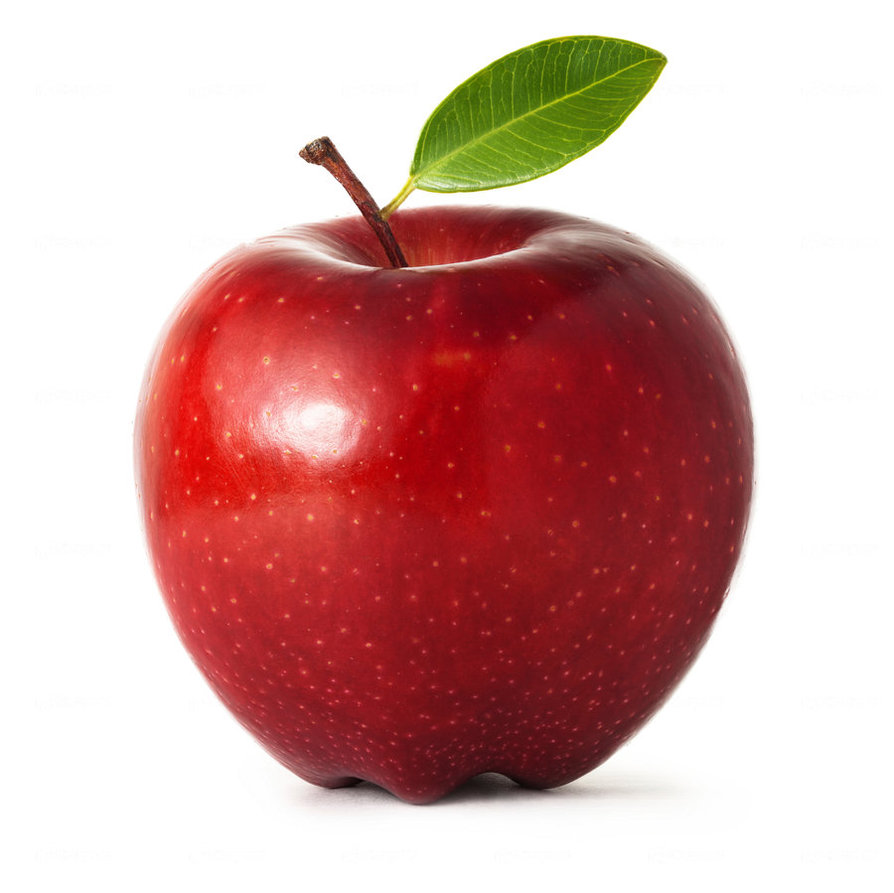
\includegraphics[width=.25\textwidth]{apple.jpg}};
\end{tikzpicture}
}
\savestack{\nnimdbexample}{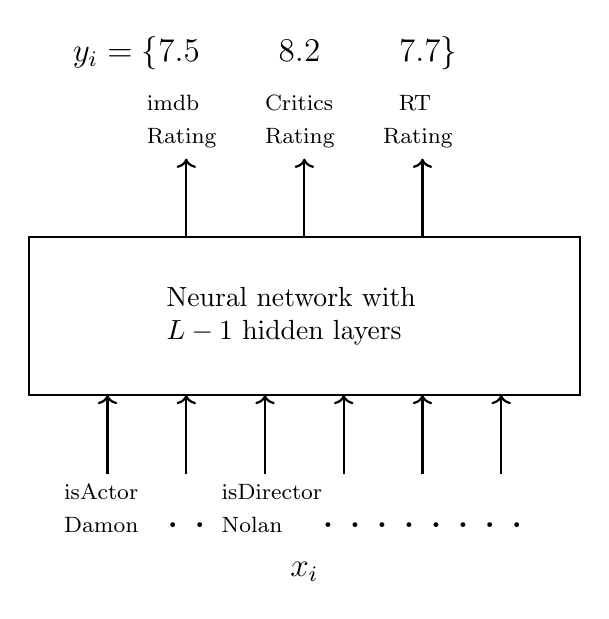
\begin{tikzpicture}[scale=1,transform shape]
	\draw[thick] (0, 0) rectangle (7, 2);
	\draw (3.5,1) node[text width=3.5cm] {Neural network with $L-1$ hidden layers};
	\draw[thick,->] (1,-1) node[below,text width=1.1cm] {\footnotesize isActor Damon} -- (1,0);
	\draw[thick,->] (2,-1) -- (2,0);
	\draw[thick,->] (3,-1) node[below,text width=1.1cm] {\footnotesize isDirector Nolan} -- (3,0);
	\draw[thick,->] (4,-1) -- (4,0);
	\draw[thick,->] (5,-1) -- (5,0);
	\draw[thick,->] (6,-1) -- (6,0);
	\draw[thick,->] (3.5,2) -- (3.5,3) node[above, text width=1cm] {\footnotesize Critics Rating};
	\draw[thick,->] (2,2) -- (2,3) node[above, text width=1cm] {\footnotesize imdb Rating};
	\draw[thick,->] (5,2) -- (5,3) node[above, text width=1cm] {\footnotesize \hspace{0.2cm}RT Rating};
	\draw (2,-1.5) node[below] {\large \textbf{. .}};
	\draw (5,-1.5) node[below] {\large \textbf{. . . . . . . .}};
	\draw (3.5,-2) node[below] {\large $x_i$};
	\draw (3,4) node[above] {\large $y_i = \left\lbrace 7.5 \hspace{1cm} 8.2 \hspace{1cm} 7.7 \right\rbrace$};
\end{tikzpicture}
}
\savestack{\nn}{% \hspace{-0.1in}
\tikzstyle{input_neuron}=[circle,draw=red!50,fill=red!10,thick,minimum size=8mm]
\tikzstyle{hidden_neuron}=[circle,draw=blue!50,fill=cyan!10,thick,minimum size=8mm]
\tikzstyle{output_neuron}=[circle,draw=green!50,fill=green!10,thick,minimum size=8mm]
\tikzstyle{bias_neuron}=[circle,draw=red!50,fill=red!10,thick,minimum size=4mm]
\tikzstyle{bias_hidden_neuron}=[circle,draw=blue!50,fill=cyan!10,thick,minimum size=4mm]
\tikzstyle{input}=[circle,draw=black!50,fill=black!20,thick,minimum size=8mm]
\begin{tikzpicture}
	\node [input_neuron] (neuron01) at (0,0) {$x_1$};
	\node [input_neuron] (neuron02) at (2,0){$x_2$};
	\node [input_neuron] (neuron03) at (4,0) {$x_n$};

	\node [bias_neuron] (neuron04) at (5.2,0.4) {};

	\node [hidden_neuron] (neuron11) at (0,2)  {};
	\node [hidden_neuron] (neuron12) at (2,2)  {};
	\node [hidden_neuron] (neuron13) at (4,2)  {};

	\node [bias_hidden_neuron] (neuron14) at (5.2,2.4) {};

	\begin{scope}
		\path[clip] (0,2) circle (4mm);
		\path[fill=blue!50] (-0.4,2) rectangle (0.4,2.4);
	\end{scope}

	\begin{scope}
		\path[clip] (2,2) circle (4mm);
		\path[fill=blue!50] (1.6,2) rectangle (2.4,2.4);
	\end{scope}

	\begin{scope}
		\path[clip] (4,2) circle (4mm);
		\path[fill=blue!50] (3.6,2) rectangle (4.4,2.4);
	\end{scope}

	\node [hidden_neuron] (neuron21) at (0,4)  {};
	\node [hidden_neuron] (neuron22) at (2,4)  {};
	\node [hidden_neuron] (neuron23) at (4,4)  {};

	\node [bias_hidden_neuron] (neuron24) at (5.2,4.4) {};

	\begin{scope}
		\path[clip] (0,4) circle (4mm);
		\path[fill=blue!50] (-0.4,4) rectangle (0.4,4.4);
	\end{scope}

	\begin{scope}
		\path[clip] (2,4) circle (4mm);
		\path[fill=blue!50] (1.6,4) rectangle (2.4,4.4);
	\end{scope}
	\begin{scope}
		\path[clip] (4,4) circle (4mm);
		\path[fill=blue!50] (3.6,4) rectangle (4.4,4.4);
	\end{scope}

	\node [output_neuron] (neuron31) at (1,6)  {};
	\node [output_neuron] (neuron32) at (3,6)  {};

	\begin{scope}
		\path[clip] (1,6) circle (4mm);
		\path[fill=green!50] (0.6,6) rectangle (1.4,6.4);
	\end{scope}

	\begin{scope}
		\path[clip] (3,6) circle (4mm);
		\path[fill=green!50] (2.6,6) rectangle (3.4,6.4);
	\end{scope}

	\draw[white,->] (neuron01) -- (neuron11) node[black,pos=.5,right]  {$W_{1}$} node[black,pos=0.8,left] {$a_{1}$};

	\draw[white,->] (neuron11) -- (neuron21) node[black,pos=.5,right] {$W_{2}$} node[black,pos=0.8,left] {$a_{2}$} node[black,pos=.2,left] {$h_{1}$};
	\draw[white,->] (neuron21) -- (neuron31) node[black,pos=.5,right] {$W_{3}$} node[black,pos=0.8,left] {$a_{3}$} node[black,pos=.2,left] {$h_{2}$};
	\draw[white,->] (neuron04) -- (neuron13) node[black,pos=0,right,above] {$b_1$};
	\draw[white,->] (neuron14) -- (neuron23) node[black,pos=0,right,above] {$b_2$};
	\draw[white,->] (neuron24) -- (neuron32) node[black,pos=0,right,above] {$b_3$};

	\draw[white,->] (neuron31) -- (1,6.5) node[black,pos=1,above] {$h_L = \hat{y} = f(x)$};

	\draw[black!20,line width=2pt,loosely dotted] (neuron01) -- (neuron02);
	\draw[black!20,line width=2pt,loosely dotted] (neuron02) -- (neuron03);
	\draw[black!20,line width=2pt,loosely dotted] (neuron11) -- (neuron12);
	\draw[black!20,line width=2pt,loosely dotted] (neuron12) -- (neuron13);
	\draw[black!20,line width=2pt,loosely dotted] (neuron21) -- (neuron22);
	\draw[black!20,line width=2pt,loosely dotted] (neuron22) -- (neuron23);
	\draw[black!20,line width=2pt,loosely dotted] (neuron31) -- (neuron32);

	\foreach \from in {neuron01,neuron02,neuron03,neuron04}
	\foreach \to in {neuron11,neuron12,neuron13}
	\draw [black!50,line width=1.5pt,->] (\from) -- (\to);

	\foreach \from in {neuron11,neuron12,neuron13,neuron14}
	\foreach \to in {neuron21,neuron22,neuron23}
	\draw [black!50,line width=1.5pt,->] (\from) -- (\to);

	\foreach \from in {neuron21,neuron22,neuron23,neuron24}
	\foreach \to in {neuron31,neuron32}
	\draw [black!50,line width=1.5pt,->] (\from) -- (\to);
\end{tikzpicture}}


\begin{frame}
  \myheading{Module 4.3: Output Functions and Loss Functions}
\end{frame}

%Slide 11
\begin{frame}
  \begin{block}{We need to answer two questions}
    \begin{itemize}
      \justifying
      \item \alert<2>{How to choose the loss function $\mathscr{L}(\theta)$ ?} \color{black}
      \item How to compute $\nabla \theta$ which is composed of:\\
      $\nabla W_1, \nabla W_2, ..., \nabla W_{L-1} \in \mathbb{R}^{n \times n}, \nabla W_L \in \mathbb{R}^{n \times k}$\\
      $\nabla b_1, \nabla b_2, ..., \nabla b_{L-1} \in \mathbb{R}^n $ and $\nabla b_L \in \mathbb{R}^k$ ?
    \end{itemize}
  \end{block}
\end{frame}

%Slide 12
\begin{frame}
  \begin{columns}
    \column{0.5\textwidth}
    \begin{overlayarea}{\textwidth}{\textheight}
      \vspace{0.3cm}
      \visible<3->{
        \makebox[\textwidth][c]{\usebox{\nnimdbexamplecontent}}
      }
    \end{overlayarea}

    \column{0.5\textwidth}
    \begin{overlayarea}{\textwidth}{\textheight}
      \begin{itemize}[<+->]
      \justifying
        \item The choice of loss function depends on the problem at hand
        \item We will illustrate this with the help of two examples
        \item Consider our movie example again but this time we are interested in predicting ratings
        \item Here $y_i \in \mathbb{R}^3$
        \item The loss function should capture how much $\hat{y}_i$ deviates from $y_i$
        \item If $y_i \in \mathbb{R}^n$ then the squared error loss can capture this deviation
            \vspace{-0.2in}
            \begin{align*}
              \mathscr{L}(\theta) = \frac{1}{N}\sum_{i=1}^{N}\sum_{j=1}^{3}\left(\hat{y}_{ij} - y_{ij}\right)^2
            \end{align*}
      \end{itemize}
    \end{overlayarea}
  \end{columns}
\end{frame}

%Slide 13
\begin{frame}
  \begin{columns}
    \column{0.5\textwidth}
    \begin{overlayarea}{\textwidth}{\textheight}
      \makebox[\textwidth][c]{\usebox{\nncontent}}
    %   \makebox[\textwidth][c]{\usebox{\nnimdbexamplecontent}}
    \end{overlayarea}


    \column{0.5\textwidth}
    \begin{overlayarea}{\textwidth}{\textheight}
      \begin{itemize}[<+->]
      \justifying
        \item A related question: What should the output function `$O$' be if $y_i \in \mathbb{R}$?
        \item More specifically, can it be the logistic function?
        \item No, because it restricts $\hat{y}_i$ to a value between $0$ \& $1$ but we want $\hat{y}_i \in \mathbb{R}$
        \item So, in such cases it makes sense to have `$O$' as linear function
            \begin{align*}
              f(x) & = h_{L} = O(a_{L})             \\
                  &= W_{O}a_{L} + b_{O}
            \end{align*}

        \item $\hat{y}_i = f(x_i)$ is no longer bounded between 0 and 1
      \end{itemize}
    \end{overlayarea}
  \end{columns}
\end{frame}

\begin{frame}[b]
    \visible<1-2>{\tiny Intentionally left blank}
\end{frame}

%Slide 14
\begin{frame}
  \begin{columns}
    \column{0.5\textwidth}
    \begin{overlayarea}{\textwidth}{\textheight}
      \vspace{0.3cm}
      \makebox[\textwidth][c]{\usebox{\nnfruitclassexamplecontent}}
    \end{overlayarea}

    \column{0.5\textwidth}
    \begin{overlayarea}{\textwidth}{\textheight}
      \begin{itemize}[<+->]
      \justifying
        \item Now let us consider another problem for which a different loss function would be appropriate
        \item Suppose we want to classify an image into $1$ of $k$ classes
        \item Here again we could use the squared error loss to capture the deviation
        \item But can you think of a better function?
      \end{itemize}
    \end{overlayarea}
  \end{columns}
\end{frame}

%Slide 15
\begin{frame}
  \begin{columns}
    \column{0.5\textwidth}
    \begin{overlayarea}{\textwidth}{\textheight}
      \only<1-2>{
        \vspace{0.3cm}
        \makebox[\textwidth][c]{\usebox{\nnfruitclassexamplecontent}}
      }
      \only<3->{
        \makebox[\textwidth][c]{\usebox{\nncontent}}
      }
    \end{overlayarea}

    \column{0.5\textwidth}
    \begin{overlayarea}{\textwidth}{\textheight}
      \begin{itemize}
        \justifying
        \item<1-> Notice that $y$ is a probability distribution
        \item<2-> Therefore we should also ensure that $\hat{y}$ is a probability distribution
        \item<3-> What choice of the output activation `$O$' will ensure this ?
            \vspace{-0.1in}
            \begin{align*}
              a_{L}               & = W_{L}h_{L-1} + b_{L}                                            \\
              \visible<4->{\hat{y}_j & = O(a_{L})_j = \frac{e^{a_{L, j}}}{\sum_{i=1}^{k} e^{a_{L,i}}}}
            \end{align*}
            % \vspace{-0.1in}
            \visible<4->{$O(a_{L})_j$ is the $j^{th}$ element of $\hat{y}$ and $a_{L,j}$ is the $j^{th}$ element of the vector $a_{L}$.}
        \item<5-> This function is called the \textit{softmax} function
      \end{itemize}
    \end{overlayarea}
  \end{columns}
\end{frame}

%Slide 16
\begin{frame}
  \begin{columns}
    \column{0.5\textwidth}
    \begin{overlayarea}{\textwidth}{\textheight}
      \vspace{0.3cm}
      \makebox[\textwidth][c]{\usebox{\nnfruitclassexamplecontent}}
    \end{overlayarea}

    \column{0.5\textwidth}
    \begin{overlayarea}{\textwidth}{\textheight}
      \begin{itemize}
        \justifying
        \item<1-> Now that we have ensured that both $y$ \& $\hat{y}$ are probability distributions can you think of a function which captures the difference between them?
        \item<2-> Cross-entropy \begin{equation*}
              \mathscr{L}(\theta) = - \sum_{c=1}^{k} y_c \log \hat{y}_c
            \end{equation*}
        \item<3-> Notice that \begin{align*}
              y_c                 & = 1 \hspace{0.5cm} \text{if $c=\ell$ (the true class label)} \\
                        & = 0 \hspace{0.5cm} \text{otherwise}                          \\
              \therefore~~ &\mathscr{L}(\theta)  = - \log \hat{y}_{\ell}
            \end{align*}
      \end{itemize}
    \end{overlayarea}
  \end{columns}
\end{frame}

%Slide 17
\begin{frame}
  \begin{columns}
    \column{0.35\textwidth}
    \begin{overlayarea}{\textwidth}{\textheight}
      \vspace{0.3cm}
      \makebox[\textwidth][c]{\usebox{\nncontent}}
      % \makebox[\textwidth][c]{\usebox{\nnfruitclassexamplecontent}}
    \end{overlayarea}

    \column{0.65\textwidth}
    \begin{overlayarea}{\textwidth}{\textheight}
      \begin{itemize}[<+->]
      \justifying
        \item So, for classification problem (where you have to choose $1$ of $K$ classes), we use the following objective function
          \begin{align*}
                        \underset{\theta}{\text{minimize}} ~~~~~~\mathscr{L}(\theta) &= -\log \hat{y}_{\ell} \\ %\{- \log \hat{y}_{\ell}\}$ \\ 
              \text{or}~~~~~~\underset{\theta}{\text{maximize}} ~~ -\mathscr{L}(\theta) &=  \log \hat{y}_{\ell}    %\{- \log \hat{y}_{\ell}\}$ \\ 
          \end{align*}
          % \hspace{2cm}
          % \hspace{2cm} 
          %     or $\max \log \hat{y}_{\ell}$
        \item But wait! \\
            Is $\hat{y}_\ell$ a function of $\theta=[W_1,W_2,.,W_L,b_1,b_2,.,b_L]$?
        \item Yes, it is indeed a function of $\theta$
          \begin{center}
            $ \hat y_\ell = [O(W_{3}g(W_{2}g(W_{1}x+b_{1})+b_{2})+b_{3})]_\ell $
          \end{center}
        \item What does $\hat{y}_\ell$ encode? 
        \item It is the probability that $x$ belongs to the $\ell^{th}$ class (bring it as close to $1$).
        \item $\log \hat{y}_\ell$ is called the \textit{log-likelihood} of the data.
      \end{itemize}
    \end{overlayarea}
  \end{columns}
\end{frame}

%Slide 18
\begin{frame}
  \begin{overlayarea}{\textwidth}{\textheight}
    \begin{center}
      \begin{table}[]
        \centering
        \label{my-label}
        \renewcommand{\arraystretch}{2}
        \begin{tabular}{c|c|c|}
          \cline{2-3}
                              & \multicolumn{2}{        c|}{\textbf{Outputs}} \\ \cline{2-3} 
                              & Real Values             & Probabilities     \\ \hline
          \multicolumn{1}{|c|}{Output Activation} & \visible<2->{Linear}       & \alert<7>{\visible<3->{Softmax}}\\ \hline
          \multicolumn{1}{|c|}{Loss Function}     & \visible<4->{Squared Error}& \alert<7>{\visible<5->{Cross Entropy}}   \\ \hline
        \end{tabular}
        \renewcommand{\arraystretch}{1}
      \end{table}
    \end{center}

    \begin{itemize}
      \justifying
      \item<6-> Of course, there could be other loss functions depending on the problem at hand but the two loss functions that we just saw are encountered very often
      \item<7-> For the rest of this lecture we will focus on the case where the output activation is a softmax function and the loss function is cross entropy
    \end{itemize}
  \end{overlayarea}
\end{frame}
  % \savestack{\figuretwo}{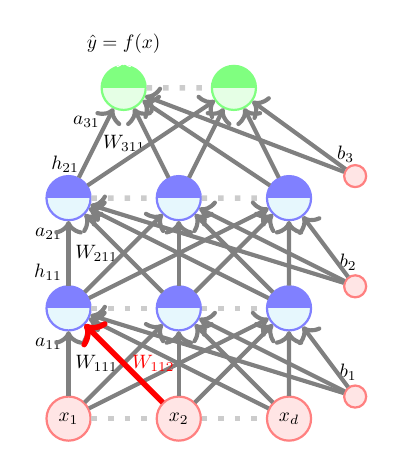
\begin{tikzpicture}[scale=0.7,transform shape]
	\tikzstyle{input_neuron}=[circle,draw=red!50,fill=red!10,thick,minimum size=8mm]
	\tikzstyle{hidden_neuron}=[circle,draw=blue!50,fill=cyan!10,thick,minimum size=8mm]
	\tikzstyle{output_neuron}=[circle,draw=green!50,fill=green!10,thick,minimum size=8mm]
	\tikzstyle{bias_neuron}=[circle,draw=red!50,fill=red!10,thick,minimum size=4mm]

	\tikzstyle{input}=[circle,draw=black!50,fill=black!20,thick,minimum size=8mm]

	\node [input_neuron] (neuron01) at (0,0) {$x_1$};
	\node [input_neuron] (neuron02) at (2,0){$x_2$};
	\node [input_neuron] (neuron03) at (4,0) {$x_d$};

	\node [bias_neuron] (neuron04) at (5.2,0.4) {};


	\node [hidden_neuron] (neuron11) at (0,2)  {};
	\node [hidden_neuron] (neuron12) at (2,2)  {};
	\node [hidden_neuron] (neuron13) at (4,2)  {};

	\node [bias_neuron] (neuron14) at (5.2,2.4) {};

	\begin{scope}
		\path[clip] (0,2) circle (4mm);
		\path[fill=blue!50] (-0.4,2) rectangle (0.4,2.4);
	\end{scope}
	\begin{scope}
		\path[clip] (2,2) circle (4mm);
		\path[fill=blue!50] (1.6,2) rectangle (2.4,2.4);
	\end{scope}
	\begin{scope}
		\path[clip] (4,2) circle (4mm);
		\path[fill=blue!50] (3.6,2) rectangle (4.4,2.4);
	\end{scope}


	\node [hidden_neuron] (neuron21) at (0,4)  {};
	\node [hidden_neuron] (neuron22) at (2,4)  {};
	\node [hidden_neuron] (neuron23) at (4,4)  {};

	\node [bias_neuron] (neuron24) at (5.2,4.4) {};


	\begin{scope}
		\path[clip] (0,4) circle (4mm);
		\path[fill=blue!50] (-0.4,4) rectangle (0.4,4.4);
	\end{scope}
	\begin{scope}
		\path[clip] (2,4) circle (4mm);
		\path[fill=blue!50] (1.6,4) rectangle (2.4,4.4);
	\end{scope}
	\begin{scope}
		\path[clip] (4,4) circle (4mm);
		\path[fill=blue!50] (3.6,4) rectangle (4.4,4.4);
	\end{scope}



	\node [output_neuron] (neuron31) at (1,6)  {};
	\node [output_neuron] (neuron32) at (3,6)  {};



	\begin{scope}
		\path[clip] (1,6) circle (4mm);
		\path[fill=green!50] (0.6,6) rectangle (1.4,6.4);
	\end{scope}
	\begin{scope}
		\path[clip] (3,6) circle (4mm);
		\path[fill=green!50] (2.6,6) rectangle (3.4,6.4);
	\end{scope}

	\draw[white,->] (neuron01) -- (neuron11) node[black,pos=.5,right]  {$W_{111}$} node[black,pos=0.8,left] {$a_{11}$};

	\draw[white,->] (neuron11) -- (neuron21) node[black,pos=.5,right] {$W_{211}$} node[black,pos=0.8,left] {$a_{21}$} node[black,pos=.2,left] {$h_{11}$};
	\draw[white,->] (neuron21) -- (neuron31) node[black,pos=.5,right] {$W_{311}$} node[black,pos=0.8,left] {$a_{31}$} node[black,pos=.2,left] {$h_{21}$};

	\draw[white,->] (neuron04) -- (neuron13) node[black,pos=0,right,above] {$b_1$};

	\draw[white,->] (neuron14) -- (neuron23) node[black,pos=0,right,above] {$b_2$};

	\draw[white,->] (neuron24) -- (neuron32) node[black,pos=0,right,above] {$b_3$};



	\draw[white,->] (neuron31) -- (1,6.5) node[black,pos=1,above] {$\hat{y} = f(x)$};
	%\draw[white,->] (neuron31) -- (3,6.5) node[black,pos=1,above] {$f(x)$};
	%node[pos=1.3,above,right] {$\mathscr{L}(\theta)$};

	\draw[black!20,line width=2pt,loosely dotted] (neuron01) -- (neuron02);
	\draw[black!20,line width=2pt,loosely dotted] (neuron02) -- (neuron03);
	\draw[black!20,line width=2pt,loosely dotted] (neuron11) -- (neuron12);
	\draw[black!20,line width=2pt,loosely dotted] (neuron12) -- (neuron13);
	\draw[black!20,line width=2pt,loosely dotted] (neuron21) -- (neuron22);
	\draw[black!20,line width=2pt,loosely dotted] (neuron22) -- (neuron23);
	\draw[black!20,line width=2pt,loosely dotted] (neuron31) -- (neuron32);


	\foreach \from in {neuron01,neuron02,neuron03,neuron04}
	\foreach \to in {neuron11,neuron12,neuron13}
	\draw [black!50,line width=1.5pt,->] (\from) -- (\to);

	\foreach \from in {neuron11,neuron12,neuron13,neuron14}
	\foreach \to in {neuron21,neuron22,neuron23}
	\draw [black!50,line width=1.5pt,->] (\from) -- (\to);

	\foreach \from in {neuron21,neuron22,neuron23,neuron24}
	\foreach \to in {neuron31,neuron32}
	\draw [black!50,line width=1.5pt,->] (\from) -- (\to);

	\draw [red,line width=2pt,->] (neuron02) -- (neuron11) node[pos=0.5,right] {$W_{112}$};

\end{tikzpicture}}
\savestack{\figurethree}{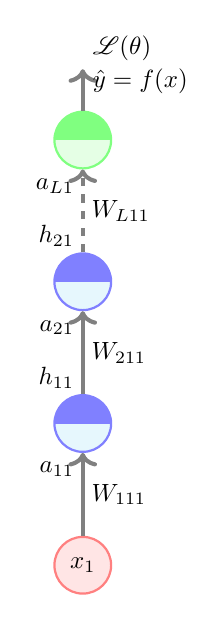
\begin{tikzpicture}[scale=0.9,transform shape]
	\tikzstyle{input_neuron}=[circle,draw=red!50,fill=red!10,thick,minimum size=8mm]
	\tikzstyle{hidden_neuron}=[circle,draw=blue!50,fill=cyan!10,thick,minimum size=8mm]
	\tikzstyle{output_neuron}=[circle,draw=green!50,fill=green!10,thick,minimum size=8mm]


	\node [input_neuron] (neuron01) at (0,0) {$x_1$};
	\node [hidden_neuron] (neuron11) at (0,2)  {};

	\begin{scope}
		\path[clip] (0,2) circle (4mm);
		\path[fill=blue!50] (-0.4,2) rectangle (0.4,2.4);
	\end{scope}


	\node [hidden_neuron] (neuron21) at (0,4)  {};


	\begin{scope}
		\path[clip] (0,4) circle (4mm);
		\path[fill=blue!50] (-0.4,4) rectangle (0.4,4.4);
	\end{scope}

	\node [output_neuron] (neuron31) at (0,6)  {};



	\begin{scope}
		\path[clip] (0,6) circle (4mm);
		\path[fill=green!50] (-0.4,6) rectangle (0.4,6.4);
	\end{scope}

	\draw[white,->] (neuron01) -- (neuron11) node[black,pos=.5,right]  {$W_{111}$} node[black,pos=0.8,left] {$a_{11}$};

	\draw[white,->] (neuron11) -- (neuron21) node[black,pos=.5,right] {$W_{211}$} node[black,pos=0.8,left] {$a_{21}$} node[black,pos=.2,left] {$h_{11}$};
	\draw[white,->] (neuron21) -- (neuron31) node[black,pos=.5,right] {$W_{L11}$} node[black,pos=0.8,left] {$a_{L1}$} node[black,pos=.2,left] {$h_{21}$};


	\draw[black!50,line width=1.5pt,->] (neuron31) -- (0,7) node[black,pos=0.7,right] {$\hat{y} = f(x)$} node[black,pos=1.5,above,right] {$\mathscr{L}(\theta)$};
	%\draw[white,->] (neuron31) -- (3,6.5) node[black,pos=1,above] {$f(x)$};
	%node[pos=1.3,above,right] {$\mathscr{L}(\theta)$};


	\foreach \from in {neuron01}
	\foreach \to in {neuron11}
	\draw [black!50,line width=1.5pt,->] (\from) -- (\to);

	\foreach \from in {neuron11}
	\foreach \to in {neuron21}
	\draw [black!50,line width=1.5pt,->] (\from) -- (\to);

	\foreach \from in {neuron21}
	\foreach \to in {neuron31}
	\draw [black!50,line width=1.5pt,dashed,->] (\from) -- (\to);


\end{tikzpicture}}

\begin{frame}
  \myheading{Module 4.4: Backpropagation (Intuition)}
\end{frame}

%Slide 19
\begin{frame}
  \begin{block}{We need to answer two questions}
    \begin{itemize}
      \justifying
      \item How to choose the loss function $\mathscr{L}(\theta)$ ?
      \item \alert<2->{How to compute $\nabla \theta$ which is composed of:\\
      $\nabla W_1, \nabla W_2, ..., \nabla W_{L-1} \in \mathbb{R}^{n \times n}, \nabla W_{L} \in \mathbb{R}^{n \times k}$\\
      $\nabla b_1, \nabla b_2, ..., \nabla b_{L-1} \in \mathbb{R}^n $ and $\nabla b_{L} \in \mathbb{R}^k$ ?}
    \end{itemize}
  \end{block}
\end{frame}

%Slide 20
\begin{frame}
  \begin{columns}
    \column{0.33\textwidth}
    \begin{overlayarea}{\textwidth}{\textheight}
      \begin{itemize}
        \justifying
        \item<1-> Let us focus on this one weight ($W_{112}$).
        \item<2-> To learn this weight using SGD we need a formula for $\frac{\partial \mathscr{L}(\theta)}{ \partial W_{112}}$.
        \item<3-> We will see how to calculate this.
      \end{itemize}
    \end{overlayarea}

    \column{0.33\textwidth}

    \begin{overlayarea}{\textwidth}{\textheight}
      \makebox[\textwidth][c]{\usebox{\figuretwocontent}}
    \end{overlayarea}

    \column{0.33\textwidth}
    \begin{overlayarea}{\textwidth}{\textheight}
      \begin{algorithm}[H]
        \SetAlgoLined
        $t \leftarrow 0$\;
        $max\_iterations\leftarrow 1000$\;
        $Initialize \quad \theta_0$\;
        \color{black}
        \While{$t\texttt{++} < max\_iterations$}{
          $\theta_{t+1} \leftarrow \theta_{t} - \eta \nabla \theta_{t}$\;
        }
        \caption{gradient descent()}
      \end{algorithm}
    \end{overlayarea}
  \end{columns}
\end{frame}

%Slide 21
\begin{frame}
  \begin{columns}
    \column{0.53\textwidth}
    \begin{overlayarea}{\textwidth}{\textheight}
      \begin{itemize}[<+->]
      \justifying
        \item First let us take the simple case when we have a deep but thin network.
        \item In this case it is easy to find the derivative by chain rule.
      \end{itemize}
      \begin{align*}
        \visible<3->{
        \frac{\partial \mathscr{L}(\theta)}{\partial W_{111}} & = \color<6>{red}{\color<4->{red}{\color<5>{red}{\frac{\partial \mathscr{L}(\theta)}{\partial \hat{y}} \frac{\partial \hat{y}}{\partial a_{L11}}} \color<6>{red}{\frac{\partial a_{L11}}{\partial h_{21}}} \color<5>{red}{\frac{\partial h_{21}}{\partial a_{21}} \frac{\partial a_{21}}{\partial h_{11}}} \color<4->{blue}{\frac{\partial h_{11}}{\partial a_{11}} \frac{\partial a_{11}}{\partial W_{111}}}}}
        }\\
        \visible<4->{
        \frac{\partial \mathscr{L}(\theta)}{\partial W_{111}} & = \color<4->{red}{\frac{\partial \mathscr{L}(\theta)}{\partial h_{11}}}
          \color<4->{blue}{\frac{\partial h_{11}}{\partial W_{111}}} ~~~~ \color<4->{black}\text{(just compressing the chain rule)}
        } \\
        \visible<5->{
        \frac{\partial \mathscr{L}(\theta)}{\partial W_{211}} & = \frac{\partial \mathscr{L}(\theta)}{\partial h_{21}}
          \frac{\partial h_{21}}{\partial W_{211}}
        } \\
        \visible<6->{
        \frac{\partial \mathscr{L}(\theta)}{\partial W_{L11}} & = \frac{\partial \mathscr{L}(\theta)}{\partial a_{L1}}
          \frac{\partial a_{L1}}{\partial W_{L11}}
        }
      \end{align*}
    \end{overlayarea}

    \column{0.47\textwidth}
    \begin{overlayarea}{\textwidth}{\textheight}
      % \only<1-6>{
          \makebox[\textwidth][c]{\usebox{\figurethreecontent}}
      % }
      % \only<7->{
      %   \begin{itemize}
      \justifying
      %     \item <7->  Observe that if we come up with a generic formula:
      %         \begin{align*}
      %           \visible<7->{ & \frac{\partial \mathscr{L}(\theta)}{\partial h_{ij}} \text{\hspace{1em}(gradient w.r.t. hidden units)}}     \\
      %           \visible<8->{ & \frac{\partial \mathscr{L}(\theta)}{\partial a_{L,j}} \text{\hspace{0.1em} (gradient w.r.t. output units)}} \\
      %           \visible<9->{ & \frac{\partial h_{ij}}{\partial W_{ij}} \text{\hspace{1em} (gradient w.r.t. weights)}}
      %         \end{align*}
      %         \visible<10->{\noindent then we can compute all the required gradients}
      %     \item <11->  This is called the backpropagation algorithm because the loss gets propagated all the way back to the weights.
      %   \end{itemize}
      % }
    \end{overlayarea}
  \end{columns}
\end{frame}

%Slide 22
\begin{frame}
  Let us see an intuitive explanation of backpropagation before we get into the mathematical details
\end{frame}

%Slide 23
\begin{frame}
  \begin{columns}
    \column{0.6\textwidth}
    \begin{overlayarea}{\textwidth}{\textheight}
      \visible{
        \small{
          \begin{itemize}
            \justifying

            \justifying
            \item<1-> We get a certain loss at the output and we try to figure out who is responsible for this loss

            \item<2-> So, we talk to the output layer and say ``Hey! You are not producing the desired output, better take responsibility".

            \item<3-> The output layer says ``Well, I take responsibility for my part but please understand that I am only as the good as the hidden layer and weights below me". After all $\dots$
                $$ f(x) = \hat{y} = O(W_{L}h_{L-1}+b_{L}) $$

          \end{itemize}
        }
      }
    \end{overlayarea}

    \column{0.4\textwidth}
    \begin{overlayarea}{\textwidth}{\textheight}
      \hspace{-0.1in}
\tikzstyle{input_neuron}=[circle,draw=red!50,fill=red!10,thick,minimum size=5mm]
\tikzstyle{hidden_neuron}=[circle,draw=blue!50,fill=cyan!10,thick,minimum size=6mm]
\tikzstyle{output_neuron}=[circle,draw=green!50,fill=green!10,thick,minimum size=6mm]
\tikzstyle{bias_neuron}=[circle,draw=red!50,fill=red!10,thick,minimum size=2mm]
\tikzstyle{bias_hidden_neuron}=[circle,draw=blue!50,fill=cyan!10,thick,minimum size=2mm]
\tikzstyle{bias_hidden_neuron_hi}=[circle,draw=orange,fill=cyan!10,thick,minimum size=2mm]
\tikzstyle{input}=[circle,draw=black!50,fill=black!20,thick,minimum size=6mm]

\begin{tikzpicture}
	\node [input_neuron] (neuron01) at (0,0) {$x_1$};
	\node [input_neuron] (neuron02) at (2,0){$x_2$};
	\node [input_neuron] (neuron03) at (4,0) {$x_n$};

	\node [bias_neuron] (neuron04) at (5.2,0.4) {};

	\node [hidden_neuron] (neuron11) at (0,1.7)  {};
	\node [hidden_neuron] (neuron12) at (2,1.7)  {};
	\node [hidden_neuron] (neuron13) at (4,1.7)  {};

	\node [bias_hidden_neuron] (neuron14) at (5.2,2.1) {};

	\begin{scope}
		\path[clip] (0,1.7) circle (3mm);
		\path[fill=blue!50] (-0.4,1.7) rectangle (0.3,2);
	\end{scope}
	\begin{scope}
		\path[clip] (2,1.7) circle (3mm);
		\path[fill=blue!50] (1.6,1.7) rectangle (2.3,2);
	\end{scope}
	\begin{scope}
		\path[clip] (4,1.7) circle (3mm);
		\path[fill=blue!50] (3.6,1.7) rectangle (4.3,2);
	\end{scope}


	\node [hidden_neuron] (neuron21) at (0,3.4)  {};
	\node [hidden_neuron] (neuron22) at (2,3.4)  {};
	\node [hidden_neuron] (neuron23) at (4,3.4)  {};

	\onslide<1-2>{\node [bias_hidden_neuron] (neuron24) at (5.2,3.7) {};}
	\onslide<3> {\node [bias_hidden_neuron_hi] (neuron24) at (5.2,3.7) {};}

	\begin{scope}
		\path[clip] (0,3.4) circle (3mm);
		\path[fill=blue!50] (-0.4,3.4) rectangle (0.4,3.7);
	\end{scope}
	\begin{scope}
		\path[clip] (2,3.4) circle (3mm);
		\path[fill=blue!50] (1.6,3.4) rectangle (2.4,3.7);
	\end{scope}
	\begin{scope}
		\path[clip] (4,3.4) circle (3mm);
		\path[fill=blue!50] (3.6,3.4) rectangle (4.4,3.7);
	\end{scope}


	\node [output_neuron] (neuron31) at (1,5.1)  {};
	\node [output_neuron] (neuron32) at (3,5.1)  {};
	\onslide<1->{\draw [fill=gray] (1, 7) rectangle (3, 6.5) node[pos=0.5] {$-\log\hat{y}_\ell$};}
	%\onslide<2->{\draw [fill=yellow!50] (1, 7) rectangle (3, 6.5) node[pos=0.5] {$-\log\hat{y}_\ell$};}
	\onslide<1>{\draw [black!50,line width=1.5pt,  ->] (1, 5.4) -- (1.8, 6.5);}
	\onslide<1>{\draw [black!50, line width=1.5pt, ->]  (3, 5.4) -- (2.2, 6.5);}
	\onslide<2->{\draw [yellow,line width=1.5pt,  ->] (1.8, 6.5) -- (1, 5.4);}
	\onslide<2->{\draw [yellow, line width=1.5pt, ->]  (2.2, 6.5) -- (3, 5.4);}
	\onslide<2>{\draw [orange, line width = 3] (1.3,5.1) arc (0:180:3mm) {};}
	\onslide<2>{\draw [orange, line width = 3] (3.3,5.1) arc (0:180:3mm) {};}
	\onslide<3>{\draw [yellow, line width = 3] (1.3,5.1) arc (0:180:3mm) {};}
	\onslide<3>{\draw [yellow, line width = 3] (3.3,5.1) arc (0:180:3mm) {};}
	\onslide<3>{\draw[yellow, line width = 2] (0.7, 5.1) arc (180:360:3mm){};}
	\onslide<3>{\draw[yellow, line width = 2] (2.7, 5.1) arc (180:360:3mm){};}
	\onslide<3>{\draw[orange, line width = 2] (0.3, 3.4) arc (0:180:3mm){};}
	\onslide<3>{\draw[orange, line width = 2] (2.3, 3.4) arc (0:180:3mm){};}
	\onslide<3>{\draw[orange, line width = 2] (4.3, 3.4) arc (0:180:3mm){};}


	\begin{scope}
		\path[clip] (1,5.1) circle (3mm);
		\path[fill=green!50] (0.6,5.1) rectangle (1.3,5.4);
	\end{scope}
	\begin{scope}
		\path[clip] (3,5.1) circle (3mm);
		\path[fill=green!50] (2.6,5.1) rectangle (3.3,5.4);
	\end{scope}

	\draw[white,->] (neuron01) -- (neuron11) node[black,pos=.5,right]  {$W_{1}$} node[black,pos=0.8,left] {$a_{1}$};

	\draw[white,->] (neuron11) -- (neuron21) node[black,pos=.5,right] {$W_{2}$} node[black,pos=0.8,left] {$a_{2}$} node[black,pos=.2,left] {$h_{1}$};
	\draw[white,->] (neuron21) -- (neuron31) node[black,pos=.5,right] {$W_{3}$} node[black,pos=0.8,left] {$a_{3}$} node[black,pos=.2,left] {$h_{2}$};

	\draw[white,->] (neuron04) -- (neuron13) node[black,pos=0,right,above] {$b_1$};

	\draw[white,->] (neuron14) -- (neuron23) node[black,pos=0,right,above] {$b_2$};

	\draw[white,->] (neuron24) -- (neuron32) node[black,pos=0,right,above] {$b_3$};

	\draw[black!20,line width=2pt,loosely dotted] (neuron01) -- (neuron02);
	\draw[black!20,line width=2pt,loosely dotted] (neuron02) -- (neuron03);
	\draw[black!20,line width=2pt,loosely dotted] (neuron11) -- (neuron12);
	\draw[black!20,line width=2pt,loosely dotted] (neuron12) -- (neuron13);
	\draw[black!20,line width=2pt,loosely dotted] (neuron21) -- (neuron22);
	\draw[black!20,line width=2pt,loosely dotted] (neuron22) -- (neuron23);
	\draw[black!20,line width=2pt,loosely dotted] (neuron31) -- (neuron32);


	\foreach \from in {neuron01,neuron02,neuron03,neuron04}
	\foreach \to in {neuron11,neuron12,neuron13}
	\draw [black!50,line width=1.5pt,->] (\from) -- (\to);

	\foreach \from in {neuron11,neuron12,neuron13,neuron14}
	\foreach \to in {neuron21,neuron22,neuron23}
	\draw [black!50,line width=1.5pt,->] (\from) -- (\to);

	\foreach \from in {neuron21,neuron24,neuron23, neuron22}
	\foreach \to in {neuron31,neuron32}
		{\onslide<1-2>{\draw [black!50,line width=1.5pt,->] (\from) -- (\to);}}

	\foreach \from in {neuron21,neuron24,neuron23, neuron22}
	\foreach \to in {neuron31,neuron32}
		{\onslide<3>{\draw [yellow,line width=1.5pt,->] (\to) -- (\from);}}


\end{tikzpicture}

    \end{overlayarea}
  \end{columns}
\end{frame}


%Slide 24
\begin{frame}
  \begin{columns}
    \column{0.6\textwidth}
    \begin{overlayarea}{\textwidth}{\textheight}
      \footnotesize{
        \begin{itemize}
          \justifying
          \item So, we talk to $W_{L},b_{L}$ and $h_{L}$ and ask them ``What is wrong with you?"
          \item<2-> $W_{L}$ and $b_{L}$ take full responsibility but $h_{L}$ says ``Well, please understand that I am only as good as the pre-activation layer"
          \item<3-> The pre-activation layer in turn says that I am only as good as the hidden layer and weights below me.
          \item<4-> We continue in this manner and realize that the responsibility lies with all the weights and biases (i.e. all the parameters of the model)
          \item<5-> But instead of talking to them directly, it is easier to talk to them through the hidden layers and output layers (and this is exactly what the chain rule allows us to do)
              \visible<6->{
                \begin{align*}
                  \underbrace{\frac{\partial \mathscr{L}(\theta)}{\partial W_{111}}}_
                  {\substack{\text{Talk to the}\\ \text{weight directly}}}
                  =
                  \underbrace{\frac{\partial \mathscr{L}(\theta)}{\partial \hat{y}} \frac{\partial \hat{y}}{\partial a_{3}}}_
                  {\substack{\text{Talk to the} \\ \text{output layer}}}
                  \underbrace{\frac{\partial a_{3}}{\partial h_{2}} \frac{\partial h_{2}}{\partial a_{2}}}_
                  {\substack{\text{Talk to the} \\ \text{previous hidden} \\ \text{layer}}}
                  \underbrace{\frac{\partial a_{2}}{\partial h_{1}} \frac{\partial h_{1}}{\partial a_{1}}}_
                  {\substack{\text{Talk to the} \\ \text{previous} \\ \text{hidden layer}}}
                  \underbrace{\frac{\partial a_{1}}{\partial W_{111}}}_
                  {\substack{\text{and now} \\ \text{talk to} \\ \text{the} \\ \text{weights}}}
                \end{align*}
              }
        \end{itemize}
      }
    \end{overlayarea}

    \column{0.4\textwidth}
    \begin{overlayarea}{\textwidth}{\textheight}
      \hspace{-0.1in}
\tikzstyle{input_neuron}=[circle,draw=red!50,fill=red!10,thick,minimum size=5mm]
\tikzstyle{hidden_neuron}=[circle,draw=blue!50,fill=cyan!10,thick,minimum size=6mm]
\tikzstyle{output_neuron}=[circle,draw=green!50,fill=green!10,thick,minimum size=6mm]
\tikzstyle{bias_neuron}=[circle,draw=red!50,fill=red!10,thick,minimum size=2mm]
\tikzstyle{bias_hidden_neuron}=[circle,draw=blue!50,fill=cyan!10,thick,minimum size=2mm]
\tikzstyle{bias_hidden_neuron_hi}=[circle,draw=orange,fill=cyan!10,thick,minimum size=2mm]
\tikzstyle{bias_hidden_neuron_hi_old}=[circle,draw=yellow,fill=cyan!10,thick,minimum size=2mm]
\tikzstyle{input}=[circle,draw=black!50,fill=black!20,thick,minimum size=6mm]
\begin{tikzpicture}
	\node [input_neuron] (neuron01) at (0,0) {$x_1$};
	\node [input_neuron] (neuron02) at (2,0){$x_2$};
	\node [input_neuron] (neuron03) at (4,0) {$x_n$};

	\node [bias_neuron] (neuron04) at (5.2,0.4) {};

	\node [hidden_neuron] (neuron11) at (0,1.7)  {};
	\node [hidden_neuron] (neuron12) at (2,1.7)  {};
	\node [hidden_neuron] (neuron13) at (4,1.7)  {};

	\node [bias_hidden_neuron] (neuron14) at (5.2,2.1) {};

	\begin{scope}
		\path[clip] (0,1.7) circle (3mm);
		\path[fill=blue!50] (-0.4,1.7) rectangle (0.3,2);
	\end{scope}
	\begin{scope}
		\path[clip] (2,1.7) circle (3mm);
		\path[fill=blue!50] (1.6,1.7) rectangle (2.3,2);
	\end{scope}
	\begin{scope}
		\path[clip] (4,1.7) circle (3mm);
		\path[fill=blue!50] (3.6,1.7) rectangle (4.3,2);
	\end{scope}


	\node [hidden_neuron] (neuron21) at (0,3.4)  {};
	\node [hidden_neuron] (neuron22) at (2,3.4)  {};
	\node [hidden_neuron] (neuron23) at (4,3.4)  {};


	\onslide<1> {\node [bias_hidden_neuron_hi] (neuron24) at (5.2,3.7) {};}
	\onslide<2-> {\node [bias_hidden_neuron_hi_old] (neuron24) at (5.2,3.7) {};}
	\begin{scope}
		\path[clip] (0,3.4) circle (3mm);
		\path[fill=blue!50] (-0.4,3.4) rectangle (0.4,3.7);
	\end{scope}
	\begin{scope}
		\path[clip] (2,3.4) circle (3mm);
		\path[fill=blue!50] (1.6,3.4) rectangle (2.4,3.7);
	\end{scope}
	\begin{scope}
		\path[clip] (4,3.4) circle (3mm);
		\path[fill=blue!50] (3.6,3.4) rectangle (4.4,3.7);
	\end{scope}


	\node [output_neuron] (neuron31) at (1,5.1)  {};
	\node [output_neuron] (neuron32) at (3,5.1)  {};
	\onslide<1->{\draw [fill=gray] (1, 7) rectangle (3, 6.5) node[pos=0.5] {$-\log\hat{y}_\ell$};}

	\onslide<1->{\draw [yellow,line width=1.5pt,  ->] (1.8, 6.5) -- (1, 5.4);}
	\onslide<1->{\draw [yellow, line width=1.5pt, ->]  (2.2, 6.5) -- (3, 5.4);}

	\onslide<1->{\draw [yellow, line width = 3] (1.3,5.1) arc (0:180:3mm) {};}
	\onslide<1->{\draw [yellow, line width = 3] (3.3,5.1) arc (0:180:3mm) {};}
	\onslide<1->{\draw[yellow, line width = 2] (0.7, 5.1) arc (180:360:3mm){};}
	\onslide<1->{\draw[yellow, line width = 2] (2.7, 5.1) arc (180:360:3mm){};}
	\onslide<1->{\draw[orange, line width = 2] (0.3, 3.4) arc (0:180:3mm){};}
	\onslide<1->{\draw[orange, line width = 2] (2.3, 3.4) arc (0:180:3mm){};}
	\onslide<1->{\draw[orange, line width = 2] (4.3, 3.4) arc (0:180:3mm){};}

	\onslide<2->{\draw[yellow, line width = 2] (0.3, 3.4) arc (0:180:3mm){};}
	\onslide<2->{\draw[yellow, line width = 2] (2.3, 3.4) arc (0:180:3mm){};}
	\onslide<2->{\draw[yellow, line width = 2] (4.3, 3.4) arc (0:180:3mm){};}
	\onslide<2>{\draw[orange, line width = 2] (-0.3, 3.4) arc (180:360:3mm){};}
	\onslide<2>{\draw[orange, line width = 2] (1.7, 3.4) arc (180:360:3mm){};}
	\onslide<2>{\draw[orange, line width = 2] (3.7, 3.4) arc (180:360:3mm){};}
	\onslide<3->{\draw[yellow, line width = 2] (-0.3, 3.4) arc (180:360:3mm){};}
	\onslide<3->{\draw[yellow, line width = 2] (1.7, 3.4) arc (180:360:3mm){};}
	\onslide<3->{\draw[yellow, line width = 2] (3.7, 3.4) arc (180:360:3mm){};}

	\onslide<3>{\draw[orange, line width = 2] (0.3, 1.7) arc (0:180:3mm){};}
	\onslide<3>{\draw[orange, line width = 2] (2.3, 1.7) arc (0:180:3mm){};}
	\onslide<3>{\draw[orange, line width = 2] (4.3, 1.7) arc (0:180:3mm){};}
	\onslide<3> {\node [bias_hidden_neuron_hi] (neuron14) at (5.2,2.1) {};}

	\onslide<4->{\draw[yellow, line width = 2] (0.3, 1.7) arc (0:180:3mm){};}
	\onslide<4->{\draw[yellow, line width = 2] (2.3, 1.7) arc (0:180:3mm){};}
	\onslide<4->{\draw[yellow, line width = 2] (4.3, 1.7) arc (0:180:3mm){};}
	\onslide<4-> {\node [bias_hidden_neuron_hi_old] (neuron14) at (5.2,2.1) {};}

	\onslide<4>{\draw[orange, line width = 2] (-0.3, 1.7) arc (180:360:3mm){};}
	\onslide<4>{\draw[orange, line width = 2] (1.7, 1.7) arc (180:360:3mm){};}
	\onslide<4>{\draw[orange, line width = 2] (3.7, 1.7) arc (180:360:3mm){};}

	\onslide<5->{\draw[orange, line width = 2] (-0.3, 1.7) arc (180:360:3mm){};}
	\onslide<5->{\draw[orange, line width = 2] (1.7, 1.7) arc (180:360:3mm){};}
	\onslide<5->{\draw[orange, line width = 2] (3.7, 1.7) arc (180:360:3mm){};}

	\begin{scope}
		\path[clip] (1,5.1) circle (3mm);
		\path[fill=green!50] (0.6,5.1) rectangle (1.3,5.4);
	\end{scope}
	\begin{scope}
		\path[clip] (3,5.1) circle (3mm);
		\path[fill=green!50] (2.6,5.1) rectangle (3.3,5.4);
	\end{scope}

	\draw[white,->] (neuron01) -- (neuron11) node[black,pos=.5,right]  {$W_{1}$} node[black,pos=0.8,left] {$a_{1}$};

	\draw[white,->] (neuron11) -- (neuron21) node[black,pos=.5,right] {$W_{2}$} node[black,pos=0.8,left] {$a_{2}$} node[black,pos=.2,left] {$h_{1}$};
	\draw[white,->] (neuron21) -- (neuron31) node[black,pos=.5,right] {$W_{3}$} node[black,pos=0.8,left] {$a_{3}$} node[black,pos=.2,left] {$h_{2}$};

	\draw[white,->] (neuron04) -- (neuron13) node[black,pos=0,right,above] {$b_1$};

	\draw[white,->] (neuron14) -- (neuron23) node[black,pos=0,right,above] {$b_2$};

	\draw[white,->] (neuron24) -- (neuron32) node[black,pos=0,right,above] {$b_3$};


	%\draw[white,->] (neuron31) -- (2.4.9) node[black,pos=1,above] {y };
	%\draw[white,->] (neuron31) -- (3,6.5) node[black,pos=1,above] {$f(x)$};
	%node[pos=1.3,above,right] {$\mathscr{L}(\theta)$};

	\draw[black!20,line width=2pt,loosely dotted] (neuron01) -- (neuron02);
	\draw[black!20,line width=2pt,loosely dotted] (neuron02) -- (neuron03);
	\draw[black!20,line width=2pt,loosely dotted] (neuron11) -- (neuron12);
	\draw[black!20,line width=2pt,loosely dotted] (neuron12) -- (neuron13);
	\draw[black!20,line width=2pt,loosely dotted] (neuron21) -- (neuron22);
	\draw[black!20,line width=2pt,loosely dotted] (neuron22) -- (neuron23);
	\draw[black!20,line width=2pt,loosely dotted] (neuron31) -- (neuron32);


	\foreach \from in {neuron01,neuron02,neuron03,neuron04}
	\foreach \to in {neuron11,neuron12,neuron13}
		{\onslide<1-4>{\draw [black!50,line width=1.5pt,->] (\from) -- (\to);}}


	\foreach \from in {neuron01,neuron02,neuron03,neuron04}
	\foreach \to in {neuron11,neuron12,neuron13}
		{\onslide<5->{\draw [yellow,line width=1.5pt,->] (\to) -- (\from);}}

	\foreach \from in {neuron11,neuron12,neuron13,neuron14}
	\foreach \to in {neuron21,neuron22,neuron23}
		{\onslide<1-2>{\draw [black!50,line width=1.5pt,->] (\from) -- (\to);}}

	\foreach \from in {neuron11,neuron12,neuron13,neuron14}
	\foreach \to in {neuron21,neuron22,neuron23}
		{\onslide<3->{\draw [yellow, line width=1.5pt,->] (\to) -- (\from);}}


	%\foreach \from in {neuron21,neuron24,neuron23, neuron22}
	%	\foreach \to in {neuron31,neuron32}
	%		{\onslide<1-2>{\draw [black!50,line width=1.5pt,->] (\from) -- (\to);}}

	\foreach \from in {neuron21,neuron24,neuron23, neuron22}
	\foreach \to in {neuron31,neuron32}
		{\onslide<1->{\draw [yellow,line width=1.5pt,->] (\to) -- (\from);}}


\end{tikzpicture}

    \end{overlayarea}
  \end{columns}
\end{frame}

%Slide 25
\begin{frame}
  \begin{overlayarea}{\textwidth}{\textheight}
    \visible<2->{\textbf{Quantities of interest (roadmap for the remaining part):}}
    \begin{itemize}
      \justifying
      \item<3-> Gradient w.r.t. output units
      \item<4-> Gradient w.r.t. hidden units
      \item<5-> Gradient w.r.t. weights and biases
    \end{itemize}

    \begin{align*}
      \underbrace{\frac{\partial \mathscr{L}(\theta)}{\partial W_{111}}}_
      {\substack{\text{Talk to the}\\ \text{weight directly}}}
      =
      \underbrace{\frac{\partial \mathscr{L}(\theta)}{\partial \hat{y}} \frac{\partial \hat{y}}{\partial a_{3}}}_
        {\substack{\text{Talk to the} \\ \text{output layer}}}
      \underbrace{\frac{\partial a_{3}}{\partial h_{2}} \frac{\partial h_{2}}{\partial a_{2}}}_
      {\substack{\text{Talk to the} \\ \text{previous hidden} \\ \text{layer}}}
      \underbrace{\frac{\partial a_{2}}{\partial h_{1}} \frac{\partial h_{1}}{\partial a_{1}}}_
      {\substack{\text{Talk to the} \\ \text{previous} \\ \text{hidden layer}}}
      \underbrace{\frac{\partial a_{1}}{\partial W_{111}}}_
      {\substack{\text{and now} \\ \text{talk to} \\ \text{the} \\ \text{weights}}}
    \end{align*}
    
    \begin{itemize}
      \justifying
      \item<6-> Our focus is on \textit{Cross entropy loss} and \textit{Softmax} output.
    \end{itemize}

  \end{overlayarea}
\end{frame}
  % \savestack{\nnoutputone}{\hspace{-0.1in}
\tikzstyle{input_neuron}=[circle,draw=red!50,fill=red!10,thick,minimum size=5mm]
\tikzstyle{hidden_neuron}=[circle,draw=blue!50,fill=cyan!10,thick,minimum size=6mm]
\tikzstyle{output_neuron}=[circle,draw=green!50,fill=green!10,thick,minimum size=6mm]
\tikzstyle{bias_neuron}=[circle,draw=red!50,fill=red!10,thick,minimum size=2mm]
\tikzstyle{bias_hidden_neuron}=[circle,draw=blue!50,fill=cyan!10,thick,minimum size=2mm]

\tikzstyle{input}=[circle,draw=black!50,fill=black!20,thick,minimum size=6mm]

\begin{tikzpicture}


	\node [input_neuron] (neuron01) at (0,0) {$x_1$};
	\node [input_neuron] (neuron02) at (2,0){$x_2$};
	\node [input_neuron] (neuron03) at (4,0) {$x_n$};

	\node [bias_neuron] (neuron04) at (5.2,0.4) {};


	\node [hidden_neuron] (neuron11) at (0,1.7)  {};
	\node [hidden_neuron] (neuron12) at (2,1.7)  {};
	\node [hidden_neuron] (neuron13) at (4,1.7)  {};

	\node [bias_hidden_neuron] (neuron14) at (5.2,2.1) {};

	\begin{scope}
		\path[clip] (0,1.7) circle (3mm);
		\path[fill=blue!50] (-0.4,1.7) rectangle (0.3,2);
	\end{scope}
	\begin{scope}
		\path[clip] (2,1.7) circle (3mm);
		\path[fill=blue!50] (1.6,1.7) rectangle (2.3,2);
	\end{scope}
	\begin{scope}
		\path[clip] (4,1.7) circle (3mm);
		\path[fill=blue!50] (3.6,1.7) rectangle (4.3,2);
	\end{scope}


	\node [hidden_neuron] (neuron21) at (0,3.4)  {};
	\node [hidden_neuron] (neuron22) at (2,3.4)  {};
	\node [hidden_neuron] (neuron23) at (4,3.4)  {};

	\node [bias_hidden_neuron] (neuron24) at (5.2,3.7) {};


	\begin{scope}
		\path[clip] (0,3.4) circle (3mm);
		\path[fill=blue!50] (-0.4,3.4) rectangle (0.4,3.7);
	\end{scope}
	\begin{scope}
		\path[clip] (2,3.4) circle (3mm);
		\path[fill=blue!50] (1.6,3.4) rectangle (2.4,3.7);
	\end{scope}
	\begin{scope}
		\path[clip] (4,3.4) circle (3mm);
		\path[fill=blue!50] (3.6,3.4) rectangle (4.4,3.7);
	\end{scope}


	\node [output_neuron] (neuron31) at (1,5.1)  {};
	\node [output_neuron] (neuron32) at (3,5.1)  {};
	\draw [fill=gray] (1, 7) rectangle (3, 6.5) node[pos=0.5] {$-\log\hat{y}_\ell$};
	\draw [yellow,line width=1.5pt,  ->] (1.8, 6.5) -- (1, 5.4);
	\draw [yellow, line width=1.5pt, ->]  (2.2, 6.5) -- (3, 5.4);
	\draw [yellow, line width = 3] (1.3,5.1) arc (0:180:3mm) {};
	\draw [yellow, line width = 3] (3.3,5.1) arc (0:180:3mm) {};

	\begin{scope}
		\path[clip] (1,5.1) circle (3mm);
		\path[fill=green!50] (0.6,5.1) rectangle (1.3,5.4);
	\end{scope}
	\begin{scope}
		\path[clip] (3,5.1) circle (3mm);
		\path[fill=green!50] (2.6,5.1) rectangle (3.3,5.4);
	\end{scope}

	\draw[white,->] (neuron01) -- (neuron11) node[black,pos=.5,right]  {$W_{1}$} node[black,pos=0.8,left] {$a_{1}$};

	\draw[white,->] (neuron11) -- (neuron21) node[black,pos=.5,right] {$W_{2}$} node[black,pos=0.8,left] {$a_{2}$} node[black,pos=.2,left] {$h_{1}$};
	\draw[white,->] (neuron21) -- (neuron31) node[black,pos=.5,right] {$W_{3}$} node[black,pos=0.8,left] {$a_{3}$} node[black,pos=.2,left] {$h_{2}$};

	\draw[white,->] (neuron04) -- (neuron13) node[black,pos=0,right,above] {$b_1$};

	\draw[white,->] (neuron14) -- (neuron23) node[black,pos=0,right,above] {$b_2$};

	\draw[white,->] (neuron24) -- (neuron32) node[black,pos=0,right,above] {$b_3$};

	\draw[black!20,line width=2pt,loosely dotted] (neuron01) -- (neuron02);
	\draw[black!20,line width=2pt,loosely dotted] (neuron02) -- (neuron03);
	\draw[black!20,line width=2pt,loosely dotted] (neuron11) -- (neuron12);
	\draw[black!20,line width=2pt,loosely dotted] (neuron12) -- (neuron13);
	\draw[black!20,line width=2pt,loosely dotted] (neuron21) -- (neuron22);
	\draw[black!20,line width=2pt,loosely dotted] (neuron22) -- (neuron23);
	\draw[black!20,line width=2pt,loosely dotted] (neuron31) -- (neuron32);


	\foreach \from in {neuron01,neuron02,neuron03,neuron04}
	\foreach \to in {neuron11,neuron12,neuron13}
	\draw [black!50,line width=1.5pt,->] (\from) -- (\to);

	\foreach \from in {neuron11,neuron12,neuron13,neuron14}
	\foreach \to in {neuron21,neuron22,neuron23}
	\draw [black!50,line width=1.5pt,->] (\from) -- (\to);

	\foreach \from in {neuron21,neuron22,neuron23,neuron24}
	\foreach \to in {neuron31,neuron32}
	\draw [black!50,line width=1.5pt,->] (\from) -- (\to);


\end{tikzpicture}
}
\savestack{\nnoutputtwo}{\hspace{-0.1in}
\tikzstyle{input_neuron}=[circle,draw=red!50,fill=red!10,thick,minimum size=5mm]
\tikzstyle{hidden_neuron}=[circle,draw=blue!50,fill=cyan!10,thick,minimum size=6mm]
\tikzstyle{output_neuron}=[circle,draw=green!50,fill=green!10,thick,minimum size=6mm]
\tikzstyle{bias_neuron}=[circle,draw=red!50,fill=red!10,thick,minimum size=2mm]
\tikzstyle{bias_hidden_neuron}=[circle,draw=blue!50,fill=cyan!10,thick,minimum size=2mm]

\tikzstyle{input}=[circle,draw=black!50,fill=black!20,thick,minimum size=6mm]

\begin{tikzpicture}


	\node [input_neuron] (neuron01) at (0,0) {$x_1$};
	\node [input_neuron] (neuron02) at (2,0){$x_2$};
	\node [input_neuron] (neuron03) at (4,0) {$x_n$};

	\node [bias_neuron] (neuron04) at (5.2,0.4) {};


	\node [hidden_neuron] (neuron11) at (0,1.7)  {};
	\node [hidden_neuron] (neuron12) at (2,1.7)  {};
	\node [hidden_neuron] (neuron13) at (4,1.7)  {};

	\node [bias_hidden_neuron] (neuron14) at (5.2,2.1) {};

	\begin{scope}
		\path[clip] (0,1.7) circle (3mm);
		\path[fill=blue!50] (-0.4,1.7) rectangle (0.3,2);
	\end{scope}
	\begin{scope}
		\path[clip] (2,1.7) circle (3mm);
		\path[fill=blue!50] (1.6,1.7) rectangle (2.3,2);
	\end{scope}
	\begin{scope}
		\path[clip] (4,1.7) circle (3mm);
		\path[fill=blue!50] (3.6,1.7) rectangle (4.3,2);
	\end{scope}


	\node [hidden_neuron] (neuron21) at (0,3.4)  {};
	\node [hidden_neuron] (neuron22) at (2,3.4)  {};
	\node [hidden_neuron] (neuron23) at (4,3.4)  {};

	\node [bias_hidden_neuron] (neuron24) at (5.2,3.7) {};


	\begin{scope}
		\path[clip] (0,3.4) circle (3mm);
		\path[fill=blue!50] (-0.4,3.4) rectangle (0.4,3.7);
	\end{scope}
	\begin{scope}
		\path[clip] (2,3.4) circle (3mm);
		\path[fill=blue!50] (1.6,3.4) rectangle (2.4,3.7);
	\end{scope}
	\begin{scope}
		\path[clip] (4,3.4) circle (3mm);
		\path[fill=blue!50] (3.6,3.4) rectangle (4.4,3.7);
	\end{scope}


	\node [output_neuron] (neuron31) at (1,5.1)  {};
	\node [output_neuron] (neuron32) at (3,5.1)  {};
	\draw [fill=gray] (1, 7) rectangle (3, 6.5) node[pos=0.5] {$-\log\hat{y}_\ell$};
	\draw [yellow,line width=1.5pt,  ->] (1.8, 6.5) -- (1, 5.4);
	\draw [yellow, line width=1.5pt, ->]  (2.2, 6.5) -- (3, 5.4);
	\draw [yellow, line width = 3] (1.3,5.1) arc (0:180:3mm) {};
	\draw [yellow, line width = 3] (3.3,5.1) arc (0:180:3mm) {};
	\draw[orange, line width = 2] (0.7, 5.1) arc (180:360:3mm){};
	\draw[orange, line width = 2] (2.7, 5.1) arc (180:360:3mm){};


	\begin{scope}
		\path[clip] (1,5.1) circle (3mm);
		\path[fill=green!50] (0.6,5.1) rectangle (1.3,5.4);
	\end{scope}
	\begin{scope}
		\path[clip] (3,5.1) circle (3mm);
		\path[fill=green!50] (2.6,5.1) rectangle (3.3,5.4);
	\end{scope}

	\draw[white,->] (neuron01) -- (neuron11) node[black,pos=.5,right]  {$W_{1}$} node[black,pos=0.8,left] {$a_{1}$};

	\draw[white,->] (neuron11) -- (neuron21) node[black,pos=.5,right] {$W_{2}$} node[black,pos=0.8,left] {$a_{2}$} node[black,pos=.2,left] {$h_{1}$};
	\draw[white,->] (neuron21) -- (neuron31) node[black,pos=.5,right] {$W_{3}$} node[black,pos=0.8,left] {$a_{3}$} node[black,pos=.2,left] {$h_{2}$};

	\draw[white,->] (neuron04) -- (neuron13) node[black,pos=0,right,above] {$b_1$};

	\draw[white,->] (neuron14) -- (neuron23) node[black,pos=0,right,above] {$b_2$};

	\draw[white,->] (neuron24) -- (neuron32) node[black,pos=0,right,above] {$b_3$};

	\draw[black!20,line width=2pt,loosely dotted] (neuron01) -- (neuron02);
	\draw[black!20,line width=2pt,loosely dotted] (neuron02) -- (neuron03);
	\draw[black!20,line width=2pt,loosely dotted] (neuron11) -- (neuron12);
	\draw[black!20,line width=2pt,loosely dotted] (neuron12) -- (neuron13);
	\draw[black!20,line width=2pt,loosely dotted] (neuron21) -- (neuron22);
	\draw[black!20,line width=2pt,loosely dotted] (neuron22) -- (neuron23);
	\draw[black!20,line width=2pt,loosely dotted] (neuron31) -- (neuron32);


	\foreach \from in {neuron01,neuron02,neuron03,neuron04}
	\foreach \to in {neuron11,neuron12,neuron13}
	\draw [black!50,line width=1.5pt,->] (\from) -- (\to);

	\foreach \from in {neuron11,neuron12,neuron13,neuron14}
	\foreach \to in {neuron21,neuron22,neuron23}
	\draw [black!50,line width=1.5pt,->] (\from) -- (\to);

	\foreach \from in {neuron21,neuron22,neuron23,neuron24}
	\foreach \to in {neuron31,neuron32}
	\draw [black!50,line width=1.5pt,->] (\from) -- (\to);


\end{tikzpicture}
}

\begin{frame}
  \myheading{Module 4.5: Backpropagation: Computing Gradients w.r.t. the Output Units}
\end{frame}

%Slide 25
\begin{frame}
  \begin{overlayarea}{\textwidth}{\textheight}
    \textbf{Quantities of interest (roadmap for the remaining part):}
    \begin{itemize}
      \justifying
      \item \alert<1->{Gradient w.r.t. output units}
      \item Gradient w.r.t. hidden units
      \item Gradient w.r.t. weights
    \end{itemize}

    \begin{align*}
      \underbrace{\frac{\partial \mathscr{L}(\theta)}{\partial W_{111}}}_
      {\substack{\text{Talk to the}\\ \text{weight directly}}}
      =
      \alert<1->{\underbrace{\frac{\partial \mathscr{L}(\theta)}{\partial \hat{y}} \frac{\partial \hat{y}}{\partial a_{3}}}_
        {\substack{\text{Talk to the} \\ \text{output layer}}}}
      \underbrace{\frac{\partial a_{3}}{\partial h_{2}} \frac{\partial h_{2}}{\partial a_{2}}}_
      {\substack{\text{Talk to the} \\ \text{previous hidden} \\ \text{layer}}}
      \underbrace{\frac{\partial a_{2}}{\partial h_{1}} \frac{\partial h_{1}}{\partial a_{1}}}_
      {\substack{\text{Talk to the} \\ \text{previous} \\ \text{hidden layer}}}
      \underbrace{\frac{\partial a_{1}}{\partial W_{111}}}_
      {\substack{\text{and now} \\ \text{talk to} \\ \text{the} \\ \text{weights}}}
    \end{align*}
    \begin{itemize}
      \justifying
      \item Our focus is on \textit{Cross entropy loss} and \textit{Softmax} output.
    \end{itemize}

  \end{overlayarea}
\end{frame}

%Slide 26
\begin{frame}
  \begin{columns}
    \column{0.5\textwidth}
    \begin{overlayarea}{\textwidth}{\textheight}
      Let us first consider the partial derivative w.r.t. $i$-th output
      \begin{align*}
        \visible<2-> {\mathscr{L}(\theta)                                                                            & = - \log \hat{y}_{\ell} \text{\hspace{0.1cm} \footnotesize ($\ell$ = true class label)}} \\
        % &\ell = \text{true class label}} \\
        \visible<3->{ \color{red}{\frac{\partial}{\partial \hat{y}_i}\left(\mathscr{L}(\theta)\right)} \color{black} & = }\visible<4->{\frac{\partial}{\partial \hat{y}_i}\left( - \log \hat{y}_{\ell} \right)} \\
        \visible<5->{                                                                                                & =} \visible<5->{ - \frac{1}{\hat{y}_{\ell}} \textrm{\hspace{0.2cm} if $i=\ell$}}         \\
        \visible<6->{                                                                                                & = \hspace{0.6cm} 0 \text{\hspace{0.7cm} $otherwise$}}                                    \\
        \visible<7->{\text{More compactly,} }\\
        \visible<8->{\frac{\partial}{\partial \hat{y}_i}\left(\mathscr{L}(\theta)\right)                             & = - \frac{\mathbbm{1}_{\left(i=\ell\right)}}{\hat{y}_{\ell}} }
      \end{align*}
    \end{overlayarea}

    \column{0.5\textwidth}
    \begin{overlayarea}{\textwidth}{\textheight}
      \makebox[\textwidth][c]{\usebox{\nnoutputonecontent}}
    \end{overlayarea}
  \end{columns}
\end{frame}

%Slide 27
\begin{frame}
  \begin{columns}
    \column{0.5\textwidth}
    \begin{overlayarea}{\textwidth}{\textheight}

      \begin{align*}
        \frac{\partial}{\partial \hat{y}_i}\left(\mathscr{L}(\theta)\right)
          & = - \frac{\mathbbm{1}_{\left(\ell=i\right)}}{\hat{y}_{\ell}}
      \end{align*}
      \visible<2->{We can now talk about the gradient w.r.t. the vector $\hat{y}$}

      \begin{align*}
        \visible<3->{\nabla_{\mathbf{\hat{y}}} \mathscr{L}(\theta) \hspace{0.42cm} & =} \visible<3->{\begin{bmatrix}
            \visible<4->{\frac{\partial \mathscr{L}(\theta)}{\partial \hat{y}_1}}     \\
            \visible<5->{\vdots}                                                      \\
            \visible<6->{\frac{\partial \mathscr{L}(\theta)}{\partial \hat{y}_{k}}}
          \end{bmatrix}} \visible<7->{= -\frac{1}{\hat{y}_{\ell}}}
        \visible<8->{\begin{bmatrix}
            \visible<9->{\mathbbm{1}_{\ell=1}}    \\
            \visible<10->{\mathbbm{1}_{\ell=2}}   \\
            \visible<11->{\vdots}                 \\
            \visible<12->{\mathbbm{1}_{\ell=k}}
          \end{bmatrix}}\\
        \visible<13->{                                                             & = -\frac{1}{\hat{y}_\ell} {e_\ell} }
      \end{align*}

      \visible<14->{where $e(\ell)$ is a k-dimensional vector whose $\ell$-th element is $1$ and all other elements are $0$.}
    \end{overlayarea}

    \column{0.5\textwidth}
    \begin{overlayarea}{\textwidth}{\textheight}
      \makebox[\textwidth][c]{\usebox{\nnoutputonecontent}}
    \end{overlayarea}
  \end{columns}
\end{frame}

%Slide 28
\begin{frame}
  \begin{columns}
    \column{0.5\textwidth}
    \begin{overlayarea}{\textwidth}{\textheight}
      What we are actually interested in is
      \begin{align*}
        \visible<1-> {\frac{\partial \mathscr{L}(\theta)}{\partial a_{Li}} & = \frac{\partial (-\log \hat{y}_\ell)}{\partial a_{Li}}}                                                     \\
        \visible<2-> {                                                     & = \frac{\partial (-\log \hat{y}_\ell)}{\partial \hat{y}_\ell} \frac{\partial \hat{y}_\ell}{\partial a_{Li}}}
      \end{align*}
      \visible<3-> {Does $\hat{y}_\ell$ depend on $a_{Li}$ ?} \visible<4->{Indeed, it does.}
      \visible<5-> {
        \begin{align*}
          \hat{y}_\ell = \frac{exp(a_{L\ell})}{\sum_i exp(a_{Li})}
        \end{align*}
      }
      \visible<6-> {\noindent Having established this, we will now derive the full expression on the next slide}
    \end{overlayarea}

    \column{0.5\textwidth}
    \begin{overlayarea}{\textwidth}{\textheight}
      \makebox[\textwidth][c]{\usebox{\nnoutputtwocontent}}
      % \hspace{-0.1in}
\tikzstyle{input_neuron}=[circle,draw=red!50,fill=red!10,thick,minimum size=5mm]
\tikzstyle{hidden_neuron}=[circle,draw=blue!50,fill=cyan!10,thick,minimum size=6mm]
\tikzstyle{output_neuron}=[circle,draw=green!50,fill=green!10,thick,minimum size=6mm]
\tikzstyle{bias_neuron}=[circle,draw=red!50,fill=red!10,thick,minimum size=2mm]
\tikzstyle{bias_hidden_neuron}=[circle,draw=blue!50,fill=cyan!10,thick,minimum size=2mm]

\tikzstyle{input}=[circle,draw=black!50,fill=black!20,thick,minimum size=6mm]

\begin{tikzpicture}


	\node [input_neuron] (neuron01) at (0,0) {$x_1$};
	\node [input_neuron] (neuron02) at (2,0){$x_2$};
	\node [input_neuron] (neuron03) at (4,0) {$x_n$};

	\node [bias_neuron] (neuron04) at (5.2,0.4) {};


	\node [hidden_neuron] (neuron11) at (0,1.7)  {};
	\node [hidden_neuron] (neuron12) at (2,1.7)  {};
	\node [hidden_neuron] (neuron13) at (4,1.7)  {};

	\node [bias_hidden_neuron] (neuron14) at (5.2,2.1) {};

	\begin{scope}
		\path[clip] (0,1.7) circle (3mm);
		\path[fill=blue!50] (-0.4,1.7) rectangle (0.3,2);
	\end{scope}
	\begin{scope}
		\path[clip] (2,1.7) circle (3mm);
		\path[fill=blue!50] (1.6,1.7) rectangle (2.3,2);
	\end{scope}
	\begin{scope}
		\path[clip] (4,1.7) circle (3mm);
		\path[fill=blue!50] (3.6,1.7) rectangle (4.3,2);
	\end{scope}


	\node [hidden_neuron] (neuron21) at (0,3.4)  {};
	\node [hidden_neuron] (neuron22) at (2,3.4)  {};
	\node [hidden_neuron] (neuron23) at (4,3.4)  {};

	\node [bias_hidden_neuron] (neuron24) at (5.2,3.7) {};


	\begin{scope}
		\path[clip] (0,3.4) circle (3mm);
		\path[fill=blue!50] (-0.4,3.4) rectangle (0.4,3.7);
	\end{scope}
	\begin{scope}
		\path[clip] (2,3.4) circle (3mm);
		\path[fill=blue!50] (1.6,3.4) rectangle (2.4,3.7);
	\end{scope}
	\begin{scope}
		\path[clip] (4,3.4) circle (3mm);
		\path[fill=blue!50] (3.6,3.4) rectangle (4.4,3.7);
	\end{scope}


	\node [output_neuron] (neuron31) at (1,5.1)  {};
	\node [output_neuron] (neuron32) at (3,5.1)  {};
	\draw [fill=gray] (1, 7) rectangle (3, 6.5) node[pos=0.5] {$-\log\hat{y}_\ell$};
	\draw [yellow,line width=1.5pt,  ->] (1.8, 6.5) -- (1, 5.4);
	\draw [yellow, line width=1.5pt, ->]  (2.2, 6.5) -- (3, 5.4);
	\draw [yellow, line width = 3] (1.3,5.1) arc (0:180:3mm) {};
	\draw [yellow, line width = 3] (3.3,5.1) arc (0:180:3mm) {};
	\draw[orange, line width = 2] (0.7, 5.1) arc (180:360:3mm){};
	\draw[orange, line width = 2] (2.7, 5.1) arc (180:360:3mm){};


	\begin{scope}
		\path[clip] (1,5.1) circle (3mm);
		\path[fill=green!50] (0.6,5.1) rectangle (1.3,5.4);
	\end{scope}
	\begin{scope}
		\path[clip] (3,5.1) circle (3mm);
		\path[fill=green!50] (2.6,5.1) rectangle (3.3,5.4);
	\end{scope}

	\draw[white,->] (neuron01) -- (neuron11) node[black,pos=.5,right]  {$W_{1}$} node[black,pos=0.8,left] {$a_{1}$};

	\draw[white,->] (neuron11) -- (neuron21) node[black,pos=.5,right] {$W_{2}$} node[black,pos=0.8,left] {$a_{2}$} node[black,pos=.2,left] {$h_{1}$};
	\draw[white,->] (neuron21) -- (neuron31) node[black,pos=.5,right] {$W_{3}$} node[black,pos=0.8,left] {$a_{3}$} node[black,pos=.2,left] {$h_{2}$};

	\draw[white,->] (neuron04) -- (neuron13) node[black,pos=0,right,above] {$b_1$};

	\draw[white,->] (neuron14) -- (neuron23) node[black,pos=0,right,above] {$b_2$};

	\draw[white,->] (neuron24) -- (neuron32) node[black,pos=0,right,above] {$b_3$};

	\draw[black!20,line width=2pt,loosely dotted] (neuron01) -- (neuron02);
	\draw[black!20,line width=2pt,loosely dotted] (neuron02) -- (neuron03);
	\draw[black!20,line width=2pt,loosely dotted] (neuron11) -- (neuron12);
	\draw[black!20,line width=2pt,loosely dotted] (neuron12) -- (neuron13);
	\draw[black!20,line width=2pt,loosely dotted] (neuron21) -- (neuron22);
	\draw[black!20,line width=2pt,loosely dotted] (neuron22) -- (neuron23);
	\draw[black!20,line width=2pt,loosely dotted] (neuron31) -- (neuron32);


	\foreach \from in {neuron01,neuron02,neuron03,neuron04}
	\foreach \to in {neuron11,neuron12,neuron13}
	\draw [black!50,line width=1.5pt,->] (\from) -- (\to);

	\foreach \from in {neuron11,neuron12,neuron13,neuron14}
	\foreach \to in {neuron21,neuron22,neuron23}
	\draw [black!50,line width=1.5pt,->] (\from) -- (\to);

	\foreach \from in {neuron21,neuron22,neuron23,neuron24}
	\foreach \to in {neuron31,neuron32}
	\draw [black!50,line width=1.5pt,->] (\from) -- (\to);


\end{tikzpicture}

    \end{overlayarea}
  \end{columns}
\end{frame}

%Slide 29
\begin{frame}
  \begin{columns}
    \column{0.6\textwidth}
    \begin{overlayarea}{\textwidth}{\textheight}
      \vspace{-0.5cm}
      \small{
        \begin{align*}
          \visible<1->{
            \frac{\partial}{\partial a_{Li} } - \log \hat{y}_{\ell}
            & =}
          \visible<2->{
            \frac{-1}{\hat{y}_{\ell}}
            \frac{\partial}{\partial a_{Li}} \hat{y}_{\ell}} \\
          \visible<3->{
            & = \frac{-1}{\hat{y}_{\ell}}
            \frac{\partial}{\partial a_{Li}} softmax(\mathbf{a}_{L})_{\ell}} \\
          \visible<4->{
            & = \frac{-1}{\hat{y}_{\ell}} \frac{\partial}{\partial a_{Li}}
            \frac{\exp(\mathbf{a}_{L})_{\ell}}{\sum_{i'} \exp(\mathbf{a}_{L})_{\ell}}} \\
          \visible<6->{
            & = \frac{-1}{\hat{y}_{\ell}}
            \Bigg(
            \frac{\frac{\partial}
              {\partial a_{Li}} \exp(\mathbf{a}_{L})_{\ell}}
            {\sum_{i'} \exp(\mathbf{a}_{L})_{i'}}
            -
            \frac
                {\exp(\mathbf{a}_{L})_{\ell}\Big(\frac{\partial}
              {\partial a_{Li}}
              \sum_{i'} \exp(\mathbf{a}_{L})_{i'}
              \Big)}
                {(\sum_{i'} (\exp(\mathbf{a}_{L})_{i'})^2}
            \Bigg) } \\
          \visible<7->{
            & = \frac{-1}{\hat{y}_{\ell}}
            \Bigg(
            \frac{\mathbbm{1}_{(\ell = i)} \exp(\mathbf{a}_{L})_{\ell}}
            {\sum_{i'} \exp(\mathbf{a}_{L})_{i'}}
            -
            \frac{\exp(\mathbf{a}_{L})_{\ell}}
            {\sum_{i'} \exp(\mathbf{a}_{L})_{i'}}
            \frac{\exp(\mathbf{a}_{L})_i}
            {\sum_{i'} \exp(\mathbf{a}_{L})_{i'}}
            \Bigg)} \\
          \visible<8->{
            & = \frac{-1}{\hat{y}_{\ell}}
            \bigg(
            \mathbbm{1}_{(\ell = i)} softmax(\mathbf{a}_{L})_{\ell}
            -
            softmax(\mathbf{a}_{L})_{\ell} softmax(\mathbf{a}_{L})_{i}
            \bigg)} \\
          \visible<9->{
            & = \frac{-1}{\hat{y}_{\ell}}
            \big(
            \mathbbm{1}_{(\ell = i)} \hat{y}_{\ell}
            -
            \hat{y}_{\ell} \hat{y}_i
            \big) } \\
          \visible<10->{
            & = -\big(
            \mathbbm{1}_{(\ell = i)}
            -
            \hat{y}_i
            \big)}
        \end{align*}
      }
    \end{overlayarea}

    \column{0.4\textwidth}
    \begin{overlayarea}{\textwidth}{\textheight}
      \visible<5->{
        $$
          \frac{\partial \frac{g(x)}{h(x)}}{\partial x}
          =
          \frac{\partial g(x)}{\partial x}
          \frac{1}{h(x)}
          -
          \frac{g(x)}{{h(x)}^2}
          \frac{\partial h(x)}{\partial x}
        $$
      }
    \end{overlayarea}
  \end{columns}
\end{frame}

%Slide 30
\begin{frame}
  \begin{columns}
    \column{0.62\textwidth}
    \begin{overlayarea}{\textwidth}{\textheight}
      So far we have derived the partial derivative w.r.t. the $i$-th element of $\mathbf{a}_{L}$
      \begin{equation*}
        \hspace{-2cm}\frac{\partial \mathscr{L}(\theta)}{\partial a_{L,i}} =
        - (\mathbbm{1}_{\ell = i} - \hat{y}_{i})
      \end{equation*}
      We can now write the gradient w.r.t. the vector $\mathbf{a}_{L}$

      \vspace{0.42cm}
      \begin{itemize}
        \justifying
        \item[]<2-> $\mathbf{\nabla_{a_{L}}} \mathscr{L}(\theta) \visible<3->{ =
                \begin{bmatrix}
                  \visible<3->{\frac{\partial \mathscr{L}(\theta)}{\partial a_{L1}}}   \\
                  \visible<4->{\vdots}                                              \\
                  \visible<5->{\frac{\partial \mathscr{L}(\theta)}{\partial a_{Lk}}} \\
                \end{bmatrix} }
              \visible<6->{ = \begin{bmatrix}
                  \visible<7->{ - (\mathbbm{1}_{\ell = 1} - \hat{y}_1)}       \\
                  \visible<8->{- (\mathbbm{1}_{\ell = 2} - \hat{y}_2)}        \\
                  \visible<9->{\vdots}                                     \\
                  \visible<10->{- (\mathbbm{1}_{\ell = k} - \hat{y}_{k})} \\
                \end{bmatrix} }$
        \item[]<11-> $\hspace{1cm}= - (\mathbf{e}(\ell) - \hat{y})$
      \end{itemize}
    \end{overlayarea}
    \column{0.38\textwidth}
    \begin{overlayarea}{\textwidth}{\textheight}
      \makebox[\textwidth][c]{\usebox{\nnoutputtwocontent}}
      % \hspace{-0.1in}
\tikzstyle{input_neuron}=[circle,draw=red!50,fill=red!10,thick,minimum size=5mm]
\tikzstyle{hidden_neuron}=[circle,draw=blue!50,fill=cyan!10,thick,minimum size=6mm]
\tikzstyle{output_neuron}=[circle,draw=green!50,fill=green!10,thick,minimum size=6mm]
\tikzstyle{bias_neuron}=[circle,draw=red!50,fill=red!10,thick,minimum size=2mm]
\tikzstyle{bias_hidden_neuron}=[circle,draw=blue!50,fill=cyan!10,thick,minimum size=2mm]

\tikzstyle{input}=[circle,draw=black!50,fill=black!20,thick,minimum size=6mm]

\begin{tikzpicture}


	\node [input_neuron] (neuron01) at (0,0) {$x_1$};
	\node [input_neuron] (neuron02) at (2,0){$x_2$};
	\node [input_neuron] (neuron03) at (4,0) {$x_n$};

	\node [bias_neuron] (neuron04) at (5.2,0.4) {};


	\node [hidden_neuron] (neuron11) at (0,1.7)  {};
	\node [hidden_neuron] (neuron12) at (2,1.7)  {};
	\node [hidden_neuron] (neuron13) at (4,1.7)  {};

	\node [bias_hidden_neuron] (neuron14) at (5.2,2.1) {};

	\begin{scope}
		\path[clip] (0,1.7) circle (3mm);
		\path[fill=blue!50] (-0.4,1.7) rectangle (0.3,2);
	\end{scope}
	\begin{scope}
		\path[clip] (2,1.7) circle (3mm);
		\path[fill=blue!50] (1.6,1.7) rectangle (2.3,2);
	\end{scope}
	\begin{scope}
		\path[clip] (4,1.7) circle (3mm);
		\path[fill=blue!50] (3.6,1.7) rectangle (4.3,2);
	\end{scope}


	\node [hidden_neuron] (neuron21) at (0,3.4)  {};
	\node [hidden_neuron] (neuron22) at (2,3.4)  {};
	\node [hidden_neuron] (neuron23) at (4,3.4)  {};

	\node [bias_hidden_neuron] (neuron24) at (5.2,3.7) {};


	\begin{scope}
		\path[clip] (0,3.4) circle (3mm);
		\path[fill=blue!50] (-0.4,3.4) rectangle (0.4,3.7);
	\end{scope}
	\begin{scope}
		\path[clip] (2,3.4) circle (3mm);
		\path[fill=blue!50] (1.6,3.4) rectangle (2.4,3.7);
	\end{scope}
	\begin{scope}
		\path[clip] (4,3.4) circle (3mm);
		\path[fill=blue!50] (3.6,3.4) rectangle (4.4,3.7);
	\end{scope}


	\node [output_neuron] (neuron31) at (1,5.1)  {};
	\node [output_neuron] (neuron32) at (3,5.1)  {};
	\draw [fill=gray] (1, 7) rectangle (3, 6.5) node[pos=0.5] {$-\log\hat{y}_\ell$};
	\draw [yellow,line width=1.5pt,  ->] (1.8, 6.5) -- (1, 5.4);
	\draw [yellow, line width=1.5pt, ->]  (2.2, 6.5) -- (3, 5.4);
	\draw [yellow, line width = 3] (1.3,5.1) arc (0:180:3mm) {};
	\draw [yellow, line width = 3] (3.3,5.1) arc (0:180:3mm) {};
	\draw[orange, line width = 2] (0.7, 5.1) arc (180:360:3mm){};
	\draw[orange, line width = 2] (2.7, 5.1) arc (180:360:3mm){};


	\begin{scope}
		\path[clip] (1,5.1) circle (3mm);
		\path[fill=green!50] (0.6,5.1) rectangle (1.3,5.4);
	\end{scope}
	\begin{scope}
		\path[clip] (3,5.1) circle (3mm);
		\path[fill=green!50] (2.6,5.1) rectangle (3.3,5.4);
	\end{scope}

	\draw[white,->] (neuron01) -- (neuron11) node[black,pos=.5,right]  {$W_{1}$} node[black,pos=0.8,left] {$a_{1}$};

	\draw[white,->] (neuron11) -- (neuron21) node[black,pos=.5,right] {$W_{2}$} node[black,pos=0.8,left] {$a_{2}$} node[black,pos=.2,left] {$h_{1}$};
	\draw[white,->] (neuron21) -- (neuron31) node[black,pos=.5,right] {$W_{3}$} node[black,pos=0.8,left] {$a_{3}$} node[black,pos=.2,left] {$h_{2}$};

	\draw[white,->] (neuron04) -- (neuron13) node[black,pos=0,right,above] {$b_1$};

	\draw[white,->] (neuron14) -- (neuron23) node[black,pos=0,right,above] {$b_2$};

	\draw[white,->] (neuron24) -- (neuron32) node[black,pos=0,right,above] {$b_3$};

	\draw[black!20,line width=2pt,loosely dotted] (neuron01) -- (neuron02);
	\draw[black!20,line width=2pt,loosely dotted] (neuron02) -- (neuron03);
	\draw[black!20,line width=2pt,loosely dotted] (neuron11) -- (neuron12);
	\draw[black!20,line width=2pt,loosely dotted] (neuron12) -- (neuron13);
	\draw[black!20,line width=2pt,loosely dotted] (neuron21) -- (neuron22);
	\draw[black!20,line width=2pt,loosely dotted] (neuron22) -- (neuron23);
	\draw[black!20,line width=2pt,loosely dotted] (neuron31) -- (neuron32);


	\foreach \from in {neuron01,neuron02,neuron03,neuron04}
	\foreach \to in {neuron11,neuron12,neuron13}
	\draw [black!50,line width=1.5pt,->] (\from) -- (\to);

	\foreach \from in {neuron11,neuron12,neuron13,neuron14}
	\foreach \to in {neuron21,neuron22,neuron23}
	\draw [black!50,line width=1.5pt,->] (\from) -- (\to);

	\foreach \from in {neuron21,neuron22,neuron23,neuron24}
	\foreach \to in {neuron31,neuron32}
	\draw [black!50,line width=1.5pt,->] (\from) -- (\to);


\end{tikzpicture}

    \end{overlayarea}
  \end{columns}
\end{frame}
  % \savestack{\nnhiddencompone}{\hspace{-0.1in}
\tikzstyle{input_neuron}=[circle,draw=red!50,fill=red!10,thick,minimum size=5mm]
\tikzstyle{hidden_neuron}=[circle,draw=blue!50,fill=cyan!10,thick,minimum size=6mm]
\tikzstyle{output_neuron}=[circle,draw=green!50,fill=green!10,thick,minimum size=6mm]
\tikzstyle{bias_neuron}=[circle,draw=red!50,fill=red!10,thick,minimum size=2mm]
\tikzstyle{bias_hidden_neuron}=[circle,draw=blue!50,fill=cyan!10,thick,minimum size=2mm]

\tikzstyle{input}=[circle,draw=black!50,fill=black!20,thick,minimum size=6mm]

\begin{tikzpicture}
	\node [input_neuron] (neuron01) at (0,0) {$x_1$};
	\node [input_neuron] (neuron02) at (2,0){$x_2$};
	\node [input_neuron] (neuron03) at (4,0) {$x_n$};

	\node [bias_neuron] (neuron04) at (5.2,0.4) {};


	\node [hidden_neuron] (neuron11) at (0,1.7)  {};
	\node [hidden_neuron] (neuron12) at (2,1.7)  {};
	\node [hidden_neuron] (neuron13) at (4,1.7)  {};

	\node [bias_hidden_neuron] (neuron14) at (5.2,2.1) {};

	\begin{scope}
		\path[clip] (0,1.7) circle (3mm);
		\path[fill=blue!50] (-0.4,1.7) rectangle (0.3,2);
	\end{scope}
	\begin{scope}
		\path[clip] (2,1.7) circle (3mm);
		\path[fill=blue!50] (1.6,1.7) rectangle (2.3,2);
	\end{scope}
	\begin{scope}
		\path[clip] (4,1.7) circle (3mm);
		\path[fill=blue!50] (3.6,1.7) rectangle (4.3,2);
	\end{scope}


	\node [hidden_neuron] (neuron21) at (0,3.4)  {};
	\node [hidden_neuron] (neuron22) at (2,3.4)  {};
	\node [hidden_neuron] (neuron23) at (4,3.4)  {};

	\draw [yellow, line width = 3] (0.3,3.4) arc (0:180:3mm) {};
	\draw [yellow, line width = 3] (2.3,3.4) arc (0:180:3mm) {};
	\draw [yellow, line width = 3] (4.3,3.4) arc (0:180:3mm) {};

	\draw[orange, line width = 3] (-0.3, 3.4) arc (180:360:3mm){};
	\draw[orange, line width = 3] (1.7, 3.4) arc (180:360:3mm){};
	\draw[orange, line width = 3] (3.7, 3.4) arc (180:360:3mm){};
	\node [bias_hidden_neuron] (neuron24) at (5.2,3.7) {};


	\begin{scope}
		\path[clip] (0,3.4) circle (3mm);
		\path[fill=blue!50] (-0.4,3.4) rectangle (0.4,3.7);
	\end{scope}
	\begin{scope}
		\path[clip] (2,3.4) circle (3mm);
		\path[fill=blue!50] (1.6,3.4) rectangle (2.4,3.7);
	\end{scope}
	\begin{scope}
		\path[clip] (4,3.4) circle (3mm);
		\path[fill=blue!50] (3.6,3.4) rectangle (4.4,3.7);
	\end{scope}


	\node [output_neuron] (neuron31) at (1,5.1)  {};
	\node [output_neuron] (neuron32) at (3,5.1)  {};
	\draw [fill=gray] (1, 7) rectangle (3, 6.5) node[pos=0.5] {$-\log\hat{y}_\ell$};
	%\draw [black!50,line width=1.5pt,  ->] (1, 5.4) -- (1.8, 6.5);
	%\draw [black!50, line width=1.5pt, ->]  (3, 5.4) -- (2.2, 6.5);
	\draw [yellow,line width=1.5pt,  ->] (1.8, 6.5) -- (1, 5.4);
	\draw [yellow, line width=1.5pt, ->]  (2.2, 6.5) -- (3, 5.4);
	\draw [yellow, line width = 3] (1.3,5.1) arc (0:180:3mm) {};
	\draw [yellow, line width = 3] (3.3,5.1) arc (0:180:3mm) {};
	\draw[yellow, line width = 3] (0.7, 5.1) arc (180:360:3mm){};
	\draw[yellow, line width = 3] (2.7, 5.1) arc (180:360:3mm){};


	\begin{scope}
		\path[clip] (1,5.1) circle (3mm);
		\path[fill=green!50] (0.6,5.1) rectangle (1.3,5.4);
	\end{scope}
	\begin{scope}
		\path[clip] (3,5.1) circle (3mm);
		\path[fill=green!50] (2.6,5.1) rectangle (3.3,5.4);
	\end{scope}

	\draw[white,->] (neuron01) -- (neuron11) node[black,pos=.5,right]  {$W_{1}$} node[black,pos=0.8,left] {$a_{1}$};

	\draw[white,->] (neuron11) -- (neuron21) node[black,pos=.5,right] {$W_{2}$} node[black,pos=0.8,left] {$a_{2}$} node[black,pos=.2,left] {$h_{1}$};
	\draw[white,->] (neuron21) -- (neuron31) node[black,pos=.5,right] {$W_{3}$} node[black,pos=0.8,left] {$a_{3}$} node[black,pos=.2,left] {$h_{2}$};

	\draw[white,->] (neuron04) -- (neuron13) node[black,pos=0,right,above] {$b_1$};

	\draw[white,->] (neuron14) -- (neuron23) node[black,pos=0,right,above] {$b_2$};

	\draw[white,->] (neuron24) -- (neuron32) node[black,pos=0,right,above] {$b_3$};


	%\draw[white,->] (neuron31) -- (2.4.9) node[black,pos=1,above] {y };
	%\draw[white,->] (neuron31) -- (3,6.5) node[black,pos=1,above] {$f(x)$};
	%node[pos=1.3,above,right] {$\mathscr{L}(\theta)$};

	\draw[black!20,line width=2pt,loosely dotted] (neuron01) -- (neuron02);
	\draw[black!20,line width=2pt,loosely dotted] (neuron02) -- (neuron03);
	\draw[black!20,line width=2pt,loosely dotted] (neuron11) -- (neuron12);
	\draw[black!20,line width=2pt,loosely dotted] (neuron12) -- (neuron13);
	\draw[black!20,line width=2pt,loosely dotted] (neuron21) -- (neuron22);
	\draw[black!20,line width=2pt,loosely dotted] (neuron22) -- (neuron23);
	\draw[black!20,line width=2pt,loosely dotted] (neuron31) -- (neuron32);


	\foreach \from in {neuron01,neuron02,neuron03,neuron04}
	\foreach \to in {neuron11,neuron12,neuron13}
	\draw [black!50,line width=1.5pt,->] (\from) -- (\to);

	\foreach \from in {neuron11,neuron12,neuron13,neuron14}
	\foreach \to in {neuron21,neuron22,neuron23}
	\draw [black!50,line width=1.5pt,->] (\from) -- (\to);

	\foreach \from in {neuron21,neuron22,neuron23}
	\foreach \to in {neuron31,neuron32}
	\draw [yellow,line width=1.5pt,->] (\to) -- (\from);

	\draw [black!50,line width=1.5pt,->] (neuron24) -- (neuron31);
	\draw [black!50,line width=1.5pt,->] (neuron24) -- (neuron32);

\end{tikzpicture}
}
\savestack{\nnhiddencomp}{\hspace{-0.1in}
\tikzstyle{input_neuron}=[circle,draw=red!50,fill=red!10,thick,minimum size=5mm]
\tikzstyle{hidden_neuron}=[circle,draw=blue!50,fill=cyan!10,thick,minimum size=6mm]
\tikzstyle{output_neuron}=[circle,draw=green!50,fill=green!10,thick,minimum size=6mm]
\tikzstyle{bias_neuron}=[circle,draw=red!50,fill=red!10,thick,minimum size=2mm]
\tikzstyle{bias_hidden_neuron}=[circle,draw=blue!50,fill=cyan!10,thick,minimum size=2mm]

\tikzstyle{input}=[circle,draw=black!50,fill=black!20,thick,minimum size=6mm]

\begin{tikzpicture}
	\node [input_neuron] (neuron01) at (0,0) {$x_1$};
	\node [input_neuron] (neuron02) at (2,0){$x_2$};
	\node [input_neuron] (neuron03) at (4,0) {$x_n$};

	\node [bias_neuron] (neuron04) at (5.2,0.4) {};


	\node [hidden_neuron] (neuron11) at (0,1.7)  {};
	\node [hidden_neuron] (neuron12) at (2,1.7)  {};
	\node [hidden_neuron] (neuron13) at (4,1.7)  {};

	\node [bias_hidden_neuron] (neuron14) at (5.2,2.1) {};

	\begin{scope}
		\path[clip] (0,1.7) circle (3mm);
		\path[fill=blue!50] (-0.4,1.7) rectangle (0.3,2);
	\end{scope}
	\begin{scope}
		\path[clip] (2,1.7) circle (3mm);
		\path[fill=blue!50] (1.6,1.7) rectangle (2.3,2);
	\end{scope}
	\begin{scope}
		\path[clip] (4,1.7) circle (3mm);
		\path[fill=blue!50] (3.6,1.7) rectangle (4.3,2);
	\end{scope}


	\node [hidden_neuron] (neuron21) at (0,3.4)  {};
	\node [hidden_neuron] (neuron22) at (2,3.4)  {};
	\node [hidden_neuron] (neuron23) at (4,3.4)  {};

	\draw [orange, line width = 3] (0.3,3.4) arc (0:180:3mm) {};
	\draw [orange, line width = 3] (2.3,3.4) arc (0:180:3mm) {};
	\draw [orange, line width = 3] (4.3,3.4) arc (0:180:3mm) {};
	\node [bias_hidden_neuron] (neuron24) at (5.2,3.7) {};


	\begin{scope}
		\path[clip] (0,3.4) circle (3mm);
		\path[fill=blue!50] (-0.4,3.4) rectangle (0.4,3.7);
	\end{scope}
	\begin{scope}
		\path[clip] (2,3.4) circle (3mm);
		\path[fill=blue!50] (1.6,3.4) rectangle (2.4,3.7);
	\end{scope}
	\begin{scope}
		\path[clip] (4,3.4) circle (3mm);
		\path[fill=blue!50] (3.6,3.4) rectangle (4.4,3.7);
	\end{scope}


	\node [output_neuron] (neuron31) at (1,5.1)  {};
	\node [output_neuron] (neuron32) at (3,5.1)  {};
	\draw [fill=gray] (1, 7) rectangle (3, 6.5) node[pos=0.5] {$-\log\hat{y}_\ell$};
	%\draw [black!50,line width=1.5pt,  ->] (1, 5.4) -- (1.8, 6.5);
	%\draw [black!50, line width=1.5pt, ->]  (3, 5.4) -- (2.2, 6.5);
	\draw [yellow,line width=1.5pt,  ->] (1.8, 6.5) -- (1, 5.4);
	\draw [yellow, line width=1.5pt, ->]  (2.2, 6.5) -- (3, 5.4);
	\draw [yellow, line width = 3] (1.3,5.1) arc (0:180:3mm) {};
	\draw [yellow, line width = 3] (3.3,5.1) arc (0:180:3mm) {};
	\draw[yellow, line width = 2] (0.7, 5.1) arc (180:360:3mm){};
	\draw[yellow, line width = 2] (2.7, 5.1) arc (180:360:3mm){};


	\begin{scope}
		\path[clip] (1,5.1) circle (3mm);
		\path[fill=green!50] (0.6,5.1) rectangle (1.3,5.4);
	\end{scope}
	\begin{scope}
		\path[clip] (3,5.1) circle (3mm);
		\path[fill=green!50] (2.6,5.1) rectangle (3.3,5.4);
	\end{scope}

	\draw[white,->] (neuron01) -- (neuron11) node[black,pos=.5,right]  {$W_{1}$} node[black,pos=0.8,left] {$a_{1}$};

	\draw[white,->] (neuron11) -- (neuron21) node[black,pos=.5,right] {$W_{2}$} node[black,pos=0.8,left] {$a_{2}$} node[black,pos=.2,left] {$h_{1}$};
	\draw[white,->] (neuron21) -- (neuron31) node[black,pos=.5,right] {$W_{3}$} node[black,pos=0.8,left] {$a_{3}$} node[black,pos=.2,left] {$h_{2}$};

	\draw[white,->] (neuron04) -- (neuron13) node[black,pos=0,right,above] {$b_1$};

	\draw[white,->] (neuron14) -- (neuron23) node[black,pos=0,right,above] {$b_2$};

	\draw[white,->] (neuron24) -- (neuron32) node[black,pos=0,right,above] {$b_3$};


	%\draw[white,->] (neuron31) -- (2.4.9) node[black,pos=1,above] {y };
	%\draw[white,->] (neuron31) -- (3,6.5) node[black,pos=1,above] {$f(x)$};
	%node[pos=1.3,above,right] {$\mathscr{L}(\theta)$};

	\draw[black!20,line width=2pt,loosely dotted] (neuron01) -- (neuron02);
	\draw[black!20,line width=2pt,loosely dotted] (neuron02) -- (neuron03);
	\draw[black!20,line width=2pt,loosely dotted] (neuron11) -- (neuron12);
	\draw[black!20,line width=2pt,loosely dotted] (neuron12) -- (neuron13);
	\draw[black!20,line width=2pt,loosely dotted] (neuron21) -- (neuron22);
	\draw[black!20,line width=2pt,loosely dotted] (neuron22) -- (neuron23);
	\draw[black!20,line width=2pt,loosely dotted] (neuron31) -- (neuron32);


	\foreach \from in {neuron01,neuron02,neuron03,neuron04}
	\foreach \to in {neuron11,neuron12,neuron13}
	\draw [black!50,line width=1.5pt,->] (\from) -- (\to);

	\foreach \from in {neuron11,neuron12,neuron13,neuron14}
	\foreach \to in {neuron21,neuron22,neuron23}
	\draw [black!50,line width=1.5pt,->] (\from) -- (\to);

	\foreach \from in {neuron21,neuron22,neuron23}
	\foreach \to in {neuron31,neuron32}
	\draw [yellow,line width=1.5pt,->] (\to) -- (\from);

	\draw [black!50,line width=1.5pt,->] (neuron24) -- (neuron31);
	\draw [black!50,line width=1.5pt,->] (neuron24) -- (neuron32);

\end{tikzpicture}
}
\savestack{\nnhiddensimp}{\hspace{-0.1in}
\tikzstyle{input_neuron}=[circle,draw=red!50,fill=red!10,thick,minimum size=5mm]
\tikzstyle{hidden_neuron}=[circle,draw=blue!50,fill=cyan!10,thick,minimum size=6mm]
\tikzstyle{output_neuron}=[circle,draw=green!50,fill=green!10,thick,minimum size=6mm]
\tikzstyle{bias_neuron}=[circle,draw=red!50,fill=red!10,thick,minimum size=2mm]
\tikzstyle{bias_hidden_neuron}=[circle,draw=blue!50,fill=cyan!10,thick,minimum size=2mm]

\tikzstyle{input}=[circle,draw=black!50,fill=black!20,thick,minimum size=6mm]

\begin{tikzpicture}


	\node [input_neuron] (neuron01) at (0,0) {$x_1$};
	\node [input_neuron] (neuron02) at (2,0){$x_2$};
	\node [input_neuron] (neuron03) at (4,0) {$x_n$};

	\node [bias_neuron] (neuron04) at (5.2,0.4) {};


	\node [hidden_neuron] (neuron11) at (0,1.7)  {};
	\node [hidden_neuron] (neuron12) at (2,1.7)  {};
	\node [hidden_neuron] (neuron13) at (4,1.7)  {};

	\node [bias_hidden_neuron] (neuron14) at (5.2,2.1) {};

	\begin{scope}
		\path[clip] (0,1.7) circle (3mm);
		\path[fill=blue!50] (-0.4,1.7) rectangle (0.3,2);
	\end{scope}
	\begin{scope}
		\path[clip] (2,1.7) circle (3mm);
		\path[fill=blue!50] (1.6,1.7) rectangle (2.3,2);
	\end{scope}
	\begin{scope}
		\path[clip] (4,1.7) circle (3mm);
		\path[fill=blue!50] (3.6,1.7) rectangle (4.3,2);
	\end{scope}


	\node [hidden_neuron] (neuron21) at (0,3.4)  {};
	\node [hidden_neuron] (neuron22) at (2,3.4)  {};
	\node [hidden_neuron] (neuron23) at (4,3.4)  {};

	\draw [orange, line width = 3] (2.3,3.4) arc (0:180:3mm) {};
	\node [bias_hidden_neuron] (neuron24) at (5.2,3.7) {};


	\begin{scope}
		\path[clip] (0,3.4) circle (3mm);
		\path[fill=blue!50] (-0.4,3.4) rectangle (0.4,3.7);
	\end{scope}
	\begin{scope}
		\path[clip] (2,3.4) circle (3mm);
		\path[fill=blue!50] (1.6,3.4) rectangle (2.4,3.7);
	\end{scope}
	\begin{scope}
		\path[clip] (4,3.4) circle (3mm);
		\path[fill=blue!50] (3.6,3.4) rectangle (4.4,3.7);
	\end{scope}


	\node [output_neuron] (neuron31) at (1,5.1)  {};
	\node [output_neuron] (neuron32) at (3,5.1)  {};
	\draw [fill=gray] (1, 7) rectangle (3, 6.5) node[pos=0.5] {$-\log\hat{y}_\ell$};
	%\draw [black!50,line width=1.5pt,  ->] (1, 5.4) -- (1.8, 6.5);
	%\draw [black!50, line width=1.5pt, ->]  (3, 5.4) -- (2.2, 6.5);
	\draw [yellow,line width=1.5pt,  ->] (1.8, 6.5) -- (1, 5.4);
	\draw [yellow, line width=1.5pt, ->]  (2.2, 6.5) -- (3, 5.4);
	\draw [yellow, line width = 3] (1.3,5.1) arc (0:180:3mm) {};
	\draw [yellow, line width = 3] (3.3,5.1) arc (0:180:3mm) {};
	\draw[yellow, line width = 2] (0.7, 5.1) arc (180:360:3mm){};
	\draw[yellow, line width = 2] (2.7, 5.1) arc (180:360:3mm){};


	\begin{scope}
		\path[clip] (1,5.1) circle (3mm);
		\path[fill=green!50] (0.6,5.1) rectangle (1.3,5.4);
	\end{scope}
	\begin{scope}
		\path[clip] (3,5.1) circle (3mm);
		\path[fill=green!50] (2.6,5.1) rectangle (3.3,5.4);
	\end{scope}

	\draw[white,->] (neuron01) -- (neuron11) node[black,pos=.5,right]  {$W_{1}$} node[black,pos=0.8,left] {$a_{1}$};

	\draw[white,->] (neuron11) -- (neuron21) node[black,pos=.5,right] {$W_{2}$} node[black,pos=0.8,left] {$a_{2}$} node[black,pos=.2,left] {$h_{1}$};
	\draw[white,->] (neuron21) -- (neuron31) node[black,pos=.5,right] {$W_{3}$} node[black,pos=0.8,left] {$a_{3}$} node[black,pos=.2,left] {$h_{2}$};

	\draw[white,->] (neuron04) -- (neuron13) node[black,pos=0,right,above] {$b_1$};

	\draw[white,->] (neuron14) -- (neuron23) node[black,pos=0,right,above] {$b_2$};

	\draw[white,->] (neuron24) -- (neuron32) node[black,pos=0,right,above] {$b_3$};


	%\draw[white,->] (neuron31) -- (2.4.9) node[black,pos=1,above] {y };
	%\draw[white,->] (neuron31) -- (3,6.5) node[black,pos=1,above] {$f(x)$};
	%node[pos=1.3,above,right] {$\mathscr{L}(\theta)$};

	\draw[black!20,line width=2pt,loosely dotted] (neuron01) -- (neuron02);
	\draw[black!20,line width=2pt,loosely dotted] (neuron02) -- (neuron03);
	\draw[black!20,line width=2pt,loosely dotted] (neuron11) -- (neuron12);
	\draw[black!20,line width=2pt,loosely dotted] (neuron12) -- (neuron13);
	\draw[black!20,line width=2pt,loosely dotted] (neuron21) -- (neuron22);
	\draw[black!20,line width=2pt,loosely dotted] (neuron22) -- (neuron23);
	\draw[black!20,line width=2pt,loosely dotted] (neuron31) -- (neuron32);


	\foreach \from in {neuron01,neuron02,neuron03,neuron04}
	\foreach \to in {neuron11,neuron12,neuron13}
	\draw [black!50,line width=1.5pt,->] (\from) -- (\to);

	\foreach \from in {neuron11,neuron12,neuron13,neuron14}
	\foreach \to in {neuron21,neuron22,neuron23}
	\draw [black!50,line width=1.5pt,->] (\from) -- (\to);

	\foreach \from in {neuron21,neuron24,neuron23}
	\foreach \to in {neuron31,neuron32}
	\draw [black!50,line width=1.5pt,->] (\to) -- (\from);

	\draw [yellow,line width=1.5pt,->]  (neuron31)--(neuron22);
	\draw [yellow,line width=1.5pt,->]  (neuron32)--(neuron22);

\end{tikzpicture}
}

\begin{frame}
  \myheading{Module 4.6: Backpropagation: Computing Gradients w.r.t. Hidden Units}
\end{frame}

%Slide 31
\begin{frame}
  \begin{overlayarea}{\textwidth}{\textheight}
    \textbf{Quantities of interest (roadmap for the remaining part):}
    \begin{itemize}
      \justifying
      \item Gradient w.r.t. output units
      \item \alert<1->{Gradient w.r.t. hidden units}
      \item Gradient w.r.t. weights and biases
    \end{itemize}

    \begin{align*}
      \underbrace{\frac{\partial \mathscr{L}(\theta)}{\partial W_{111}}}_
      {\substack{\text{Talk to the}\\ \text{weight directly}}}
      =
      \underbrace{\frac{\partial \mathscr{L}(\theta)}{\partial \hat{y}} \frac{\partial \hat{y}}{\partial a_{3}}}_
        {\substack{\text{Talk to the} \\ \text{output layer}}}
      \alert<1->{\underbrace{\frac{\partial a_{3}}{\partial h_{2}} \frac{\partial h_{2}}{\partial a_{2}}}_
        {\substack{\text{Talk to the} \\ \text{previous hidden} \\ \text{layer}}}
        \underbrace{\frac{\partial a_{2}}{\partial h_{1}} \frac{\partial h_{1}}{\partial a_{1}}}_
        {\substack{\text{Talk to the} \\ \text{previous} \\ \text{hidden layer}}}}
      \underbrace{\frac{\partial a_{1}}{\partial W_{111}}}_
      {\substack{\text{and now} \\ \text{talk to} \\ \text{the} \\ \text{weights}}}
    \end{align*}

    \begin{itemize}
      \justifying
      \item<1-> Our focus is on \textit{Cross entropy loss} and \textit{Softmax} output.
    \end{itemize}
  \end{overlayarea}
\end{frame}

%Slide 32
\begin{frame}
  \begin{columns}
    \column{0.55\textwidth}
    \begin{overlayarea}{\textwidth}{\textheight}%\begin{block}{}
      \justifying
      \textbf{Chain rule along multiple paths:} If a function $p(z)$ can be written as a function of intermediate results $q_i(z)$ then we have :

      \visible<2->{
        \begin{align*}
          \frac{\partial p(z)}{\partial z} & =
          \mathlarger{\sum_m} \frac{\partial p(z)}{\partial q_m(z)} \frac{\partial q_m(z)}{\partial z}
        \end{align*}
      }

      \visible<3->{
        In our case:
        \begin{itemize}
          \justifying
          \item<3->$p(z)$ is the loss function $\mathscr{L}(\theta)$
          \item<4->$z = h_{ij}$
          \item<5->$q_m(z) = a_{Lm}$
        \end{itemize}
      }
    \end{overlayarea}
    \column{0.45\textwidth}
    \begin{overlayarea}{\textwidth}{\textheight}
      \makebox[\textwidth][c]{\usebox{\nnhiddensimpcontent}}
    \end{overlayarea}
    % \hspace{-0.1in}
\tikzstyle{input_neuron}=[circle,draw=red!50,fill=red!10,thick,minimum size=5mm]
\tikzstyle{hidden_neuron}=[circle,draw=blue!50,fill=cyan!10,thick,minimum size=6mm]
\tikzstyle{output_neuron}=[circle,draw=green!50,fill=green!10,thick,minimum size=6mm]
\tikzstyle{bias_neuron}=[circle,draw=red!50,fill=red!10,thick,minimum size=2mm]
\tikzstyle{bias_hidden_neuron}=[circle,draw=blue!50,fill=cyan!10,thick,minimum size=2mm]

\tikzstyle{input}=[circle,draw=black!50,fill=black!20,thick,minimum size=6mm]

\begin{tikzpicture}


	\node [input_neuron] (neuron01) at (0,0) {$x_1$};
	\node [input_neuron] (neuron02) at (2,0){$x_2$};
	\node [input_neuron] (neuron03) at (4,0) {$x_n$};

	\node [bias_neuron] (neuron04) at (5.2,0.4) {};


	\node [hidden_neuron] (neuron11) at (0,1.7)  {};
	\node [hidden_neuron] (neuron12) at (2,1.7)  {};
	\node [hidden_neuron] (neuron13) at (4,1.7)  {};

	\node [bias_hidden_neuron] (neuron14) at (5.2,2.1) {};

	\begin{scope}
		\path[clip] (0,1.7) circle (3mm);
		\path[fill=blue!50] (-0.4,1.7) rectangle (0.3,2);
	\end{scope}
	\begin{scope}
		\path[clip] (2,1.7) circle (3mm);
		\path[fill=blue!50] (1.6,1.7) rectangle (2.3,2);
	\end{scope}
	\begin{scope}
		\path[clip] (4,1.7) circle (3mm);
		\path[fill=blue!50] (3.6,1.7) rectangle (4.3,2);
	\end{scope}


	\node [hidden_neuron] (neuron21) at (0,3.4)  {};
	\node [hidden_neuron] (neuron22) at (2,3.4)  {};
	\node [hidden_neuron] (neuron23) at (4,3.4)  {};

	\draw [orange, line width = 3] (2.3,3.4) arc (0:180:3mm) {};
	\node [bias_hidden_neuron] (neuron24) at (5.2,3.7) {};


	\begin{scope}
		\path[clip] (0,3.4) circle (3mm);
		\path[fill=blue!50] (-0.4,3.4) rectangle (0.4,3.7);
	\end{scope}
	\begin{scope}
		\path[clip] (2,3.4) circle (3mm);
		\path[fill=blue!50] (1.6,3.4) rectangle (2.4,3.7);
	\end{scope}
	\begin{scope}
		\path[clip] (4,3.4) circle (3mm);
		\path[fill=blue!50] (3.6,3.4) rectangle (4.4,3.7);
	\end{scope}


	\node [output_neuron] (neuron31) at (1,5.1)  {};
	\node [output_neuron] (neuron32) at (3,5.1)  {};
	\draw [fill=gray] (1, 7) rectangle (3, 6.5) node[pos=0.5] {$-\log\hat{y}_\ell$};
	%\draw [black!50,line width=1.5pt,  ->] (1, 5.4) -- (1.8, 6.5);
	%\draw [black!50, line width=1.5pt, ->]  (3, 5.4) -- (2.2, 6.5);
	\draw [yellow,line width=1.5pt,  ->] (1.8, 6.5) -- (1, 5.4);
	\draw [yellow, line width=1.5pt, ->]  (2.2, 6.5) -- (3, 5.4);
	\draw [yellow, line width = 3] (1.3,5.1) arc (0:180:3mm) {};
	\draw [yellow, line width = 3] (3.3,5.1) arc (0:180:3mm) {};
	\draw[yellow, line width = 2] (0.7, 5.1) arc (180:360:3mm){};
	\draw[yellow, line width = 2] (2.7, 5.1) arc (180:360:3mm){};


	\begin{scope}
		\path[clip] (1,5.1) circle (3mm);
		\path[fill=green!50] (0.6,5.1) rectangle (1.3,5.4);
	\end{scope}
	\begin{scope}
		\path[clip] (3,5.1) circle (3mm);
		\path[fill=green!50] (2.6,5.1) rectangle (3.3,5.4);
	\end{scope}

	\draw[white,->] (neuron01) -- (neuron11) node[black,pos=.5,right]  {$W_{1}$} node[black,pos=0.8,left] {$a_{1}$};

	\draw[white,->] (neuron11) -- (neuron21) node[black,pos=.5,right] {$W_{2}$} node[black,pos=0.8,left] {$a_{2}$} node[black,pos=.2,left] {$h_{1}$};
	\draw[white,->] (neuron21) -- (neuron31) node[black,pos=.5,right] {$W_{3}$} node[black,pos=0.8,left] {$a_{3}$} node[black,pos=.2,left] {$h_{2}$};

	\draw[white,->] (neuron04) -- (neuron13) node[black,pos=0,right,above] {$b_1$};

	\draw[white,->] (neuron14) -- (neuron23) node[black,pos=0,right,above] {$b_2$};

	\draw[white,->] (neuron24) -- (neuron32) node[black,pos=0,right,above] {$b_3$};


	%\draw[white,->] (neuron31) -- (2.4.9) node[black,pos=1,above] {y };
	%\draw[white,->] (neuron31) -- (3,6.5) node[black,pos=1,above] {$f(x)$};
	%node[pos=1.3,above,right] {$\mathscr{L}(\theta)$};

	\draw[black!20,line width=2pt,loosely dotted] (neuron01) -- (neuron02);
	\draw[black!20,line width=2pt,loosely dotted] (neuron02) -- (neuron03);
	\draw[black!20,line width=2pt,loosely dotted] (neuron11) -- (neuron12);
	\draw[black!20,line width=2pt,loosely dotted] (neuron12) -- (neuron13);
	\draw[black!20,line width=2pt,loosely dotted] (neuron21) -- (neuron22);
	\draw[black!20,line width=2pt,loosely dotted] (neuron22) -- (neuron23);
	\draw[black!20,line width=2pt,loosely dotted] (neuron31) -- (neuron32);


	\foreach \from in {neuron01,neuron02,neuron03,neuron04}
	\foreach \to in {neuron11,neuron12,neuron13}
	\draw [black!50,line width=1.5pt,->] (\from) -- (\to);

	\foreach \from in {neuron11,neuron12,neuron13,neuron14}
	\foreach \to in {neuron21,neuron22,neuron23}
	\draw [black!50,line width=1.5pt,->] (\from) -- (\to);

	\foreach \from in {neuron21,neuron24,neuron23}
	\foreach \to in {neuron31,neuron32}
	\draw [black!50,line width=1.5pt,->] (\to) -- (\from);

	\draw [yellow,line width=1.5pt,->]  (neuron31)--(neuron22);
	\draw [yellow,line width=1.5pt,->]  (neuron32)--(neuron22);

\end{tikzpicture}

  \end{columns}
\end{frame}

\begin{frame}[b]
    \visible<1>{\tiny Intentionally left blank}
\end{frame}

%Slide 33
\begin{frame}
  \begin{columns}
    \column{0.55\textwidth}
    \begin{overlayarea}{\textwidth}{\textheight}
      \begin{itemize}[]
      \justifying
        \item[] $\frac{\partial \mathscr{L}(\theta)}{\partial h_{ij}} \visible<2->{ =
                \mathlarger{\sum_{m=1}^{k}} \frac{\partial \mathscr{L}(\theta)}{\partial a_{i+1, m}} \frac{\partial a_{i+1, m}}{\partial h_{ij}}}$
        \item[]<3-> $\hspace{1cm}= \mathlarger{\sum_{m= 1}^{k}} \frac{\partial \mathscr{L}(\theta)}{\partial a_{i+1, m}} W_{i+1,m,j}$
      \end{itemize}
      \visible<4->{Now consider these two vectors,}
      \begin{align*}
        \visible<5-> {\nabla_{a_{i+1}} \mathscr{L}(\theta) =
        \begin{bmatrix}
            % Need to change this on clarification
            \visible<6->{\frac{\partial \mathscr{L}(\theta)}{\partial a_{i+1,1} }}  \\
            \visible<8->{\vdots}                                                    \\
            \visible<9->{\frac{\partial \mathscr{L}(\theta)}{\partial a_{i+1,k}}}
          \end{bmatrix}; \visible<5->{W_{i+1,\hspace{0.025in}\cdot\hspace{0.025in}, j}} = \begin{bmatrix}
            \visible<7->{ W_{i+1,1,j}}   \\
            \visible<8->{\vdots}         \\
            \visible<10->{W_{i+1,k,j}}
          \end{bmatrix}}
      \end{align*}
      \visible<12->{$W_{i+1,\hspace{0.025in}\cdot\hspace{0.025in}, j}$ is the $j$-th column of $W_{i+1}$; \visible<13->{see that,}}
      \begin{align*}
        \visible<14-> {(W_{i+1,\hspace{0.025in}\cdot\hspace{0.025in}, j})^T \nabla_{a_{i+1}} \mathscr{L}(\theta) =} \visible<15->{\mathlarger{\sum_{m=1}^{k}} \frac{\partial \mathscr{L}(\theta)}{\partial a_{i+1, m}} W_{i+1,m,j} }
      \end{align*}
    \end{overlayarea}
    \column{0.45\textwidth}
    \begin{overlayarea}{\textwidth}{\textheight}
      \makebox[\textwidth][c]{\usebox{\nnhiddensimpcontent}}
      \begin{center}
        $a_{i+1} = W_{i+1}h_{ij}+b_{i+1}$
      \end{center}
    \end{overlayarea}
    % \hspace{-0.1in}
\tikzstyle{input_neuron}=[circle,draw=red!50,fill=red!10,thick,minimum size=5mm]
\tikzstyle{hidden_neuron}=[circle,draw=blue!50,fill=cyan!10,thick,minimum size=6mm]
\tikzstyle{output_neuron}=[circle,draw=green!50,fill=green!10,thick,minimum size=6mm]
\tikzstyle{bias_neuron}=[circle,draw=red!50,fill=red!10,thick,minimum size=2mm]
\tikzstyle{bias_hidden_neuron}=[circle,draw=blue!50,fill=cyan!10,thick,minimum size=2mm]

\tikzstyle{input}=[circle,draw=black!50,fill=black!20,thick,minimum size=6mm]

\begin{tikzpicture}


	\node [input_neuron] (neuron01) at (0,0) {$x_1$};
	\node [input_neuron] (neuron02) at (2,0){$x_2$};
	\node [input_neuron] (neuron03) at (4,0) {$x_n$};

	\node [bias_neuron] (neuron04) at (5.2,0.4) {};


	\node [hidden_neuron] (neuron11) at (0,1.7)  {};
	\node [hidden_neuron] (neuron12) at (2,1.7)  {};
	\node [hidden_neuron] (neuron13) at (4,1.7)  {};

	\node [bias_hidden_neuron] (neuron14) at (5.2,2.1) {};

	\begin{scope}
		\path[clip] (0,1.7) circle (3mm);
		\path[fill=blue!50] (-0.4,1.7) rectangle (0.3,2);
	\end{scope}
	\begin{scope}
		\path[clip] (2,1.7) circle (3mm);
		\path[fill=blue!50] (1.6,1.7) rectangle (2.3,2);
	\end{scope}
	\begin{scope}
		\path[clip] (4,1.7) circle (3mm);
		\path[fill=blue!50] (3.6,1.7) rectangle (4.3,2);
	\end{scope}


	\node [hidden_neuron] (neuron21) at (0,3.4)  {};
	\node [hidden_neuron] (neuron22) at (2,3.4)  {};
	\node [hidden_neuron] (neuron23) at (4,3.4)  {};

	\draw [orange, line width = 3] (2.3,3.4) arc (0:180:3mm) {};
	\node [bias_hidden_neuron] (neuron24) at (5.2,3.7) {};


	\begin{scope}
		\path[clip] (0,3.4) circle (3mm);
		\path[fill=blue!50] (-0.4,3.4) rectangle (0.4,3.7);
	\end{scope}
	\begin{scope}
		\path[clip] (2,3.4) circle (3mm);
		\path[fill=blue!50] (1.6,3.4) rectangle (2.4,3.7);
	\end{scope}
	\begin{scope}
		\path[clip] (4,3.4) circle (3mm);
		\path[fill=blue!50] (3.6,3.4) rectangle (4.4,3.7);
	\end{scope}


	\node [output_neuron] (neuron31) at (1,5.1)  {};
	\node [output_neuron] (neuron32) at (3,5.1)  {};
	\draw [fill=gray] (1, 7) rectangle (3, 6.5) node[pos=0.5] {$-\log\hat{y}_\ell$};
	%\draw [black!50,line width=1.5pt,  ->] (1, 5.4) -- (1.8, 6.5);
	%\draw [black!50, line width=1.5pt, ->]  (3, 5.4) -- (2.2, 6.5);
	\draw [yellow,line width=1.5pt,  ->] (1.8, 6.5) -- (1, 5.4);
	\draw [yellow, line width=1.5pt, ->]  (2.2, 6.5) -- (3, 5.4);
	\draw [yellow, line width = 3] (1.3,5.1) arc (0:180:3mm) {};
	\draw [yellow, line width = 3] (3.3,5.1) arc (0:180:3mm) {};
	\draw[yellow, line width = 2] (0.7, 5.1) arc (180:360:3mm){};
	\draw[yellow, line width = 2] (2.7, 5.1) arc (180:360:3mm){};


	\begin{scope}
		\path[clip] (1,5.1) circle (3mm);
		\path[fill=green!50] (0.6,5.1) rectangle (1.3,5.4);
	\end{scope}
	\begin{scope}
		\path[clip] (3,5.1) circle (3mm);
		\path[fill=green!50] (2.6,5.1) rectangle (3.3,5.4);
	\end{scope}

	\draw[white,->] (neuron01) -- (neuron11) node[black,pos=.5,right]  {$W_{1}$} node[black,pos=0.8,left] {$a_{1}$};

	\draw[white,->] (neuron11) -- (neuron21) node[black,pos=.5,right] {$W_{2}$} node[black,pos=0.8,left] {$a_{2}$} node[black,pos=.2,left] {$h_{1}$};
	\draw[white,->] (neuron21) -- (neuron31) node[black,pos=.5,right] {$W_{3}$} node[black,pos=0.8,left] {$a_{3}$} node[black,pos=.2,left] {$h_{2}$};

	\draw[white,->] (neuron04) -- (neuron13) node[black,pos=0,right,above] {$b_1$};

	\draw[white,->] (neuron14) -- (neuron23) node[black,pos=0,right,above] {$b_2$};

	\draw[white,->] (neuron24) -- (neuron32) node[black,pos=0,right,above] {$b_3$};


	%\draw[white,->] (neuron31) -- (2.4.9) node[black,pos=1,above] {y };
	%\draw[white,->] (neuron31) -- (3,6.5) node[black,pos=1,above] {$f(x)$};
	%node[pos=1.3,above,right] {$\mathscr{L}(\theta)$};

	\draw[black!20,line width=2pt,loosely dotted] (neuron01) -- (neuron02);
	\draw[black!20,line width=2pt,loosely dotted] (neuron02) -- (neuron03);
	\draw[black!20,line width=2pt,loosely dotted] (neuron11) -- (neuron12);
	\draw[black!20,line width=2pt,loosely dotted] (neuron12) -- (neuron13);
	\draw[black!20,line width=2pt,loosely dotted] (neuron21) -- (neuron22);
	\draw[black!20,line width=2pt,loosely dotted] (neuron22) -- (neuron23);
	\draw[black!20,line width=2pt,loosely dotted] (neuron31) -- (neuron32);


	\foreach \from in {neuron01,neuron02,neuron03,neuron04}
	\foreach \to in {neuron11,neuron12,neuron13}
	\draw [black!50,line width=1.5pt,->] (\from) -- (\to);

	\foreach \from in {neuron11,neuron12,neuron13,neuron14}
	\foreach \to in {neuron21,neuron22,neuron23}
	\draw [black!50,line width=1.5pt,->] (\from) -- (\to);

	\foreach \from in {neuron21,neuron24,neuron23}
	\foreach \to in {neuron31,neuron32}
	\draw [black!50,line width=1.5pt,->] (\to) -- (\from);

	\draw [yellow,line width=1.5pt,->]  (neuron31)--(neuron22);
	\draw [yellow,line width=1.5pt,->]  (neuron32)--(neuron22);

\end{tikzpicture}

  \end{columns}
\end{frame}

%Slide 34
\begin{frame}
  \begin{columns}
    \column{0.61\textwidth}
    \begin{overlayarea}{\textwidth}{\textheight}
      \begin{align*}
        \textit{We have,} \frac{\partial \mathscr{L}(\theta)}{\partial h_{ij}} & =  (W_{i+1,.,j})^T \nabla_{a_{i+1}} \mathscr{L}(\theta)
      \end{align*}
      \visible<2->{We can now write the gradient w.r.t. $h_i$}
      \begin{align*}
        \visible<2->{\nabla_{\mathbf{h_i}} \mathscr{L}(\theta)} \visible<3->{ & =
          \begin{bmatrix}
            % Need to change this on clarification
            \visible<4->{\frac{\partial \mathscr{L}(\theta)}{\partial h_{i1}}} \\
            \visible<6->{\frac{\partial \mathscr{L}(\theta)}{\partial h_{i2}}} \\
            \visible<8->{\vdots}                                               \\
            \visible<9->{\frac{\partial \mathscr{L}(\theta)}{\partial h_{in}}}
          \end{bmatrix} =
          \begin{bmatrix}
            % Need to change this on clarification
            \visible<5->{(W_{i+1,\hspace{0.025in}\cdot\hspace{0.025in}, 1})^T \nabla_{a_{i+1}} \mathscr{L}(\theta)}  \\
            \visible<7->{(W_{i+1,\hspace{0.025in}\cdot\hspace{0.025in}, 2})^T \nabla_{a_{i+1}} \mathscr{L}(\theta)}  \\
            \visible<8->{\vdots}                                                                                     \\
            \visible<10->{(W_{i+1,\hspace{0.025in}\cdot\hspace{0.025in}, n})^T \nabla_{a_{i+1}} \mathscr{L}(\theta)}
          \end{bmatrix}} \\
        \visible<11->{                                          & = (W_{i+1})^T (\nabla_{a_{i+1}} \mathscr{L}(\theta))}
      \end{align*}

      \begin{itemize}
        \justifying
        \item<12-> We are almost done except that we do not know how to calculate $\nabla_{a_{i+1}} \mathscr{L}(\theta)$ for $i < L-1$
        \item<13-> We will see how to compute that
      \end{itemize}
    \end{overlayarea}
    \column{0.39\textwidth}
    \begin{overlayarea}{\textwidth}{\textheight}
      \makebox[\textwidth][c]{\usebox{\nnhiddencompcontent}}
    \end{overlayarea}
    %   \hspace{-0.1in}
\tikzstyle{input_neuron}=[circle,draw=red!50,fill=red!10,thick,minimum size=5mm]
\tikzstyle{hidden_neuron}=[circle,draw=blue!50,fill=cyan!10,thick,minimum size=6mm]
\tikzstyle{output_neuron}=[circle,draw=green!50,fill=green!10,thick,minimum size=6mm]
\tikzstyle{bias_neuron}=[circle,draw=red!50,fill=red!10,thick,minimum size=2mm]
\tikzstyle{bias_hidden_neuron}=[circle,draw=blue!50,fill=cyan!10,thick,minimum size=2mm]

\tikzstyle{input}=[circle,draw=black!50,fill=black!20,thick,minimum size=6mm]

\begin{tikzpicture}
	\node [input_neuron] (neuron01) at (0,0) {$x_1$};
	\node [input_neuron] (neuron02) at (2,0){$x_2$};
	\node [input_neuron] (neuron03) at (4,0) {$x_n$};

	\node [bias_neuron] (neuron04) at (5.2,0.4) {};


	\node [hidden_neuron] (neuron11) at (0,1.7)  {};
	\node [hidden_neuron] (neuron12) at (2,1.7)  {};
	\node [hidden_neuron] (neuron13) at (4,1.7)  {};

	\node [bias_hidden_neuron] (neuron14) at (5.2,2.1) {};

	\begin{scope}
		\path[clip] (0,1.7) circle (3mm);
		\path[fill=blue!50] (-0.4,1.7) rectangle (0.3,2);
	\end{scope}
	\begin{scope}
		\path[clip] (2,1.7) circle (3mm);
		\path[fill=blue!50] (1.6,1.7) rectangle (2.3,2);
	\end{scope}
	\begin{scope}
		\path[clip] (4,1.7) circle (3mm);
		\path[fill=blue!50] (3.6,1.7) rectangle (4.3,2);
	\end{scope}


	\node [hidden_neuron] (neuron21) at (0,3.4)  {};
	\node [hidden_neuron] (neuron22) at (2,3.4)  {};
	\node [hidden_neuron] (neuron23) at (4,3.4)  {};

	\draw [orange, line width = 3] (0.3,3.4) arc (0:180:3mm) {};
	\draw [orange, line width = 3] (2.3,3.4) arc (0:180:3mm) {};
	\draw [orange, line width = 3] (4.3,3.4) arc (0:180:3mm) {};
	\node [bias_hidden_neuron] (neuron24) at (5.2,3.7) {};


	\begin{scope}
		\path[clip] (0,3.4) circle (3mm);
		\path[fill=blue!50] (-0.4,3.4) rectangle (0.4,3.7);
	\end{scope}
	\begin{scope}
		\path[clip] (2,3.4) circle (3mm);
		\path[fill=blue!50] (1.6,3.4) rectangle (2.4,3.7);
	\end{scope}
	\begin{scope}
		\path[clip] (4,3.4) circle (3mm);
		\path[fill=blue!50] (3.6,3.4) rectangle (4.4,3.7);
	\end{scope}


	\node [output_neuron] (neuron31) at (1,5.1)  {};
	\node [output_neuron] (neuron32) at (3,5.1)  {};
	\draw [fill=gray] (1, 7) rectangle (3, 6.5) node[pos=0.5] {$-\log\hat{y}_\ell$};
	%\draw [black!50,line width=1.5pt,  ->] (1, 5.4) -- (1.8, 6.5);
	%\draw [black!50, line width=1.5pt, ->]  (3, 5.4) -- (2.2, 6.5);
	\draw [yellow,line width=1.5pt,  ->] (1.8, 6.5) -- (1, 5.4);
	\draw [yellow, line width=1.5pt, ->]  (2.2, 6.5) -- (3, 5.4);
	\draw [yellow, line width = 3] (1.3,5.1) arc (0:180:3mm) {};
	\draw [yellow, line width = 3] (3.3,5.1) arc (0:180:3mm) {};
	\draw[yellow, line width = 2] (0.7, 5.1) arc (180:360:3mm){};
	\draw[yellow, line width = 2] (2.7, 5.1) arc (180:360:3mm){};


	\begin{scope}
		\path[clip] (1,5.1) circle (3mm);
		\path[fill=green!50] (0.6,5.1) rectangle (1.3,5.4);
	\end{scope}
	\begin{scope}
		\path[clip] (3,5.1) circle (3mm);
		\path[fill=green!50] (2.6,5.1) rectangle (3.3,5.4);
	\end{scope}

	\draw[white,->] (neuron01) -- (neuron11) node[black,pos=.5,right]  {$W_{1}$} node[black,pos=0.8,left] {$a_{1}$};

	\draw[white,->] (neuron11) -- (neuron21) node[black,pos=.5,right] {$W_{2}$} node[black,pos=0.8,left] {$a_{2}$} node[black,pos=.2,left] {$h_{1}$};
	\draw[white,->] (neuron21) -- (neuron31) node[black,pos=.5,right] {$W_{3}$} node[black,pos=0.8,left] {$a_{3}$} node[black,pos=.2,left] {$h_{2}$};

	\draw[white,->] (neuron04) -- (neuron13) node[black,pos=0,right,above] {$b_1$};

	\draw[white,->] (neuron14) -- (neuron23) node[black,pos=0,right,above] {$b_2$};

	\draw[white,->] (neuron24) -- (neuron32) node[black,pos=0,right,above] {$b_3$};


	%\draw[white,->] (neuron31) -- (2.4.9) node[black,pos=1,above] {y };
	%\draw[white,->] (neuron31) -- (3,6.5) node[black,pos=1,above] {$f(x)$};
	%node[pos=1.3,above,right] {$\mathscr{L}(\theta)$};

	\draw[black!20,line width=2pt,loosely dotted] (neuron01) -- (neuron02);
	\draw[black!20,line width=2pt,loosely dotted] (neuron02) -- (neuron03);
	\draw[black!20,line width=2pt,loosely dotted] (neuron11) -- (neuron12);
	\draw[black!20,line width=2pt,loosely dotted] (neuron12) -- (neuron13);
	\draw[black!20,line width=2pt,loosely dotted] (neuron21) -- (neuron22);
	\draw[black!20,line width=2pt,loosely dotted] (neuron22) -- (neuron23);
	\draw[black!20,line width=2pt,loosely dotted] (neuron31) -- (neuron32);


	\foreach \from in {neuron01,neuron02,neuron03,neuron04}
	\foreach \to in {neuron11,neuron12,neuron13}
	\draw [black!50,line width=1.5pt,->] (\from) -- (\to);

	\foreach \from in {neuron11,neuron12,neuron13,neuron14}
	\foreach \to in {neuron21,neuron22,neuron23}
	\draw [black!50,line width=1.5pt,->] (\from) -- (\to);

	\foreach \from in {neuron21,neuron22,neuron23}
	\foreach \to in {neuron31,neuron32}
	\draw [yellow,line width=1.5pt,->] (\to) -- (\from);

	\draw [black!50,line width=1.5pt,->] (neuron24) -- (neuron31);
	\draw [black!50,line width=1.5pt,->] (neuron24) -- (neuron32);

\end{tikzpicture}

  \end{columns}
\end{frame}


%Slide 35
\begin{frame}
  \begin{columns}
    \column{0.5\textwidth}
    \begin{overlayarea}{\textwidth}{\textheight}
      \begin{align*}
        \nabla_\mathbf{a_{i}} \mathscr{L}(\theta) \visible<2->{                   & =
          \begin{bmatrix}
            \visible<3->{\frac{\partial \mathscr{L}(\theta)}{\partial a_{i1}}} \\
            \visible<4->{\vdots}                                               \\
            \visible<5->{\frac{\partial \mathscr{L}(\theta)}{\partial a_{in}}}
          \end{bmatrix} \\}
        \visible<6->{
        \frac{\partial \mathscr{L}(\theta)}{\partial a_{ij}} \visible<7->{ & =  \frac{\partial \mathscr{L}(\theta)}{\partial h_{ij}} \frac{\partial h_{ij}}{\partial a_{ij}}\\}
        \visible<8->{                                                      & = \frac{\partial \mathscr{L}(\theta)}{\partial h_{ij}} g^{'}(a_{ij}) \quad [\because h_{ij} = g(a_{ij})]}\\}
        \visible<9->{ \nabla_\mathbf{a_{i}} \mathscr{L}(\theta) \visible<10->{    & =
          \begin{bmatrix}
            \visible<11->{\frac{\partial \mathscr{L}(\theta)}{\partial h_{i1}} g^{'}(a_{i1})} \\
            \visible<12->{\vdots}                                                             \\
            \visible<13->{\frac{\partial \mathscr{L}(\theta)}{\partial h_{in}}
            g^{'}(a_{in})}
          \end{bmatrix} \\}
        \visible<14->{                                                     & = \nabla_{h_{i}} \mathscr{L}(\theta) \odot [ \dots , g^{'}(a_{ik}),\dots]}}
      \end{align*}
    \end{overlayarea}

    \column{0.5\textwidth}
    \begin{overlayarea}{\textwidth}{\textheight}
      \makebox[\textwidth][c]{\usebox{\nnhiddencomponecontent}}
    \end{overlayarea}
    % \hspace{-0.1in}
\tikzstyle{input_neuron}=[circle,draw=red!50,fill=red!10,thick,minimum size=5mm]
\tikzstyle{hidden_neuron}=[circle,draw=blue!50,fill=cyan!10,thick,minimum size=6mm]
\tikzstyle{output_neuron}=[circle,draw=green!50,fill=green!10,thick,minimum size=6mm]
\tikzstyle{bias_neuron}=[circle,draw=red!50,fill=red!10,thick,minimum size=2mm]
\tikzstyle{bias_hidden_neuron}=[circle,draw=blue!50,fill=cyan!10,thick,minimum size=2mm]

\tikzstyle{input}=[circle,draw=black!50,fill=black!20,thick,minimum size=6mm]

\begin{tikzpicture}
	\node [input_neuron] (neuron01) at (0,0) {$x_1$};
	\node [input_neuron] (neuron02) at (2,0){$x_2$};
	\node [input_neuron] (neuron03) at (4,0) {$x_n$};

	\node [bias_neuron] (neuron04) at (5.2,0.4) {};


	\node [hidden_neuron] (neuron11) at (0,1.7)  {};
	\node [hidden_neuron] (neuron12) at (2,1.7)  {};
	\node [hidden_neuron] (neuron13) at (4,1.7)  {};

	\node [bias_hidden_neuron] (neuron14) at (5.2,2.1) {};

	\begin{scope}
		\path[clip] (0,1.7) circle (3mm);
		\path[fill=blue!50] (-0.4,1.7) rectangle (0.3,2);
	\end{scope}
	\begin{scope}
		\path[clip] (2,1.7) circle (3mm);
		\path[fill=blue!50] (1.6,1.7) rectangle (2.3,2);
	\end{scope}
	\begin{scope}
		\path[clip] (4,1.7) circle (3mm);
		\path[fill=blue!50] (3.6,1.7) rectangle (4.3,2);
	\end{scope}


	\node [hidden_neuron] (neuron21) at (0,3.4)  {};
	\node [hidden_neuron] (neuron22) at (2,3.4)  {};
	\node [hidden_neuron] (neuron23) at (4,3.4)  {};

	\draw [yellow, line width = 3] (0.3,3.4) arc (0:180:3mm) {};
	\draw [yellow, line width = 3] (2.3,3.4) arc (0:180:3mm) {};
	\draw [yellow, line width = 3] (4.3,3.4) arc (0:180:3mm) {};

	\draw[orange, line width = 3] (-0.3, 3.4) arc (180:360:3mm){};
	\draw[orange, line width = 3] (1.7, 3.4) arc (180:360:3mm){};
	\draw[orange, line width = 3] (3.7, 3.4) arc (180:360:3mm){};
	\node [bias_hidden_neuron] (neuron24) at (5.2,3.7) {};


	\begin{scope}
		\path[clip] (0,3.4) circle (3mm);
		\path[fill=blue!50] (-0.4,3.4) rectangle (0.4,3.7);
	\end{scope}
	\begin{scope}
		\path[clip] (2,3.4) circle (3mm);
		\path[fill=blue!50] (1.6,3.4) rectangle (2.4,3.7);
	\end{scope}
	\begin{scope}
		\path[clip] (4,3.4) circle (3mm);
		\path[fill=blue!50] (3.6,3.4) rectangle (4.4,3.7);
	\end{scope}


	\node [output_neuron] (neuron31) at (1,5.1)  {};
	\node [output_neuron] (neuron32) at (3,5.1)  {};
	\draw [fill=gray] (1, 7) rectangle (3, 6.5) node[pos=0.5] {$-\log\hat{y}_\ell$};
	%\draw [black!50,line width=1.5pt,  ->] (1, 5.4) -- (1.8, 6.5);
	%\draw [black!50, line width=1.5pt, ->]  (3, 5.4) -- (2.2, 6.5);
	\draw [yellow,line width=1.5pt,  ->] (1.8, 6.5) -- (1, 5.4);
	\draw [yellow, line width=1.5pt, ->]  (2.2, 6.5) -- (3, 5.4);
	\draw [yellow, line width = 3] (1.3,5.1) arc (0:180:3mm) {};
	\draw [yellow, line width = 3] (3.3,5.1) arc (0:180:3mm) {};
	\draw[yellow, line width = 3] (0.7, 5.1) arc (180:360:3mm){};
	\draw[yellow, line width = 3] (2.7, 5.1) arc (180:360:3mm){};


	\begin{scope}
		\path[clip] (1,5.1) circle (3mm);
		\path[fill=green!50] (0.6,5.1) rectangle (1.3,5.4);
	\end{scope}
	\begin{scope}
		\path[clip] (3,5.1) circle (3mm);
		\path[fill=green!50] (2.6,5.1) rectangle (3.3,5.4);
	\end{scope}

	\draw[white,->] (neuron01) -- (neuron11) node[black,pos=.5,right]  {$W_{1}$} node[black,pos=0.8,left] {$a_{1}$};

	\draw[white,->] (neuron11) -- (neuron21) node[black,pos=.5,right] {$W_{2}$} node[black,pos=0.8,left] {$a_{2}$} node[black,pos=.2,left] {$h_{1}$};
	\draw[white,->] (neuron21) -- (neuron31) node[black,pos=.5,right] {$W_{3}$} node[black,pos=0.8,left] {$a_{3}$} node[black,pos=.2,left] {$h_{2}$};

	\draw[white,->] (neuron04) -- (neuron13) node[black,pos=0,right,above] {$b_1$};

	\draw[white,->] (neuron14) -- (neuron23) node[black,pos=0,right,above] {$b_2$};

	\draw[white,->] (neuron24) -- (neuron32) node[black,pos=0,right,above] {$b_3$};


	%\draw[white,->] (neuron31) -- (2.4.9) node[black,pos=1,above] {y };
	%\draw[white,->] (neuron31) -- (3,6.5) node[black,pos=1,above] {$f(x)$};
	%node[pos=1.3,above,right] {$\mathscr{L}(\theta)$};

	\draw[black!20,line width=2pt,loosely dotted] (neuron01) -- (neuron02);
	\draw[black!20,line width=2pt,loosely dotted] (neuron02) -- (neuron03);
	\draw[black!20,line width=2pt,loosely dotted] (neuron11) -- (neuron12);
	\draw[black!20,line width=2pt,loosely dotted] (neuron12) -- (neuron13);
	\draw[black!20,line width=2pt,loosely dotted] (neuron21) -- (neuron22);
	\draw[black!20,line width=2pt,loosely dotted] (neuron22) -- (neuron23);
	\draw[black!20,line width=2pt,loosely dotted] (neuron31) -- (neuron32);


	\foreach \from in {neuron01,neuron02,neuron03,neuron04}
	\foreach \to in {neuron11,neuron12,neuron13}
	\draw [black!50,line width=1.5pt,->] (\from) -- (\to);

	\foreach \from in {neuron11,neuron12,neuron13,neuron14}
	\foreach \to in {neuron21,neuron22,neuron23}
	\draw [black!50,line width=1.5pt,->] (\from) -- (\to);

	\foreach \from in {neuron21,neuron22,neuron23}
	\foreach \to in {neuron31,neuron32}
	\draw [yellow,line width=1.5pt,->] (\to) -- (\from);

	\draw [black!50,line width=1.5pt,->] (neuron24) -- (neuron31);
	\draw [black!50,line width=1.5pt,->] (neuron24) -- (neuron32);

\end{tikzpicture}

  \end{columns}
\end{frame}

  % \savestack{\nnbias}{\hspace{-0.1in}
\tikzstyle{input_neuron}=[circle,draw=red!50,fill=red!10,thick,minimum size=5mm]
\tikzstyle{hidden_neuron}=[circle,draw=blue!50,fill=cyan!10,thick,minimum size=6mm]
\tikzstyle{output_neuron}=[circle,draw=green!50,fill=green!10,thick,minimum size=6mm]
\tikzstyle{bias_neuron}=[circle,draw=red!50,fill=red!10,thick,minimum size=2mm]
\tikzstyle{bias_hidden_neuron}=[circle,draw=blue!50,fill=cyan!10,thick,minimum size=2mm]

\tikzstyle{input}=[circle,draw=black!50,fill=black!20,thick,minimum size=6mm]

\begin{tikzpicture}
	\node [input_neuron] (neuron01) at (0,0) {$x_1$};
	\node [input_neuron] (neuron02) at (2,0){$x_2$};
	\node [input_neuron] (neuron03) at (4,0) {$x_n$};

	\node [bias_neuron] (neuron04) at (5.2,0.4) {};


	\node [hidden_neuron] (neuron11) at (0,1.7)  {};
	\node [hidden_neuron] (neuron12) at (2,1.7)  {};
	\node [hidden_neuron] (neuron13) at (4,1.7)  {};

	\node [bias_hidden_neuron] (neuron14) at (5.2,2.1) {};

	\begin{scope}
		\path[clip] (0,1.7) circle (3mm);
		\path[fill=blue!50] (-0.4,1.7) rectangle (0.3,2);
	\end{scope}
	\begin{scope}
		\path[clip] (2,1.7) circle (3mm);
		\path[fill=blue!50] (1.6,1.7) rectangle (2.3,2);
	\end{scope}
	\begin{scope}
		\path[clip] (4,1.7) circle (3mm);
		\path[fill=blue!50] (3.6,1.7) rectangle (4.3,2);
	\end{scope}


	\node [hidden_neuron] (neuron21) at (0,3.4)  {};
	\node [hidden_neuron] (neuron22) at (2,3.4)  {};
	\node [hidden_neuron] (neuron23) at (4,3.4)  {};

	\node [bias_hidden_neuron] (neuron24) at (5.2,3.7) {};


	\begin{scope}
		\path[clip] (0,3.4) circle (3mm);
		\path[fill=blue!50] (-0.4,3.4) rectangle (0.4,3.7);
	\end{scope}
	\begin{scope}
		\path[clip] (2,3.4) circle (3mm);
		\path[fill=blue!50] (1.6,3.4) rectangle (2.4,3.7);
	\end{scope}
	\begin{scope}
		\path[clip] (4,3.4) circle (3mm);
		\path[fill=blue!50] (3.6,3.4) rectangle (4.4,3.7);
	\end{scope}


	\node [output_neuron] (neuron31) at (1,5.1)  {};
	\node [output_neuron] (neuron32) at (3,5.1)  {};
	\draw [fill=gray] (1, 7) rectangle (3, 6.5) node[pos=0.5] {$-\log\hat{y}_\ell$};
	\draw [yellow,line width=1.5pt,  ->]   (1.8, 6.5) --(1,5.4);
	\draw [yellow, line width=1.5pt, ->]   (2.2, 6.5)-- (3,5.4);
	\draw[yellow, line width = 2] (1.7, 3.4) arc (180:360:3mm){};
	\draw [yellow, line width = 3] (1.3,5.1) arc (0:180:3mm) {};
	\draw [yellow, line width = 3] (3.3,5.1) arc (0:180:3mm) {};
	\draw[yellow, line width = 2] (0.7, 5.1) arc (180:360:3mm){};
	\draw[yellow, line width = 2] (2.7, 5.1) arc (180:360:3mm){};
	\draw[yellow, line width = 2] (2.3, 3.4) arc (0:180:3mm){};

	\begin{scope}
		\path[clip] (1,5.1) circle (3mm);
		\path[fill=green!50] (0.6,5.1) rectangle (1.3,5.4);
	\end{scope}
	\begin{scope}
		\path[clip] (3,5.1) circle (3mm);
		\path[fill=green!50] (2.6,5.1) rectangle (3.3,5.4);
	\end{scope}

	\draw[white,->] (neuron01) -- (neuron11) node[black,pos=.5,right]  {$W_{1}$} node[black,pos=0.8,left] {$a_{1}$};

	\draw[white,->] (neuron11) -- (neuron21) node[black,pos=.5,right] {$W_{2}$} node[black,pos=0.8,left] {$a_{2}$} node[black,pos=.2,left] {$h_{1}$};
	\draw[white,->] (neuron21) -- (neuron31) node[black,pos=.5,right] {$W_{3}$} node[black,pos=0.8,left] {$a_{3}$} node[black,pos=.2,left] {$h_{2}$};

	\draw[white,->] (neuron04) -- (neuron13) node[black,pos=0,right,above] {$b_1$};

	\draw[white,->] (neuron14) -- (neuron23) node[black,pos=0,right,above] {$b_2$};

	\draw[white,->] (neuron24) -- (neuron32) node[black,pos=0,right,above] {$b_3$};


	%\draw[white,->] (neuron31) -- (2.4.9) node[black,pos=1,above] {y };
	%\draw[white,->] (neuron31) -- (3,6.5) node[black,pos=1,above] {$f(x)$};
	%node[pos=1.3,above,right] {$\mathscr{L}(\theta)$};

	\draw[black!20,line width=2pt,loosely dotted] (neuron01) -- (neuron02);
	\draw[black!20,line width=2pt,loosely dotted] (neuron02) -- (neuron03);
	\draw[black!20,line width=2pt,loosely dotted] (neuron11) -- (neuron12);
	\draw[black!20,line width=2pt,loosely dotted] (neuron12) -- (neuron13);
	\draw[black!20,line width=2pt,loosely dotted] (neuron21) -- (neuron22);
	\draw[black!20,line width=2pt,loosely dotted] (neuron22) -- (neuron23);
	\draw[black!20,line width=2pt,loosely dotted] (neuron31) -- (neuron32);


	\foreach \from in {neuron01,neuron02,neuron03,neuron04}
	\foreach \to in {neuron11,neuron12,neuron13}
	\draw [black!50,line width=1.5pt,->] (\from) -- (\to);

	\foreach \from in {neuron11,neuron12,neuron13}
	\foreach \to in {neuron21,neuron23}
	\draw [black!50,line width=1.5pt,->] (\from) -- (\to);

	\foreach \from in {neuron21,neuron23, neuron24}
	\foreach \to in {neuron31,neuron32}
	\draw [black!50,line width=1.5pt,->] (\from) -- (\to);

	\draw [black!50, line width=1.5pt, ->] (neuron14)--(neuron21);
	\draw [black!50, line width=1.5pt, ->] (neuron14)--(neuron23);

	\draw [black!50, line width=1.5pt, ->] (neuron11)--(neuron22);
	\draw [black!50, line width=1.5pt, ->] (neuron12)--(neuron22);
	\draw [black!50, line width=1.5pt, ->] (neuron13)--(neuron22);

	\draw [yellow, line width=1.5pt, ->] (neuron22) -- (neuron14);
	\draw [yellow, line width=1.5pt, ->] (neuron31) -- (neuron22);
	\draw [yellow, line width=1.5pt, ->] (neuron32) -- (neuron22);

\end{tikzpicture}
}
\savestack{\nnweight}{\hspace{-0.1in}
\tikzstyle{input_neuron}=[circle,draw=red!50,fill=red!10,thick,minimum size=5mm]
\tikzstyle{hidden_neuron}=[circle,draw=blue!50,fill=cyan!10,thick,minimum size=6mm]
\tikzstyle{output_neuron}=[circle,draw=green!50,fill=green!10,thick,minimum size=6mm]
\tikzstyle{bias_neuron}=[circle,draw=red!50,fill=red!10,thick,minimum size=2mm]
\tikzstyle{bias_hidden_neuron}=[circle,draw=blue!50,fill=cyan!10,thick,minimum size=2mm]

\tikzstyle{input}=[circle,draw=black!50,fill=black!20,thick,minimum size=6mm]

\begin{tikzpicture}
	\node [input_neuron] (neuron01) at (0,0) {$x_1$};
	\node [input_neuron] (neuron02) at (2,0){$x_2$};
	\node [input_neuron] (neuron03) at (4,0) {$x_n$};

	\node [bias_neuron] (neuron04) at (5.2,0.4) {};


	\node [hidden_neuron] (neuron11) at (0,1.7)  {};
	\node [hidden_neuron] (neuron12) at (2,1.7)  {};
	\node [hidden_neuron] (neuron13) at (4,1.7)  {};

	\node [bias_hidden_neuron] (neuron14) at (5.2,2.1) {};

	\begin{scope}
		\path[clip] (0,1.7) circle (3mm);
		\path[fill=blue!50] (-0.4,1.7) rectangle (0.3,2);
	\end{scope}
	\begin{scope}
		\path[clip] (2,1.7) circle (3mm);
		\path[fill=blue!50] (1.6,1.7) rectangle (2.3,2);
	\end{scope}
	\begin{scope}
		\path[clip] (4,1.7) circle (3mm);
		\path[fill=blue!50] (3.6,1.7) rectangle (4.3,2);
	\end{scope}


	\node [hidden_neuron] (neuron21) at (0,3.4)  {};
	\node [hidden_neuron] (neuron22) at (2,3.4)  {};
	\node [hidden_neuron] (neuron23) at (4,3.4)  {};

	\node [bias_hidden_neuron] (neuron24) at (5.2,3.7) {};


	\begin{scope}
		\path[clip] (0,3.4) circle (3mm);
		\path[fill=blue!50] (-0.4,3.4) rectangle (0.4,3.7);
	\end{scope}
	\begin{scope}
		\path[clip] (2,3.4) circle (3mm);
		\path[fill=blue!50] (1.6,3.4) rectangle (2.4,3.7);
	\end{scope}
	\begin{scope}
		\path[clip] (4,3.4) circle (3mm);
		\path[fill=blue!50] (3.6,3.4) rectangle (4.4,3.7);
	\end{scope}


	\node [output_neuron] (neuron31) at (1,5.1)  {};
	\node [output_neuron] (neuron32) at (3,5.1)  {};
	\draw [fill=gray] (1, 7) rectangle (3, 6.5) node[pos=0.5] {$-\log\hat{y}_\ell$};
	\draw [yellow,line width=1.5pt,  ->]   (1.8, 6.5) --(1,5.4);
	\draw [yellow, line width=1.5pt, ->]   (2.2, 6.5)-- (3,5.4);
	\draw[yellow, line width = 2] (1.7, 3.4) arc (180:360:3mm){};
	\draw [yellow, line width = 3] (1.3,5.1) arc (0:180:3mm) {};
	\draw [yellow, line width = 3] (3.3,5.1) arc (0:180:3mm) {};
	\draw[yellow, line width = 2] (0.7, 5.1) arc (180:360:3mm){};
	\draw[yellow, line width = 2] (2.7, 5.1) arc (180:360:3mm){};
	\draw[yellow, line width = 2] (2.3, 3.4) arc (0:180:3mm){};

	\begin{scope}
		\path[clip] (1,5.1) circle (3mm);
		\path[fill=green!50] (0.6,5.1) rectangle (1.3,5.4);
	\end{scope}
	\begin{scope}
		\path[clip] (3,5.1) circle (3mm);
		\path[fill=green!50] (2.6,5.1) rectangle (3.3,5.4);
	\end{scope}

	\draw[white,->] (neuron01) -- (neuron11) node[black,pos=.5,right]  {$W_{1}$} node[black,pos=0.8,left] {$a_{1}$};

	\draw[white,->] (neuron11) -- (neuron21) node[black,pos=.5,right] {$W_{2}$} node[black,pos=0.8,left] {$a_{2}$} node[black,pos=.2,left] {$h_{1}$};
	\draw[white,->] (neuron21) -- (neuron31) node[black,pos=.5,right] {$W_{3}$} node[black,pos=0.8,left] {$a_{3}$} node[black,pos=.2,left] {$h_{2}$};

	\draw[white,->] (neuron04) -- (neuron13) node[black,pos=0,right,above] {$b_1$};

	\draw[white,->] (neuron14) -- (neuron23) node[black,pos=0,right,above] {$b_2$};

	\draw[white,->] (neuron24) -- (neuron32) node[black,pos=0,right,above] {$b_3$};

	\draw[black!20,line width=2pt,loosely dotted] (neuron01) -- (neuron02);
	\draw[black!20,line width=2pt,loosely dotted] (neuron02) -- (neuron03);
	\draw[black!20,line width=2pt,loosely dotted] (neuron11) -- (neuron12);
	\draw[black!20,line width=2pt,loosely dotted] (neuron12) -- (neuron13);
	\draw[black!20,line width=2pt,loosely dotted] (neuron21) -- (neuron22);
	\draw[black!20,line width=2pt,loosely dotted] (neuron22) -- (neuron23);
	\draw[black!20,line width=2pt,loosely dotted] (neuron31) -- (neuron32);


	\foreach \from in {neuron01,neuron02,neuron03,neuron04}
	\foreach \to in {neuron11,neuron12,neuron13}
	\draw [black!50,line width=1.5pt,->] (\from) -- (\to);

	\foreach \from in {neuron11,neuron12,neuron13,neuron14}
	\foreach \to in {neuron21,neuron23}
	\draw [black!50,line width=1.5pt,->] (\from) -- (\to);

	\foreach \from in {neuron21,neuron23,neuron24}
	\foreach \to in {neuron31,neuron32}
	\draw [black!50,line width=1.5pt,->] (\from) -- (\to);

	\draw [black!50, line width=1.5pt, ->] (neuron11)--(neuron22);
	\draw [black!50, line width=1.5pt, ->] (neuron13)--(neuron22);
	\draw [black!50, line width=1.5pt, ->] (neuron14)--(neuron22);
	\draw [yellow, line width=1.5pt, ->] (neuron22) -- (neuron12);
	\draw [yellow, line width=1.5pt, ->] (neuron31) -- (neuron22);
	\draw [yellow, line width=1.5pt, ->] (neuron32) -- (neuron22);

\end{tikzpicture}
}

\begin{frame}
  \myheading{Module 4.7: Backpropagation: Computing Gradients w.r.t. Parameters}
\end{frame}

%Slide 36
\begin{frame}
  \begin{overlayarea}{\textwidth}{\textheight}
    \textbf{Quantities of interest (roadmap for the remaining part):}
    \begin{itemize}
      \justifying
      \item Gradient w.r.t. output units
      \item Gradient w.r.t. hidden units
      \item \alert<1->{Gradient w.r.t. weights and biases}
    \end{itemize}

    \begin{align*}
      \underbrace{\frac{\partial \mathscr{L}(\theta)}{\partial W_{111}}}_
      {\substack{\text{Talk to the}\\ \text{weight directly}}}
      =
      {\underbrace{\frac{\partial \mathscr{L}(\theta)}{\partial \hat{y}} \frac{\partial \hat{y}}{\partial a_{3}}}_
        {\substack{\text{Talk to the} \\ \text{output layer}}}} 
      {\underbrace{\frac{\partial a_{3}}{\partial h_{2}} \frac{\partial h_{2}}{\partial a_{2}}}_
        {\substack{\text{Talk to the} \\ \text{previous hidden} \\ \text{layer}}}
        \underbrace{\frac{\partial a_{2}}{\partial h_{1}} \frac{\partial h_{1}}{\partial a_{1}}}_
        {\substack{\text{Talk to the} \\ \text{previous} \\ \text{hidden layer}}}} 
      \alert<1->{\underbrace{\frac{\partial a_{1}}{\partial W_{111}}}_
        {\substack{\text{and now} \\ \text{talk to} \\ \text{the} \\ \text{weights}}}}
    \end{align*}

    \begin{itemize}
      \justifying
      \item<1-> Our focus is on \textit{Cross entropy loss} and \textit{Softmax} output.
    \end{itemize}
  \end{overlayarea}
\end{frame}

%Slide 37
\begin{frame}
  \begin{columns}
    \column{0.6\textwidth}
    \begin{overlayarea}{\textwidth}{\textheight}
      \justifying
      Recall that,
      \begin{align*}
        \mathbf{a_k}                                                                    & =  \mathbf{b_k}  + W_k \mathbf{h_{k-1}} \\
        % \visible<2->{a_{ki}                                                             & =  b_{ki} + W_{kij} h_{k-1,j} \\}
        \visible<2->{\frac{\partial a_{ki}}{\partial W_{kij}}                           & = h_{k-1,j} \\}
        \visible<3->{\frac{\partial\mathscr{L(\theta)}}{\partial W_{kij}} \visible<4->{ & = \frac{\partial\mathscr{L(\theta)}}{\partial a_{ki}} \frac{\partial a_{ki}}{\partial W_{kij}}}\\}
        \visible<5->{                                                                   & =\frac{\partial\mathscr{L(\theta)}}{\partial a_{ki}} h_{k-1,j}\\}
        \visible<6->{\nabla_{W_k} \mathscr{L(\theta)}                                   & =} \visible<7->{\begin{bmatrix}
            \frac{\partial\mathscr{L(\theta)}}{\partial W_{k11}} &
            \frac{\partial\mathscr{L(\theta)}}{\partial W_{k12}}
            & \dots &\dots &   \frac{\partial\mathscr{L(\theta)}}{\partial W_{k1n}} \\
            \dots  & \dots  & \dots  & \dots  & \dots                                                      \\
            \vdots & \vdots & \vdots & \vdots & \vdots                                                     \\
            \dots  & \dots  & \dots  & \dots  & \frac{\partial\mathscr{L(\theta)}}{\partial W_{knn}}
          \end{bmatrix}}
      \end{align*}
    \end{overlayarea}

    \column{0.4\textwidth}
    \begin{overlayarea}{\textwidth}{\textheight}
      \makebox[\textwidth][c]{\usebox{\nnweightcontent}}
    \end{overlayarea}
    % \hspace{-0.1in}
\tikzstyle{input_neuron}=[circle,draw=red!50,fill=red!10,thick,minimum size=5mm]
\tikzstyle{hidden_neuron}=[circle,draw=blue!50,fill=cyan!10,thick,minimum size=6mm]
\tikzstyle{output_neuron}=[circle,draw=green!50,fill=green!10,thick,minimum size=6mm]
\tikzstyle{bias_neuron}=[circle,draw=red!50,fill=red!10,thick,minimum size=2mm]
\tikzstyle{bias_hidden_neuron}=[circle,draw=blue!50,fill=cyan!10,thick,minimum size=2mm]

\tikzstyle{input}=[circle,draw=black!50,fill=black!20,thick,minimum size=6mm]

\begin{tikzpicture}
	\node [input_neuron] (neuron01) at (0,0) {$x_1$};
	\node [input_neuron] (neuron02) at (2,0){$x_2$};
	\node [input_neuron] (neuron03) at (4,0) {$x_n$};

	\node [bias_neuron] (neuron04) at (5.2,0.4) {};


	\node [hidden_neuron] (neuron11) at (0,1.7)  {};
	\node [hidden_neuron] (neuron12) at (2,1.7)  {};
	\node [hidden_neuron] (neuron13) at (4,1.7)  {};

	\node [bias_hidden_neuron] (neuron14) at (5.2,2.1) {};

	\begin{scope}
		\path[clip] (0,1.7) circle (3mm);
		\path[fill=blue!50] (-0.4,1.7) rectangle (0.3,2);
	\end{scope}
	\begin{scope}
		\path[clip] (2,1.7) circle (3mm);
		\path[fill=blue!50] (1.6,1.7) rectangle (2.3,2);
	\end{scope}
	\begin{scope}
		\path[clip] (4,1.7) circle (3mm);
		\path[fill=blue!50] (3.6,1.7) rectangle (4.3,2);
	\end{scope}


	\node [hidden_neuron] (neuron21) at (0,3.4)  {};
	\node [hidden_neuron] (neuron22) at (2,3.4)  {};
	\node [hidden_neuron] (neuron23) at (4,3.4)  {};

	\node [bias_hidden_neuron] (neuron24) at (5.2,3.7) {};


	\begin{scope}
		\path[clip] (0,3.4) circle (3mm);
		\path[fill=blue!50] (-0.4,3.4) rectangle (0.4,3.7);
	\end{scope}
	\begin{scope}
		\path[clip] (2,3.4) circle (3mm);
		\path[fill=blue!50] (1.6,3.4) rectangle (2.4,3.7);
	\end{scope}
	\begin{scope}
		\path[clip] (4,3.4) circle (3mm);
		\path[fill=blue!50] (3.6,3.4) rectangle (4.4,3.7);
	\end{scope}


	\node [output_neuron] (neuron31) at (1,5.1)  {};
	\node [output_neuron] (neuron32) at (3,5.1)  {};
	\draw [fill=gray] (1, 7) rectangle (3, 6.5) node[pos=0.5] {$-\log\hat{y}_\ell$};
	\draw [yellow,line width=1.5pt,  ->]   (1.8, 6.5) --(1,5.4);
	\draw [yellow, line width=1.5pt, ->]   (2.2, 6.5)-- (3,5.4);
	\draw[yellow, line width = 2] (1.7, 3.4) arc (180:360:3mm){};
	\draw [yellow, line width = 3] (1.3,5.1) arc (0:180:3mm) {};
	\draw [yellow, line width = 3] (3.3,5.1) arc (0:180:3mm) {};
	\draw[yellow, line width = 2] (0.7, 5.1) arc (180:360:3mm){};
	\draw[yellow, line width = 2] (2.7, 5.1) arc (180:360:3mm){};
	\draw[yellow, line width = 2] (2.3, 3.4) arc (0:180:3mm){};

	\begin{scope}
		\path[clip] (1,5.1) circle (3mm);
		\path[fill=green!50] (0.6,5.1) rectangle (1.3,5.4);
	\end{scope}
	\begin{scope}
		\path[clip] (3,5.1) circle (3mm);
		\path[fill=green!50] (2.6,5.1) rectangle (3.3,5.4);
	\end{scope}

	\draw[white,->] (neuron01) -- (neuron11) node[black,pos=.5,right]  {$W_{1}$} node[black,pos=0.8,left] {$a_{1}$};

	\draw[white,->] (neuron11) -- (neuron21) node[black,pos=.5,right] {$W_{2}$} node[black,pos=0.8,left] {$a_{2}$} node[black,pos=.2,left] {$h_{1}$};
	\draw[white,->] (neuron21) -- (neuron31) node[black,pos=.5,right] {$W_{3}$} node[black,pos=0.8,left] {$a_{3}$} node[black,pos=.2,left] {$h_{2}$};

	\draw[white,->] (neuron04) -- (neuron13) node[black,pos=0,right,above] {$b_1$};

	\draw[white,->] (neuron14) -- (neuron23) node[black,pos=0,right,above] {$b_2$};

	\draw[white,->] (neuron24) -- (neuron32) node[black,pos=0,right,above] {$b_3$};

	\draw[black!20,line width=2pt,loosely dotted] (neuron01) -- (neuron02);
	\draw[black!20,line width=2pt,loosely dotted] (neuron02) -- (neuron03);
	\draw[black!20,line width=2pt,loosely dotted] (neuron11) -- (neuron12);
	\draw[black!20,line width=2pt,loosely dotted] (neuron12) -- (neuron13);
	\draw[black!20,line width=2pt,loosely dotted] (neuron21) -- (neuron22);
	\draw[black!20,line width=2pt,loosely dotted] (neuron22) -- (neuron23);
	\draw[black!20,line width=2pt,loosely dotted] (neuron31) -- (neuron32);


	\foreach \from in {neuron01,neuron02,neuron03,neuron04}
	\foreach \to in {neuron11,neuron12,neuron13}
	\draw [black!50,line width=1.5pt,->] (\from) -- (\to);

	\foreach \from in {neuron11,neuron12,neuron13,neuron14}
	\foreach \to in {neuron21,neuron23}
	\draw [black!50,line width=1.5pt,->] (\from) -- (\to);

	\foreach \from in {neuron21,neuron23,neuron24}
	\foreach \to in {neuron31,neuron32}
	\draw [black!50,line width=1.5pt,->] (\from) -- (\to);

	\draw [black!50, line width=1.5pt, ->] (neuron11)--(neuron22);
	\draw [black!50, line width=1.5pt, ->] (neuron13)--(neuron22);
	\draw [black!50, line width=1.5pt, ->] (neuron14)--(neuron22);
	\draw [yellow, line width=1.5pt, ->] (neuron22) -- (neuron12);
	\draw [yellow, line width=1.5pt, ->] (neuron31) -- (neuron22);
	\draw [yellow, line width=1.5pt, ->] (neuron32) -- (neuron22);

\end{tikzpicture}

  \end{columns}
\end{frame}

\begin{frame}[b]
    \visible<1>{\tiny Intentionally left blank}
\end{frame}

%Slide 38
\begin{frame}
  \begin{overlayarea}{\textwidth}{\textheight}
    \visible<1->{Lets take a simple example of a $W_k \in \mathbb{R}^{3 \times 3}$ and see what each entry looks like}
    \\~\\
    \visible<2->{
      $\nabla_{W_k}\mathscr{L}(\theta)= \begin{bmatrix}
          \frac{\partial \mathscr{L}(\theta)}{\partial W_{k11}} & \frac{\partial \mathscr{L}(\theta)}{\partial W_{k12}} & \frac{\partial \mathscr{L}(\theta)}{\partial W_{k13}} \\
          & & \\
          \frac{\partial \mathscr{L}(\theta)}{\partial W_{k21}} & \frac{\partial \mathscr{L}(\theta)}{\partial W_{k22}} & \frac{\partial \mathscr{L}(\theta)}{\partial W_{k23}} \\
          & & \\
          \frac{\partial \mathscr{L}(\theta)}{\partial W_{k31}} & \frac{\partial \mathscr{L}(\theta)}{\partial W_{k32}} & \frac{\partial \mathscr{L}(\theta)}{\partial W_{k33}} \\
        \end{bmatrix} \frac{\partial\mathscr{L(\theta)}}{\partial W_{kij}} \visible<2->{= \frac{\partial\mathscr{L(\theta)}}{\partial a_{ki}} \frac{\partial a_{ki}}{\partial W_{kij}}}$
    }
    \vspace{1cm}
    \visible<3->{
      $ \nabla_{W_k}\mathscr{L}(\theta) = \begin{bmatrix}
          \color<7->{brown} {\frac{\partial \mathscr{L}(\theta)} {\partial a_{k1}}} \color{black} \color<4->{blue}{h_{k-1,1}} \color{black}  & \color<7->{brown} {\frac{\partial \mathscr{L}(\theta)}{\partial a_{k1}}}  \color{black} \color<5->{red}{h_{k-1,2}} \color{black}  & \color<7->{brown} {\frac{\partial \mathscr{L}(\theta)}{\partial a_{k1}}} \color{black} \color<6->{orange}{h_{k-1,3}} \color{black}  \\
          & & \\
          \color<7->{magenta} {\frac{\partial \mathscr{L}(\theta)}{\partial a_{k2}}} \color{black} \color<4->{blue}{h_{k-1,1}} \color{black} & \color<7->{magenta} {\frac{\partial \mathscr{L}(\theta)}{\partial a_{k2}}} \color{black} \color<5->{red}{h_{k-1,2}} \color{black} & \color<7->{magenta} {\frac{\partial \mathscr{L}(\theta)}{\partial a_{k2}}} \color{black}\color<6->{orange}{h_{k-1,3}} \color{black} \\
           & & \\
          \frac{\partial \mathscr{L}(\theta)}{\partial a_{k3}} \color{black} \color<4->{blue}{h_{k-1,1}}  \color{black}                      & \frac{\partial \mathscr{L}(\theta)}{\partial a_{k3}} \color{black} \color<5->{red}{h_{k-1,2}} \color{black}                       & \frac{\partial \mathscr{L}(\theta)}{\partial a_{k3}} \color{black} \color<6->{orange}{h_{k-1,3}} \color{black}                      \\
        \end{bmatrix} = \visible<8->{\nabla_{a_k} \mathscr{L}(\theta) \cdot \mathbf{h_{k-1}}  ^T}$
    }

  \end{overlayarea}
\end{frame}

%Slide 39
\begin{frame}
  \begin{columns}
    \column{0.6\textwidth}
    \begin{overlayarea}{\textwidth}{\textheight}
      Finally, coming to the biases
        \begin{align*}
          \visible<2->{a_{ki}                                                & =  b_{ki} + \sum_j W_{kij} h_{k-1,j} \\}
          \visible<3->{\frac{\partial \mathscr{L}(\theta)} {\partial b_{ki}} & = \frac{\partial \mathscr{L}(\theta)}{\partial a_{ki}} \frac{\partial a_{ki}} {\partial b_{ki}} \\}
          \visible<4->{                                                      & = \frac{\partial \mathscr{L}(\theta)}{\partial {a_{ki}}}}
        \end{align*}
          \visible<5->{We can now write the gradient w.r.t. the vector $b_k$}
        \begin{align*}
          \visible<6->{\nabla_\mathbf{b_k}\mathscr{L}(\theta)                       & =
            \begin{bmatrix}
              \frac{\partial \mathscr{L}(\theta)}{a_{k1}} \\
              \frac{\partial \mathscr{L}(\theta)}{a_{k2}} \\
              \vdots                                       \\
              \frac{\partial \mathscr{L}(\theta)}{a_{kn}}
            \end{bmatrix}}
          \visible<7->{= \nabla_{{\mathbf{a_k}}}\mathscr{L}(\theta)}
        \end{align*}
    \end{overlayarea}

    \column{0.4\textwidth}
    \begin{overlayarea}{\textwidth}{\textheight}
      \makebox[\textwidth][c]{\usebox{\nnbiascontent}}
    \end{overlayarea}
    % \hspace{-0.1in}
\tikzstyle{input_neuron}=[circle,draw=red!50,fill=red!10,thick,minimum size=5mm]
\tikzstyle{hidden_neuron}=[circle,draw=blue!50,fill=cyan!10,thick,minimum size=6mm]
\tikzstyle{output_neuron}=[circle,draw=green!50,fill=green!10,thick,minimum size=6mm]
\tikzstyle{bias_neuron}=[circle,draw=red!50,fill=red!10,thick,minimum size=2mm]
\tikzstyle{bias_hidden_neuron}=[circle,draw=blue!50,fill=cyan!10,thick,minimum size=2mm]

\tikzstyle{input}=[circle,draw=black!50,fill=black!20,thick,minimum size=6mm]

\begin{tikzpicture}
	\node [input_neuron] (neuron01) at (0,0) {$x_1$};
	\node [input_neuron] (neuron02) at (2,0){$x_2$};
	\node [input_neuron] (neuron03) at (4,0) {$x_n$};

	\node [bias_neuron] (neuron04) at (5.2,0.4) {};


	\node [hidden_neuron] (neuron11) at (0,1.7)  {};
	\node [hidden_neuron] (neuron12) at (2,1.7)  {};
	\node [hidden_neuron] (neuron13) at (4,1.7)  {};

	\node [bias_hidden_neuron] (neuron14) at (5.2,2.1) {};

	\begin{scope}
		\path[clip] (0,1.7) circle (3mm);
		\path[fill=blue!50] (-0.4,1.7) rectangle (0.3,2);
	\end{scope}
	\begin{scope}
		\path[clip] (2,1.7) circle (3mm);
		\path[fill=blue!50] (1.6,1.7) rectangle (2.3,2);
	\end{scope}
	\begin{scope}
		\path[clip] (4,1.7) circle (3mm);
		\path[fill=blue!50] (3.6,1.7) rectangle (4.3,2);
	\end{scope}


	\node [hidden_neuron] (neuron21) at (0,3.4)  {};
	\node [hidden_neuron] (neuron22) at (2,3.4)  {};
	\node [hidden_neuron] (neuron23) at (4,3.4)  {};

	\node [bias_hidden_neuron] (neuron24) at (5.2,3.7) {};


	\begin{scope}
		\path[clip] (0,3.4) circle (3mm);
		\path[fill=blue!50] (-0.4,3.4) rectangle (0.4,3.7);
	\end{scope}
	\begin{scope}
		\path[clip] (2,3.4) circle (3mm);
		\path[fill=blue!50] (1.6,3.4) rectangle (2.4,3.7);
	\end{scope}
	\begin{scope}
		\path[clip] (4,3.4) circle (3mm);
		\path[fill=blue!50] (3.6,3.4) rectangle (4.4,3.7);
	\end{scope}


	\node [output_neuron] (neuron31) at (1,5.1)  {};
	\node [output_neuron] (neuron32) at (3,5.1)  {};
	\draw [fill=gray] (1, 7) rectangle (3, 6.5) node[pos=0.5] {$-\log\hat{y}_\ell$};
	\draw [yellow,line width=1.5pt,  ->]   (1.8, 6.5) --(1,5.4);
	\draw [yellow, line width=1.5pt, ->]   (2.2, 6.5)-- (3,5.4);
	\draw[yellow, line width = 2] (1.7, 3.4) arc (180:360:3mm){};
	\draw [yellow, line width = 3] (1.3,5.1) arc (0:180:3mm) {};
	\draw [yellow, line width = 3] (3.3,5.1) arc (0:180:3mm) {};
	\draw[yellow, line width = 2] (0.7, 5.1) arc (180:360:3mm){};
	\draw[yellow, line width = 2] (2.7, 5.1) arc (180:360:3mm){};
	\draw[yellow, line width = 2] (2.3, 3.4) arc (0:180:3mm){};

	\begin{scope}
		\path[clip] (1,5.1) circle (3mm);
		\path[fill=green!50] (0.6,5.1) rectangle (1.3,5.4);
	\end{scope}
	\begin{scope}
		\path[clip] (3,5.1) circle (3mm);
		\path[fill=green!50] (2.6,5.1) rectangle (3.3,5.4);
	\end{scope}

	\draw[white,->] (neuron01) -- (neuron11) node[black,pos=.5,right]  {$W_{1}$} node[black,pos=0.8,left] {$a_{1}$};

	\draw[white,->] (neuron11) -- (neuron21) node[black,pos=.5,right] {$W_{2}$} node[black,pos=0.8,left] {$a_{2}$} node[black,pos=.2,left] {$h_{1}$};
	\draw[white,->] (neuron21) -- (neuron31) node[black,pos=.5,right] {$W_{3}$} node[black,pos=0.8,left] {$a_{3}$} node[black,pos=.2,left] {$h_{2}$};

	\draw[white,->] (neuron04) -- (neuron13) node[black,pos=0,right,above] {$b_1$};

	\draw[white,->] (neuron14) -- (neuron23) node[black,pos=0,right,above] {$b_2$};

	\draw[white,->] (neuron24) -- (neuron32) node[black,pos=0,right,above] {$b_3$};


	%\draw[white,->] (neuron31) -- (2.4.9) node[black,pos=1,above] {y };
	%\draw[white,->] (neuron31) -- (3,6.5) node[black,pos=1,above] {$f(x)$};
	%node[pos=1.3,above,right] {$\mathscr{L}(\theta)$};

	\draw[black!20,line width=2pt,loosely dotted] (neuron01) -- (neuron02);
	\draw[black!20,line width=2pt,loosely dotted] (neuron02) -- (neuron03);
	\draw[black!20,line width=2pt,loosely dotted] (neuron11) -- (neuron12);
	\draw[black!20,line width=2pt,loosely dotted] (neuron12) -- (neuron13);
	\draw[black!20,line width=2pt,loosely dotted] (neuron21) -- (neuron22);
	\draw[black!20,line width=2pt,loosely dotted] (neuron22) -- (neuron23);
	\draw[black!20,line width=2pt,loosely dotted] (neuron31) -- (neuron32);


	\foreach \from in {neuron01,neuron02,neuron03,neuron04}
	\foreach \to in {neuron11,neuron12,neuron13}
	\draw [black!50,line width=1.5pt,->] (\from) -- (\to);

	\foreach \from in {neuron11,neuron12,neuron13}
	\foreach \to in {neuron21,neuron23}
	\draw [black!50,line width=1.5pt,->] (\from) -- (\to);

	\foreach \from in {neuron21,neuron23, neuron24}
	\foreach \to in {neuron31,neuron32}
	\draw [black!50,line width=1.5pt,->] (\from) -- (\to);

	\draw [black!50, line width=1.5pt, ->] (neuron14)--(neuron21);
	\draw [black!50, line width=1.5pt, ->] (neuron14)--(neuron23);

	\draw [black!50, line width=1.5pt, ->] (neuron11)--(neuron22);
	\draw [black!50, line width=1.5pt, ->] (neuron12)--(neuron22);
	\draw [black!50, line width=1.5pt, ->] (neuron13)--(neuron22);

	\draw [yellow, line width=1.5pt, ->] (neuron22) -- (neuron14);
	\draw [yellow, line width=1.5pt, ->] (neuron31) -- (neuron22);
	\draw [yellow, line width=1.5pt, ->] (neuron32) -- (neuron22);

\end{tikzpicture}

  \end{columns}
\end{frame}
  % \begin{frame}
  \myheading{Module 4.8: Backpropagation: Pseudo code}
\end{frame}

%Slide 40
\begin{frame}
  \vspace{1cm}
  \begin{overlayarea}{\textwidth}{\textheight}
    Finally, we have all the pieces of the puzzle
    \begin{align*}
      \visible<2->{\nabla_{\mathbf{a_{L}}}\mathscr{L(\theta)}                                    & \quad \text{(gradient w.r.t. output layer)}                                  \\~\\}
      \visible<3->{\nabla_{\mathbf{h_{k}}}\mathscr{L(\theta)}, \nabla_{\mathbf{a_{k}}}\mathscr{L(\theta)} & \quad \text{(gradient w.r.t. hidden layers, $1\leq k<L$)}                        \\~\\}
      \visible<4->{\nabla_{W_{k}}\mathscr{L(\theta)}, \nabla_{\mathbf{b_{k}}}\mathscr{L(\theta)} & \quad \text{(gradient w.r.t. weights and biases, $1\leq k\leq L$)} \\}
    \end{align*}
    \visible<5->{We can now write the full learning algorithm}
  \end{overlayarea}
\end{frame}

%Slide 41
\begin{frame}
  \begin{overlayarea}{\textwidth}{\textheight}
    \begin{algorithm}[H]
      \SetAlgoLined
      $t \leftarrow 0$\;
      $max\_iterations\leftarrow 1000$\;
      $Initialize \quad \color{black}{\theta_0 = [W_1^{0}, ..., W_{L}^{0}, b_1^{0}, ..., b_{L}^{0}]}$\;
      \color{black}
      \visible<2->{\While{$t\texttt{++} < max\_iterations$}{
          \visible<3->{$h_1, h_2, ..., h_{L-1}, a_1, a_2, ..., a_L, \hat{y} = forward\_propagation(\theta_t)$\;}
          \visible<4->{$\nabla \theta_{t} = backward\_propagation(h_1, h_2, ..., h_{L-1}, a_1, a_2, ..., a_L, y, \hat{y})$\;}
          \visible<5->{$\theta_{t+1} \leftarrow \theta_{t} - \eta \nabla \theta_{t}$\;}
        }}
      \caption{gradient\_descent()}
    \end{algorithm}
  \end{overlayarea}
\end{frame}

%Slide 42
\begin{frame}
  \begin{overlayarea}{\textwidth}{\textheight}
    \begin{algorithm}[H]
      \SetAlgoLined
      \visible<2->{\For{$k=1$ to $L - 1$}{
          \visible<3->{$a_k = b_k + W_k h_{k-1}$\;}
          \visible<4->{$h_k = g(a_k)$\;}
        }}
      \visible<5->{$a_{L} = b_L + W_L h_{L-1} $\;}
      \visible<6->{$\hat{y} = O(a_L) $\;}
      \caption{forward\_propagation($\theta$)}
    \end{algorithm}
  \end{overlayarea}
\end{frame}

%Slide 43
\begin{frame}
  \begin{overlayarea}{\textwidth}{\textheight}
    Just do a forward propagation and compute all $h_i$'s, $a_i$'s, and $\hat{y}$
    \begin{algorithm}[H]
      \SetAlgoLined
      \visible<1->{//Compute output gradient \;}
      \visible<2->{$\nabla_{a_{L}}\mathscr{L(\theta)} = -(e(y)-\hat{y})$ \;}
      \visible<3->{\For{$k=L$ to $1$}{
      \visible<4->{ // Compute gradients w.r.t. parameters \;}
      \visible<5->{ $\nabla_{W_{k}}\mathscr{L(\theta)}   = \nabla_{a_{k}}\mathscr{L(\theta)} h_{k-1}^{T}$ \;}
      \visible<6->{ $\nabla_{b_{k}} \mathscr{L(\theta)}   =
          \nabla_{a_{k}}\mathscr{L(\theta)} $ \;}
      \visible<7->{ // Compute gradients w.r.t. layer below \;}
      \visible<8->{$\nabla_{h_{k-1}}\mathscr{L(\theta)} = W_k^T (\nabla_{a_{k}}\mathscr{L(\theta)})$ \;}
      \visible<9->{// Compute gradients w.r.t. layer below
        (pre-activation)\; }
      \visible<10->{$\nabla_{a_{k-1}}\mathscr{L(\theta)} =
        \nabla_{h_{k-1}}\mathscr{L(\theta)} \odot [\dots,g'(a_{k-1,j}), \dots]$ \; }
      }}
      \caption{back\_propagation($h_1, h_2, ..., h_{L-1}, a_1, a_2, ..., a_L, y, \hat{y}$)}
    \end{algorithm}
  \end{overlayarea}
\end{frame}
  % \begin{frame}
  \myheading{Module 4.9: Derivative of the activation function}
\end{frame}

%Slide 44
\begin{frame}
  Now, the only thing we need to figure out is how to compute $g'$
  \begin{columns}
    \column{0.4\textwidth}
      \begin{overlayarea}{\textwidth}{\textheight}
        \visible<2->{\textbf{Logistic function}}
        \begin{align*}
          \visible<2->{ g(z)  &= \sigma(z)}\\
          \visible<2->{       &= \frac{1}{1+e^{-z}}}\\
          \visible<3->{ g'(z) &= (-1)\frac{1}{(1+e^{-z})^2}\frac{d}{dz}(1+e^{-z})}\\
          \visible<4->{       &= (-1)\frac{1}{(1+e^{-z})^2}(-e^{-z})}\\
          \visible<5->{       &= \frac{1}{1+e^{-z}}\left(\frac{1+e^{-z}-1}{1+e^{-z}}\right)}\\
          \visible<6->{       &= g(z)(1-g(z))}
        \end{align*}
      \end{overlayarea}
    \column{0.6\textwidth}
      \begin{overlayarea}{\textwidth}{\textheight}
        \visible<7->{\textbf{\textit{tanh}}}
        \begin{align*}
          \visible<7-> {g(z)   =& \tanh{(z)}}\\
          \visible<7-> {       =& \frac{e^{z}-e^{-z}}{e^{z}+e^{-z}}}\\
          \visible<8-> {g'(z)  =& \frac{\left(\splitfrac{(e^{z}+e^{-z}) \frac{d}{dz} (e^{z}-e^{-z})} {- (e^{z}-e^{-z}) \frac{d}{dz} (e^{z}+e^{-z})}\right)}{(e^{z}+e^{-z})^2}}\\
          \visible<9-> {       =& \frac{(e^{z}+e^{-z})^2 - (e^{z}-e^{-z})^2}{(e^{z}+e^{-z})^2}}\\
          \visible<10->{       =& 1-\frac{(e^{z}-e^{-z})^2}{(e^{z}+e^{-z})^2}}\\
          \visible<11->{       =& 1-\left(g(z)\right)^2}
        \end{align*}
      \end{overlayarea}
  \end{columns}
\end{frame}
\end{document}
